\documentclass[oneside]{template/openetcs_report}
% Use the option "nocc" if the document is not licensed under Creative Commons
%\documentclass[nocc]{template/openetcs_article}
\usepackage{lipsum,url}
\usepackage{supertabular}
\usepackage{longtable,booktabs}
\usepackage{graphicx}
\usepackage{multirow}
\usepackage{color, colortbl}
\usepackage[colorlinks=true, linkcolor=blue, urlcolor=blue,filecolor=blue]{hyperref}
\usepackage{listings}
\usepackage{makeidx}
\definecolor{gray}{rgb}{0.8,0.8,0.8}
\usepackage{lineno}
\usepackage{float}
\usepackage[color=green!40,textsize=footnotesize,textwidth=2.8cm]{todonotes}
%\usepackage{pdflscape}
%\usepackage[acronym, % list of acronyms
  %section, % add the glossary to the table of content
            %description,% acronyms have a user-supplied description,
 %style=longheader, % table style
 %nonumberlist % no page number
 %]{glossaries}



\graphicspath{{./template/}{.}{./images/}}

%\renewcommand*{\glspostdescription}{} %Deactivate point at the end of every description
%\renewcommand*{\glossaryname}{Glossary}

%create glossary
% \makeglossaries
 %Glossary terms
% \loadglsentries{glossary}

\begin{document}
\frontmatter
\project{openETCS}

\newcommand{\define}[1]{\index{#1}\emph{#1}}



%Please do not change anything above this line
%============================

% The document metadata is defined below

%assign a report number here
\reportnum{OETCS/WP3/D3.5.3}

%define your workpackage here
\wp{Work Package 3: ``Modeling''}

%set a title here
\title{openETCS Architecture and Design Specification}

%set a subtitle here
\subtitle{Software Component Design and Internal Interface Specification}

%set the date of the report here
\date{September 2015}


%document approval
%define the name and affiliation of the people involved in the documents approbation here
\creatorname{Peter Mahlmann}
\creatoraffil{DB Netz AG}

\techassessorname{Jan Welte}
\techassessoraffil{Technische Universität Braunschweig}

\qualityassessorname{Izaskun de la Torre}
\qualityassessoraffil{SQS}

\approvalname{Klaus-R\"udiger Hase}
\approvalaffil{DB Netz AG}


%define a list of authors and their affiliation here

\author{Peter Mahlmann, Bernd Hekele, Baseliyos Jacob, Peyman Farhang}
\affiliation{DB Netz AG}

\author{Uwe Steinke}
\affiliation{Siemens AG}

\author{Christian Stahl}
\affiliation{TWT GmbH}

\author{Jakob G\"artner, Mairamou Haman Adji, Stefan Karg}
\affiliation{LEA Railergy}

\author{Jos Holtzer, Jan Welvaarts, Vincent Nuhaan}
\affiliation{Nederlandss Spoorwegen}

\author{Thorsten Schulz, Benjamin Beichler}
\affiliation{University of Rostock}

\author{Marielle Petit-Doche, Matthias G\"udemann}
\affiliation{Systerel}

\author{Veronique Gontier}
\affiliation{All4Tec}

\author{Christian Giraud, Fausto Cochetti}
\affiliation{Alstom}

\author{Alexander Stante}
\affiliation{Fraunhofer ESK}

\author{David Mentre}
\affiliation{MERCE}




% define the coverart
\coverart[width=350pt]{openETCS_EUPL}

\newpage
%define the type of report
\reporttype{Architecture and Design Specification}


\begin{abstract}
%define an abstract here
This document describes the architecture and design specification of  the openETCS onboard unit (OBU) model. The functional scope of the openETCS OBU model is to cover the functionality required for running on the ETCS level $2$ Utrecht Amsterdam track. The OBU model is developed iteratively and the system model is documented in D3.5.x and the functional model is documented in D3.5.x, where x denotes the iteration. 
\end{abstract}

%=============================
\maketitle

%Modification history
%if you do not need a modification history table for your document simply comment out the eight lines below
%=============================


\chapter*{Modification History}
\tablefirsthead{
\toprule
%\rowcolor{gray} 
Version & Sections & Modification / Description & Author & Date \\\midrule}
\begin{supertabular}{ m{1.2cm}  m{1.5cm}  m{5.0cm}  m{3cm}  m{2.5cm} }
0.1 & all & Initial document providing structure & Peter Mahlmann& 27.05.2015 \\\midrule
0.2 & 2 & New template for design descriptions & Peter Mahlmann& 10.06.2015 \\\midrule
0.3 & all & Transferred existing documentation to new template & Peter Mahlmann& 22.06.2015\\\midrule
0.4 & 5 & Updated component hierarchy to match current SCADE model & Peter Mahlmann & 15.09.2015 \\\bottomrule

\end{supertabular}

% list subsubsections in table of contents
%\setcounter{tocdepth}{3}
\setcounter{secnumdepth}{3}   
\setcounter{tocdepth}{3}   

\pdfbookmark{\contentsname}{toc}
\tableofcontents
\listoffigures
\listoftodos
\newpage
%=============================

%Uncomment the next line if you need line numbers for tracebility when the document is in review
\linenumbers
%=============================


% The actual document starts below this line
%=============================

\mainmatter


\subsection{Motivation}
\label{sec:Motivation}

The openETCS work package WP3 aims to provide the kernel architecture and the design of the openETCS OBU software as mainly specified in UNISIG Subset\_026 version\_3.3.0. 

The appropriate functionality has been divided into a list of functions of different complexity (see \url{https://github.com/openETCS/SRS-Analysis/blob/master/System Analysis/List_Functions.xlsx}).

All these functions are object of the openETCS project and have to be analysed from their requirements and subsequently modelled and implemented. With limited manpower, a reasonable selection and order of these functions is required for the practical work that allows the distribution of the workload, more openETCS participants to join and leads to an executable---limited---kernel function as soon as possible. 

While the first version of this document focuses on the first version of the limited kernel function, it is intended to grow in parallel to the growing openETCS software.


\subsection{Objectives}
\label{sec:Objectives}



The first objective of WP3 software shall be
\begin{itemize}
	\item ``Make the train run as soon as possible, with a very minimum functionality, and in the form of a rapid prototype.''
\end{itemize}
This does not contradict the openETCS goal to conform to EN50128.
\begin{itemize}
	\item After a phase of prototyping, the openETCS software shall be implemented in compliance to EN50128 for SIL4 systems.
\end{itemize}
Additional goals for this document are
\begin{itemize}
	\item Identification of the functions required for a minimum OBU kernel
	\item Architecture overview regarding the minimum OBU kernel
	\item Technical approach: Description of the proceeding and methods to be used
	\item Road map of the minimum OBU kernel functions
	\item Road map thereafter
\end{itemize}

Note: This document will be extended according to the progress of WP3. 





\part{System Architecture and Functional Breakdown}

%%set the master document for easy compilation
%!TEX root = ../D3_5_3.tex

\chapter{openETCS API Runtime System and Input to the EVC)}
\label{chp_openETCS_API}
%Authors: Bernd Hekele (DB)

\begin{figure}[hbtp]
\centering
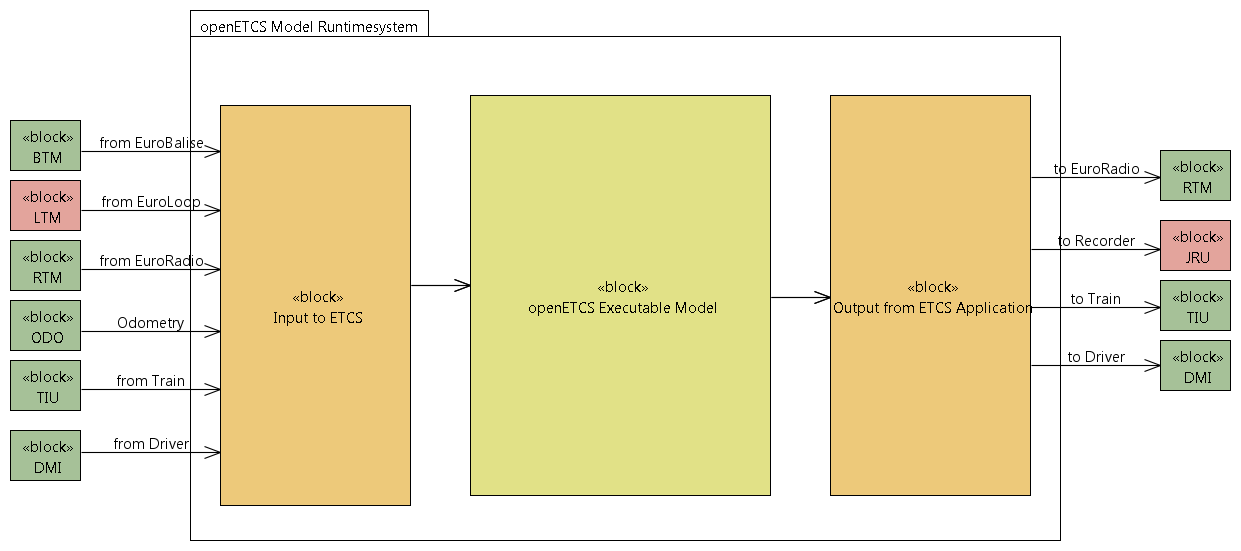
\includegraphics[width=\linewidth]{openETCSAPI.png}
\caption{openETCS API Highlevel View}
\label{fig:apiHighLevel}
\end{figure}

Figure \ref{fig:apiHighLevel} shows the structure of API with respect to the software architecture. Note that red input and output modules are were not yet implemented and thus are not part of the openETCS OBU model. The system covers functions for processing inputs from other units, functions for processing outputs to other functions and a basic runtime system. Inputs are used to feed the input to the executable model before calling it, outputs are used for collecting information provided by the executable model to be passed to the relevant interfaces after the execution cycle has finished.

\section{Principles for Interfaces (openETCS API)}

Information is exchanged via asynchronous \emph{messages}. A message is a set of information corresponding to an event of a particular unit, e.g.~a balise message received from the {BTM}. For possible types of messages please refer to Chapter~\ref{information-flows}.

The information is passed to the executable model as parameters to the synchronous call of a procedure (Interface to the executable model). Since the availability of input messages to the application is not guaranteed the parts of the interfaces are defined with a "present" flag. In addition, fields of input arrays quite often is of variable size. Implementation in the concrete interface in this use-case is the use of a "size" parameter and a "valid"-flag.


\section{openETCS Model Runtime System}
The openETCS model runtime system also provides:
\begin{description}

\item[Input Functions From other Units]
In this entity messages from other connected units are received.

\item[Output Functions to other Units]
The entity writes messages to other connected units.

\item[Conversation Functions for Messages (Bitwalker)]
The conversion function are triggered by Input and Ouput Functions. The main task is to convert input messages from an bit-packed format into logical ETCS messages (the ETCS language) and Output messages from Logical into a bit-packed format. The logical format of the messages is defined for all used types in the openETCS data dictonary.

Variable size elements in the Messages are converted to fixed length arrays with an used elements indicator. Optional elements are indicated with an valid flag.

The conversion routines are responsible for checking the data received is valid. If  faults are detected the information is passed to the openETCS executable model for further reaction. 

\item[Model Cycle]
The version management function is part of the message handling. This implies, conversions from other physical or logical layouts of messages are mapped onto a generic format used in the EVC. Information about the origin version of the message is part of the messages.
 
The executable model is called in cycles. In the cycle 
\begin{itemize}
\item First the received input messages are decoded
\item The input data is passed to the executable model in a predefined order. \textbf{(Details for the interface to be defined)}.
\item Output is encoded according to the {SRS} and passed to the  buffers to the units.
\end{itemize}
\end{description}


\section{Input Interfaces of the openETCS API From other Units of the OBU}
Interfaces are defined in the Scade project APITypes (package API\_Msg\_Pkg.xscade).

In the interfaces the following principles for indicating the quality of the information is used:


\tablefirsthead{
\hline 
\rowcolor{gray} 
Indicator & Type & Purpose \\\hline}
\begin{supertabular}{| p{2 cm} | p{2 cm} | p{8 cm} |}
present & bool & True indicates the component has been changed compared to the previous call of the routine
\\\hline 
valid & bool & True indicates the component is valid to be used. 
\\\hline 
\end{supertabular}

In the next table we can see the interfaces being used in the openETCS system. Details on the interfaces are defined further down.

\tablefirsthead{
\hline 
\rowcolor{gray} 
Unit & Name &  Processing Function  \\\hline}
%\begin{itemize}{| m{1.2cm} | m{1.5cm} | m{1.2cm} | m{3.7cm}  | m{3.7cm} |}
\begin{supertabular}{| c | c | c |}
{BTM} & Balise Telegram & Receive Messages  \\\hline
{DMI} & Driver Machine Interface & DMI Manager  \\\hline
EURORADIO & Communication Management & Communication Management  \\\hline
EURORADIO & Radio Messages & Receive Messages  \\\hline
{ODO} & Odometer & All Parts \\\hline
System TIME & Time system of the OBU & All Parts \\\hline
TIU & Train Data & All Parts \\\hline
\end{supertabular}

Information in the following sections gives an more detailed overview of the structure of the interfaces.


\section{Message based interface (BTM, RTM)}


Balise Message (Track to Train)

\tablefirsthead{
\hline 
\rowcolor{gray} 
Message Name & Optional Packets & Restrictions in the current scope \\\hline}
\begin{supertabular}{| p{4 cm} | p{6 cm} | p{4,5 cm} |}
Balise Telegram &
3: National Values \newline
41: Level Transition Order \newline
42: Session Management  \newline
45: Radio Network registration \newline
46: Conditional Level Transition Order \newline
65: Temporary Speed Restriction \newline
66: Revoke Temporary Speed Restriction \newline
72: Packet for sending plain text messages \newline
137: Stop if in Staff Responsible \newline
255: End of Information \newline
& Used in Scenario
\\\hline
Balise Telegram &
0, 2, 3, 5, 6, 12, 16, 21, 27, 39,
40, 41, 42, 44, 45, 46, 49, 51, 52, 65,
66, 67, 68, 69, 70, 71, 72, 76, 79, 80,
88, 90, 131, 132, 133, 134, 135, 136, 137, 138,
139, 141, 145, 180, 181, 254
&  Not Used in Scenario\\\hline
\end{supertabular}

Radio Messages (Track to Train)

\tablefirsthead{
\hline 
\rowcolor{gray} 
Message Name & Optional Packets & Restrictions in the current scope \\\hline}
\begin{supertabular}{| p{4 cm} | p{6 cm} | p{4,5 cm} |}
2: SR Authorisation & 63:\ List\ of\ Balises\ in\ SR Authority & Message Not Supported \\\hline
3: Movement Authority &
 21:\ Gradient\ Profile\newline
 27: International Static Speed Profile\newline
 49: List of balises for SH Area\newline
 80: Mode profile\newline
 plus common optional packets\newline
 & a \\\hline
9: Request To Shorten MA &
 49: List of balises for SH Area\newline
 80: Mode profile\newline 
& \\\hline
24: General Message &
From RBC:\newline
 21:\ Gradient\ Profile\newline
 27: International Static Speed Profile\newline
 plus common optional packets\newline
From RIU:\newline 44, 45, 143, 180, 254
& Messages from RIU are not supported \\\hline
28: SH authorised & 3, 44, 49
& \\\hline
33: MA with Shifted Location Reference &
 21:\ Gradient\ Profile\newline
 27: International Static Speed Profile\newline
 49: List of balises for SH Area\newline
 80: Mode profile\newline
 plus common optional packets\newline
& \\\hline
37: Infill MA &
5, 21, 27, 39, 40, 41, 44, 49, 51, 52, 65, 66, 68, 69, 70, 71, 80, 88, 138, 139 
 & Message Not Supported \\\hline
List of common optional parameters &
3, 5, 39, 40, 51, 41, 42, 44, 45, 52, 57, 58, 64, 65, 66, 68, 69, 70, 71, 72, 76, 79, 88, 131, 138, 139, 140, 180
& \\\hline
\end{supertabular}

The runtime system is in charge to transfer the messages from its stream mode first to  compressed message format. 

\section{Interfaces to the Time System}
The interface types are defined in the OBU\_Basic\_Types\_Pkg Package. The system time is defined in the basic software.

The system TIME is provided to the executable model at the begin of the cycle. It is not refreshed during the cycle. The time provided to the application is equal to 0 at power-up of the EVC (it is not a “UTC time” nor a “Local
Time”), then must increase at each cycle (unit = 1 msec), until it reaches its maximum value (i.e current EVC
limitation = 24 hours)

\begin{itemize}
\item TIME (T\_internal\_Type, 32-bit INT)\\
Standardized system time type used for all internal time calculations: in ms. The time is defined as a cyclic counter: When the maximum is exceeded the time starts from 0 again. 

\item CLOCK (to be implemented)\\
The clocking system is provided by the JRU. A GPS based clock is assumed to provide the local time.

\end{itemize}

\section{Interfaces to the Odometry System}
The interface types are defined in the OBU\_Basic\_Types\_Pkg Package. 
The odometer gives the current information of the positing system of the train. In this section the structure of the interfaces are only highlighted. Details, including the internal definitions for distances, locations speed and time are implemented in the package. 

\begin{itemize}
\item Odometer (odometry\_T)
\begin{itemize}
\item valid (bool)\\
valid flag, i.e., the information is provided by the ODO system and can be used.
\item timestamp (T\_internal\_Type)\\
of the system when the odometer information was collected. Please, see also general remarks on the time system. 
\item Coordinate (odometryLocation\_T)
\begin{itemize}
\item nominal (L\_internal\_Type) [cm]
\item min (L\_internal\_Type) [cm]
\item max (L\_internal\_Type) [cm]
\end{itemize}
The type used for length values is a 32 bit integer. 
Min and max value give the interval where the train is to be expected. The bounderies are determined by the inaccuracy of the positioning system. All values are set to 0 when the train starts.

\item speed (OdometrySpeeds\_T) [km/h]
\begin{itemize}
\item v\_safeNominal (speed internal type) [km/h]\\
The safe nominal estimation of the speed which will
be bounded between 98\% and 100\% of the upper
estimation
\item v\_rawNominal (speed internal type) [km/h]\\
The raw nominal estimation of the speed which will
be bounded between the lower and the upper
estimations
\item v\_lower (speed internal type) [km/h]\\
The lower estimation of the speed
\item v\_upper (speed internal type) [km/h]\\
The upper estimation of the speed
\end{itemize}
The type used for speed values is a 32 bit integer. 
Min and max value give the interval where the train is to be expected. The bounderies are determined by the inaccuracy of the positioning system. All values are set to 0 when the train starts.
\item acceleration (A\_internal\_Type)[0.01 m/s2],\\
Standardized acceleration type for all internal calculations : in 
\item motionState (Enumeration)\\
indicates whether the train is in motion or in no motion
\item motionDirection (Enumeration)\\
indicates the direction of the train, i.e., CAB-A first, CAB-B first or unknown.
\end{itemize}
\end{itemize}

\section{Interfaces to the Train Interfaces (TIU)}
The following infomration is based on the implementation of the Alstom API. The interface is organised in packets. The packets of the Alstom implementation are listed in the appendix to this document.

The description of interfaces needed for the current scope will be added according to the use.

\section{Output Interfaces of the openETCS API TO other Units of the OBU}

\tablefirsthead{
\hline 
\rowcolor{gray} 
From Function & Name &  To Unit & Description \\\hline}
%\begin{supertabular}{| m{1.2cm} | m{1.5cm} | m{1.2cm} | m{3.7cm}  | m{3.7cm} |}
\begin{supertabular}{| c | c | c | c  | c |}
 & Radio Output Message & \ EURORADIO & \\\hline
 & Communication Management  &  EURORADIO  & \\\hline
 & Driver Information & {DMI} & \\\hline
 & Train Data  & TIU &  
\\\hline
\end{supertabular}

Packets:
to be completed

Radio Messages
to be completed


%-----------------------------------------------------------------------
%\subsection{Runtime- APIl}
%-----------------------------------------------------------------------
%\tbc
%JakobGärtner


\chapter{System Architecture}\todo[fancyline]{has to be completed}
%set the master document for easy compilation
%!TEX root = ../D3_5_3.tex

The figure below shows the system scope for design of the ETCS Subsystem regarding the openETCS Onboard Unit and the Test Environment within the scope of the openETCS project proof of conept on ETCS Level 2 Utrecht - Amsterdam.

\section{System Structure from the subchapter 2.4. of ERA TSI Subset 26 chapter 2}
See Figure~\ref{Scope of System according to ERA TSI Chapter 2}.
\begin{figure}
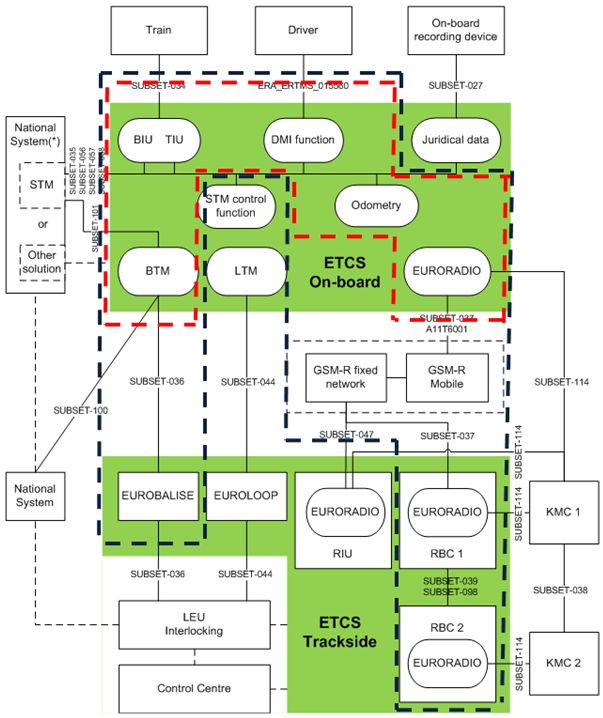
\includegraphics[width=.9\textwidth]{images/ArchitectureSRS}
\caption{Scope of system according to ERA TSI Chapter 2.}
\label{Scope of System according to ERA TSI Chapter 2}
\end{figure}

\section{System Architecture SysML View}
The SysML System view of the architecture will reflect the scope accorgin to 4.1 and is a top down breakdown to the design layer. The functional breakdown has been done in Scade System and is part of the design model. Furthermore it will reflect all the external and internal interface that will will be described in 4.3. Another goal of the System Architecture SysML view is to explain and set the boundaries for the ETCS Kernel development "F2 Kernel" as the main design part of the openETCS@ITEA2 project.

\subsection{1st Level System Architecture View}
All subystem of the ETCS/ERTMS Basic Sytem according in the scope of the openETCS@ITEA2 project will be reflected in this 1st level view. Furthermore the interlocking as part of a full Rail Signalling System, but not part of the openETCS scope, will be highlighted in this view.

Interlocking =  interlocking is an arrangement of signal apparatus that prevents conflicting movements through an arrangement of tracks such as junctions or crossings. The signalling appliances and tracks are sometimes collectively referred to as an interlocking plant. An interlocking is designed so that it is impossible to display a signal to proceed unless the route to be used is proven safe.


\begin{figure}
\centering
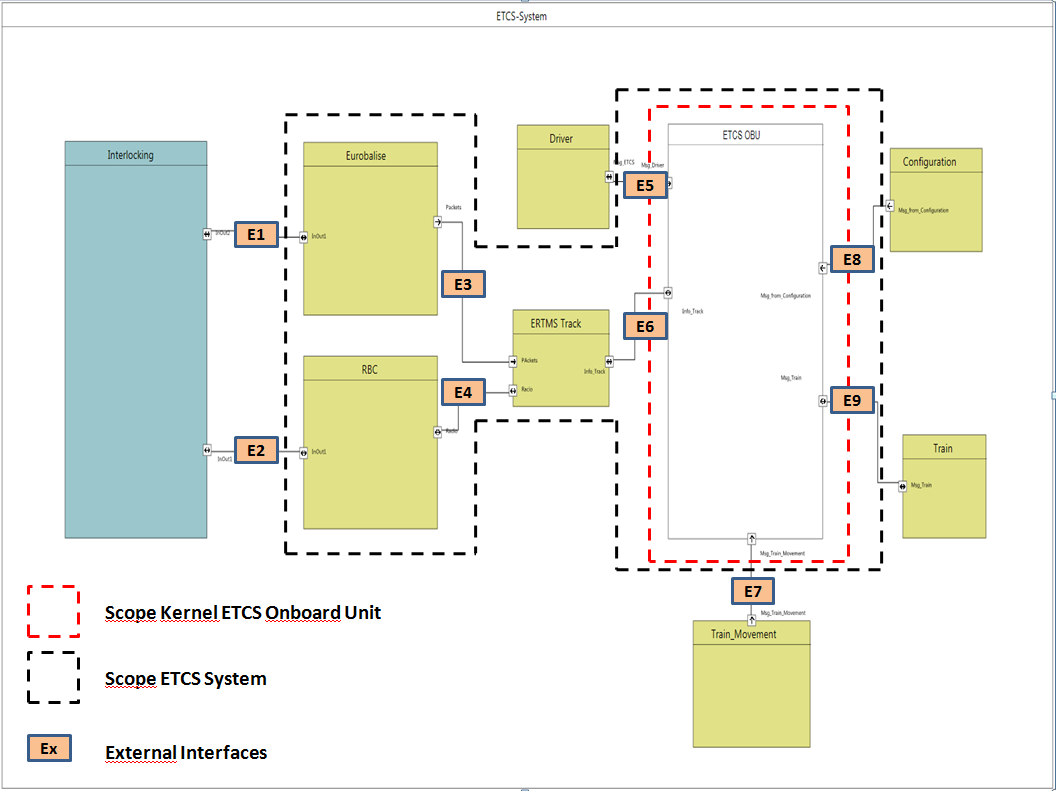
\includegraphics[scale=0.6]{images/1stlevelarchitecture}
\caption{1st level system architecture view.}
\label{1st level System Architecture view}
\end{figure}

\subsection{2nd Level System Architecture View}
The 2nd level system view will provide a decopmosition of the ETCS on-board unit systems and the Kernerl of the ETCS. The kernel is the main part of the ETCS Onboard Unit system and reflects the functions specified in the ERA TSI Subset 26. Therefore, the boundaries and interfaces to the other subasystems of the ETCS on-bard unit needs to be fully described and formal. At least the formalisation kernel functions and boundaries should be realized in the openETCS project.

\begin{figure}
\centering
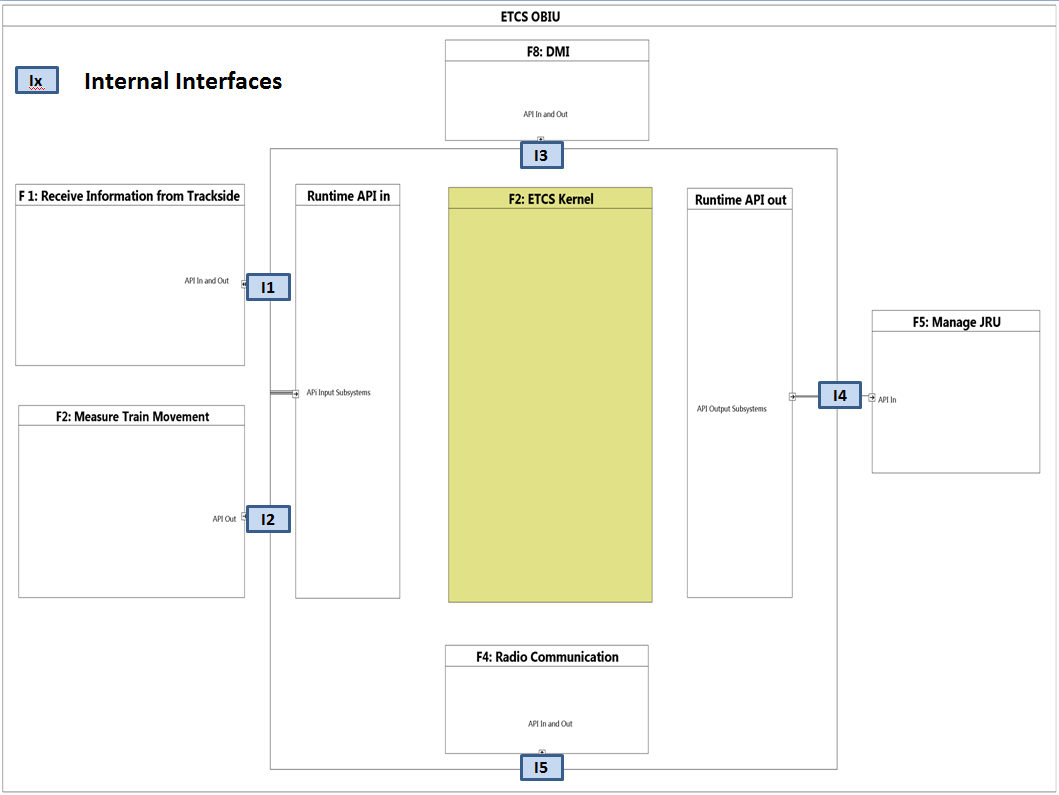
\includegraphics[scale=0.6]{images/2ndlevelarchitecture}
\caption{2nd level system architecture view.}
\label{2nd level System Architecture view}
\end{figure}

\subsection{3rd Level System Architecture View}
The 3rd level system view will provide a decopmosition of the ETCS Kernel of the ETCS Onboard Unit Systems. The decomposition and further design of the subfunctions of the kernel are part of the chapter 6 in this document. In chapter 6 we will consider the design description that will be completed by every designer itself. The designer can decided in this layer about the decomposition and boundaries of his subsystem, but need to describe the design choices.


\section{Interfaces}
This section will consider the external and internal interfaces as described in the system decomposition figures in 4.2.1 and 4.2.2.

\subsection{External Interfaces}
External interfaces will describe the data flow between the Systems outside of the scope of the openETCS Project and the ETCS Onboard Unit System.

\begin{description}
\item[E1:] In- and out flow between the Interlocking an Eurobalise. There will be 2 kind of balises
\begin{itemize}
\item Fixed Balise: no interaction to the interlocking
\item Balise Controlled: interaction to the interlocking trough LEU
\end{itemize}
\begin{figure}
\centering
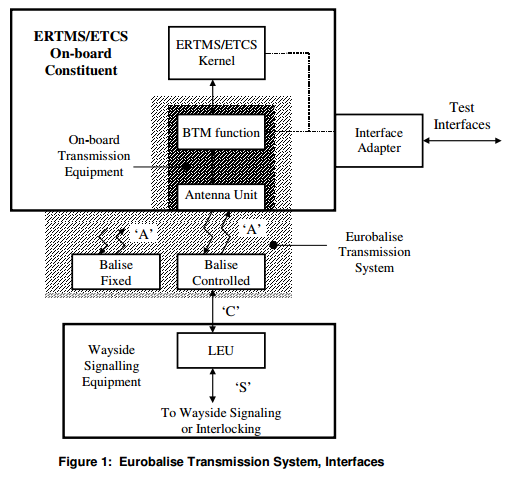
\includegraphics[scale=0.8]{images/Eurobalise}
\caption{Eurobalise}
\label{Eurobalise}
\end{figure}

\item[E2:] In- and out flow between the Interlocking and Radio Block Control.
This External interface will ensure the states or logics directly to the Radio Block Control and the other way back from the train to the interlocking.

\item[E3:] Input flow from the Eurobalise to the Balise Transmission Module or Antenna Unit (BTM) into the ETCS Onboard Unit. As already described on the figure in E1.

\item[E4:] In- and out flow between the Radio Block Control and the Euroradio Modul into the ETCS Onboard Unit. This interface is not in Level 0 or 1 active since there is no necessary for ETCS Radio interaction between track and train.

\item[E5:] This interface will describe the interaction between the Human and Display (Human Machine Interface or Driver Machine Interface), c.f.~Figure \ref{DMI Interfaces}.
\begin{figure}
\centering
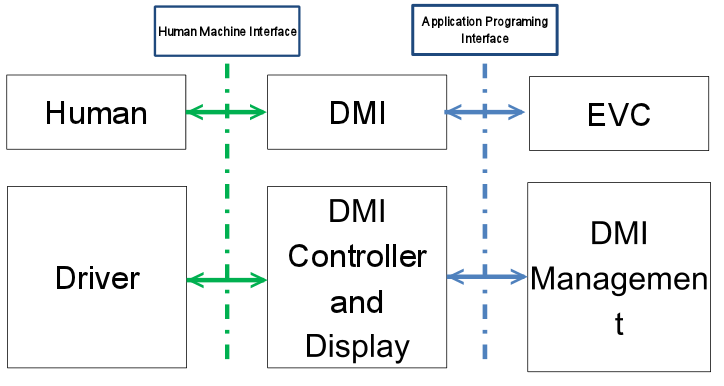
\includegraphics[scale=0.6]{images/DMIinterfaces}
\caption{DMI Interfaces.}
\label{DMI Interfaces}
\end{figure}

\item[E6:] This interface is composite the interfaces E3 and E4.

\item[E7:] Input interface to the odometry Subsystem of the ETCS Onboard System. Will send information to train if there is any movement outside the ETCS System is leading such as "cold movement".

\item[E8:] Input interface to the ETCS Onboard Unit system to set configuration data such as fixed values, system values, national values and train configuration.

\item[E9:] In- and Out flow between the ETCS Onboard Unit System and the Train. This interface will describe the itneraction between the Train and the ETCS Onboard Unit System such as brake controll, traction control, door control, ....
\end{description}


\subsection{Internal Interfaces}
Internal interfaces will describe the data flow between the ETCS Onboard Unit Kernel and ETCS Onboard Unit Subsystems within the ETCS Onboard Unit System.

\begin{description}
\item[I1:] In flow from the Balise Transmission Module (BTM or Antenna) to the "F2 ETCS Kernel" trough Runtime API in. Transmitted data are information from the Eurobalise.

\item[I2:] In flow from the Odometrie (ODO) to the "F2 ETCS Kernel" trough Runtime API in. Transmitted data are information from the Movement of the train.

\item[I3:] In- and Out flow between the DMI Controller and the "F2 ETCS Kernel" trough Runtime API in and out. Transmitted data are information of driver action and display. See description in figure of "External Interface E5".

\item[I4:] Out flow from "F2 ETCS Kernel" to the JRU Manager trough Runtime API out. Transmitted data are all necessary information for a juridical recorder unit "black box".

\item[I5:] In- and Out flow between the Euroradio and "F2 ETCS Kernel" trough Runtime API in and out. Transmitted data are radio track information (RBC) and information to the track (RBC). 
\end{description}




%\chapter{Software Architecture}
%t.b.d.\todo[fancyline]{has to be completed}



\part{Design Description}

\chapter{General Design Decisions}

\chapter{F1: Receive Information from Trackside}

%set the master document for easy compilation
%!TEX root = ../D3_5_3.tex

\section{ETCS Messaging: TrackMessages}

\todo[inline]{section needs to be completed}
\subsection{Component Requirements}

\begin{longtable}{p{.25\textwidth}p{.7\textwidth}}
\toprule
Component name			& TrackMessages::Read\_P005 \\
\midrule
Link to SCADE model		& {\footnotesize \url{https://github.com/openETCS/modeling/tree/master/model/Scade/System/ObuFunctions/ETCS_Messaging/TrackMessages}} \\
\midrule
SCADE designer			& Jakob G\"artner, LEA Railergy \newline
Mairamou Haman Adji, LEA Railergy\\
\midrule
Description				& TrackMessages is a library containing functionality to:
\begin{itemize}
\item Transport TrainToTrack and TrackToTrain messages and packets using a compressed format which is conceptually close to the ETCS language as defined in Subset-026
\item Compress trackside information and decompress it in the onboard unit, taking into account different baseline versions and providing transparent translation.
\item Compress trainside information and decompress it in the trackside simulation models, taking into account different baseline versions and providing transparent translation.
\end{itemize}
As TrackMessages is a library with various components supporting all packets and messages defined in Subset-026, we have selected one exemplary function to document the concept. As only the packet/ message- related functionality is specific, this approach will allow a first understanding of the concept and the related interfaces. For a full discussion of the library, refer to the [specifc chapter? document?]\newline
The function Read\_P005 extracts a packet 5 (Gradient Profile) from the compressed packets data flow, if present. It translates the integer- coded compressed data with the help of the metadata in the header section of the CompressedPackets\_T formatted data flow. After performing variable-level translation and exception detection, a baseline-3 conformal packet 5 is available for use within the relevant OBU functions.
\\

\midrule
Input documents	& 
Subset-026, Chapter 6\newline
Subset-026, Chapter 7\newline
Subset-026, Chapter 8\newline
\newline
The objective of this component (the full TrackMessages library) is to provide a full formalisation of above chapters in Subset-026\\
\midrule
Safety integrity level		& 4 \\
\midrule
Time constraints		& n/a (for the provided example function) \\
\midrule
API requirements 		& In the demonstrator context, the API is fully defined on SCADE model level. For integration with external systems (BTM, Radio, Subset-076 or Subset-94), additional conversion to/ from bit-level representation will be required\\
\bottomrule
\end{longtable}


\subsection{Interface}

An overview of the interface of component [component name] is shown in Figure~\ref{f:trackside_interface}. The inputs and outputs are described in detail in Section~\ref{s:trackside_inputs} respectively \ref{s:trackside_outputs}.

\begin{figure}
\center
\missingfigure{[Put SysML diagram of component here]}
\caption{TrackMessages SysML diagram}\label{f:trackside_interface}
\end{figure}


\subsubsection{Inputs}\label{s:trackside_inputs}

\paragraph{Message\_In}

\begin{longtable}{p{.25\textwidth}p{.7\textwidth}}
\toprule
Input name				&Message\_In \\
\midrule
Description				& Message\_In takes the compressed track-to-train messages that have either been compressed by the trackside simulation components of the TrackMessages library, or have been filled by the API. All packets that are part of the same message are transmitted within one cycle of the model's execution. Message\_IN is taking the compressed packet information from the track to train dataflow. \newline
  \\
\midrule
Source					& Manage\_TrackSideInformation\_Integration \\ 
\midrule
Type					& Common\_Types\_Pkg::CompressedPackets\_T \\
\midrule
Valid range of values 	& The consistency of the metadata is checked at the input side. The ranges of the transported variables are checked at the conversion step (from integer format to SRS-conform format)
 \\
\midrule
Behaviour when value is at boundary	& n/a \\
\midrule
Behaviour for values out of valid range	& The content of this input is not checked, as any issues will be found at conversion level. If the metadata are not matching the search criteria the packet will be considered as non existent and will therefore be ignored. 
 \\
\bottomrule
\end{longtable}




\subsubsection{Outputs}\label{s:trackside_outputs}

\paragraph{received}

\begin{longtable}{p{.25\textwidth}p{.7\textwidth}}
\toprule
Output name				& received \\
\midrule
Description				& Flag to indicate reception of a packet 5 from trackside in the current cycle. \\
\midrule
Destination				& Any calling component.
\todo[inline]{components should be listed here}\\ 
\midrule
Type					& bool \\
\midrule
Valid range of values	&
\todo[inline]{to be checked}
\begin{description}
\item[true] Packet 5 has been received  in the current cycle.
\item[false] Packet 5 has not been received in the current cycle.
\end{description}
 \\
\midrule
Behaviour when value is at boundary	& n/a \\
\midrule
Behaviour for values out of valid range	& n/a \\
\midrule
Behaviour when value is erroneous, absent or unwanted (i.e. spurious) & n/a\\
\bottomrule
\end{longtable}


\paragraph{P005\_OBU\_out}

\begin{longtable}{p{.25\textwidth}p{.7\textwidth}}
\toprule
Output name				& P005\_OBU\_out \\
\midrule
Description				& Gradient Profile (Packet 5) according to 7.4.2.2 \\
\midrule
Destination				& Any calling operator\\ 
\midrule
Type					& TM::P005\_OBU\_T\\
\midrule
Valid range of values	& TM::P005\_OBU\_T is a complex data type. Values are given for each element. Format is: Type Name: range/list of values
\begin{itemize}
\item bool valid: [true | false]
\item q\_dir Q\_DIR:\newline  [Q\_DIR\_Both\_directions |\newline Q\_DIR\_Nominal |\newline Q\_DIR\_Reverse]
\item l\_packet L\_PACKET: (0-8191)
\item q\_scale Q\_SCALE: \newline[ENUM\_Q\_SCALE\_10cm |\newline ENUM\_Q\_SCALE\_1m |\newline ENUM\_Q\_SCALE\_10m]
\item n\_iter N\_ITER: (0-33) \emph{(Remark: start section from the original packet is integrated into the list of sections)}
\end{itemize}
The structured element sections is an array of type P005\_section\_enum\_T. For each element, the valid range of values is as follows:
\begin{itemize}
\item bool valid: [true | false] \emph{(Remark: Check for consistency with the value of n\_iter)}
\item d\_link D\_LINK: (0-32767)
\item q\_newcountry Q\_NEWCOUNTRY:\newline [TM\_conversions::ENUM\_Q\_NEWCOUNTRY\_same |\newline TM\_conversions::ENUM\_Q\_NEWCOUNTRY\_not\_same]
\item nid\_c NID\_C: (0-1023)
\item nid\_bg NID\_BG: (0-16383)
\item q\_linkorientation Q\_LINKORIENTATION:\newline [TM\_conversions::ENUM\_Q\_LINKORIENTATION\_reverse|\newline TM\_conversions::ENUM\_Q\_LINKORIENTATION\_nominal]
\item q\_linkreaction Q\_LINKREACTION:\newline [TM\_conversions::ENUM\_Q\_LINKREACTION\_Train\_trip |\newline TM\_conversions::ENUM\_Q\_LINKREACTION\_Apply\_service\_brake\newline TM\_conversions::ENUM\_Q\_LINKREACTION\_No\_Reaction]
\item q\_locacc Q\_LOCACC: (0-63)
\end{itemize}

\emph{Only an output structure with the structured element "valid" set to "true" is to be considered as received. If this field is set to true, the Output 1 (received) must equally be set to "true".}

 

 \\
\midrule
Behaviour when value is at boundary	& n/a \\
\midrule
Behaviour for values out of valid range	& The component is prepared for the upcoming error/exception handling concept. An error flag is, at the moment, raised internally if any of the compressed input values is out of range. A hierarchical error processing is foreseen.\newline
The types that have been defined in the package S026\_7 do not provide any default/ invalid value. The following fields are therefore set to an arbitrary value upon reception of an out-of-range value from track side, and the internal error flag is raised:
\begin{itemize}
\item q\_dir Q\_DIR:\newline  set to: Q\_DIR\_Both\_directions
\item q\_scale Q\_SCALE: \newline set to: ENUM\_Q\_SCALE\_10cm 
\item q\_newcountry Q\_NEWCOUNTRY:\newline set to:[TM\_conversions::ENUM\_Q\_NEWCOUNTRY\_same |\newline TM\_conversions::ENUM\_Q\_NEWCOUNTRY\_not\_same]
\item q\_newcountry Q\_NEWCOUNTRY:\newline set to: TM\_conversions::ENUM\_Q\_NEWCOUNTRY\_not\_same
\item q\_linkorientation Q\_LINKORIENTATION:\newline set to: TM\_conversions::ENUM\_Q\_LINKORIENTATION\_reverse
\item q\_linkreaction Q\_LINKREACTION:\newline set to: TM\_conversions::ENUM\_Q\_LINKREACTION\_Train\_trip
\end{itemize}

 \\
\midrule
Behaviour when value is erroneous, absent or unwanted (i.e. spurious) & n/a \\
\bottomrule
\end{longtable}


\subsection{Subcomponents}

\subsubsection{Read\_Packets}
%set the master document for easy compilation
%!TEX root = ../D3_5_3.tex

%\section{ETCS Messaging: TrackMessages}

\subsection{Component Requirements}

\begin{longtable}{p{.25\textwidth}p{.7\textwidth}}
\toprule
Component name			& TM\_lib\_internal::RECV\_ReadPackets \\
\midrule
Link to SCADE model		& {\footnotesize \url{https://github.com/openETCS/modeling/tree/master/model/Scade/System/ObuFunctions/ETCS_Messaging/TrackMessages}} \\
\midrule
SCADE designer			& Jakob G\"artner, LEA Railergy\\
\midrule
Description				& RECV\_ReadPackets extracts packet data information and raw compressed packet data from the compressed packets data flow, using filter criteria provided through parameter inputs:\newline
\begin{itemize}
\item NID\_PACKET: search for a specific packet
\item Version Number: search for a specific version number
\item Q\_DIR: search for packets that are only valid for a specific direction
\item Serial number: search for a specific packet instance, if several instances of a given packet type exist
\item F\_Version: Flag to decide whether to evaluate or ignore packet version information.
\item F\_id: Flag whether to evaluate or ignore packet serial number information.\newline
\end{itemize}

The operator TM\_lib\_internal::RECV\_ReadPackets takes a set of parameter data to 

\begin{itemize}
\item 1. Search the metadata of the compressed packets data flow using the provided parameters to determine if a matching packet is contained in any given cycle
\item 2. Output the flag "received" exactly in any cycle a matching packet is found
\item 3. Output an array of compressed packet data that is filled with the data from the identified packet
\end{itemize}


\\

\midrule
Input documents	& 
Subset-026, Chapter 7\newline
\newline
This function is not directly traceable to Subset-026, but is built from derived requirements\\
\midrule
Safety integrity level		& 4 \\
\midrule
Time constraints		& n/a  \\
\midrule
API requirements 		& In the demonstrator context, the API is fully defined on SCADE model level. For integration with external systems (BTM, Radio, Subset-076 or Subset-94), additional conversion to/ from bit-level representation will be required\\
\bottomrule
\end{longtable}
%-------------------------------------------------------------------------------------------------------------------------
%-------------------------------------------------------------------------------------------------------------------------
%-------------------------------------------------------------------------------------------------------------------------


\subsection{Interface}

An overview of the interface of component [component name] is shown in Figure~\ref{f:trackside_interface}. The inputs and outputs are described in detail in Section~\ref{s:trackside_inputs} respectively \ref{s:trackside_outputs}.

\begin{figure}
\center
\missingfigure{[Put SysML diagram of component here]}
\caption{Component SysML diagram}\label{f:trackside_interface}
\end{figure}

%-------------------------------------------------------------------------------------------------------------------------
%-------------------------------------------------------------------------------------------------------------------------


\subsubsection{Inputs}\label{s:trackside_inputs}

%-------------------------------------------------------------------------------------------------------------------------


\paragraph{Message\_In}

\begin{longtable}{p{.25\textwidth}p{.7\textwidth}}
\toprule
Input name				&Message\_In \\
\midrule
Description				& Message\_In takes the compressed track-to-train messages that have either been compressed by the trackside simulation components of the TrackMessages library, or have been filled by the API. All packets that are part of the same message are transmitted within one cycle of the model's execution. Message\_IN is taking the compressed packet information from the track to train dataflow. \newline
  \\
\midrule
Source					& Manage\_TrackSideInformation\_Integration through any calling operator (TM::Read\_Pxxx) \\ 
\midrule
Type					& Common\_Types\_Pkg::CompressedPackets\_T \\
\midrule
Valid range of values 	& n/a\newline
The consistency of the metadata is checked at the input side.\newline
The ranges of the transported variables are checked at the conversion step (from integer format to SRS- conformal format)
 \\
\midrule
Behaviour when value is at boundary	& n/a \\
\midrule
Behaviour for values out of valid range	& n/a \newline \newline
The content of this input is not checked, as any issues will be found at conversion level. If the metadata are not matching the search criteria the packet will be considered as non existent and will therefore be ignored. 
 \\
\bottomrule
\end{longtable}

%-------------------------------------------------------------------------------------------------------------------------


\paragraph{PacketID}

\begin{longtable}{p{.25\textwidth}p{.7\textwidth}}
\toprule
Input name				&PacketID \\
\midrule
Description				& PacketID defines the criteria used to determine whether the compressed packets contain a packet of interest. \newline
The information is position coded into an integer:\newline
The format is PPPDVVSSS.
\begin{itemize}
\item PPP: NID\_PACKET according to 7.5.1.93. 3-digit format, leading zeros are omitted.
\item D: Q\_DIR according to 7.5.1.103. 1- digit integer representing the decimal conversion of the binary values defined in 7.5.1.103
\item VV: M\_VERSION according to 7.5.1.79. 2- digit integer representing the decimal conversion of the binary values defined in 7.5.1.79
\item SSS: Serial number: search for a specific packet instance, if several instances of a given packet type exist. For packets where this is relevant, the serial number is used to identify a packet instance according to SRS definition, for example for NID\_TSR.
\end{itemize}

  \\
\midrule
Source					& Calling function  (TM::Read\_Pxxx). This input is realised as a SCADE hidden input, allowing the calling function to provide the information as a parameter \\ 
\midrule
Type					& int \\
\midrule
Valid range of values 	& 
\begin{itemize}
\item PPP: NID\_PACKET 0-999. Values that are not contained in the list of packets 7.4.1.1 are ignored.
\item D: 0-3. Values that are not defined in 7.5.1.103 are ignored
\item VV: 0-99. Values that are not defined in 7.5.1.79 are ignored
\item SSS:0-999
\end{itemize}
.\newline

 \\
\midrule
Behaviour when value is at boundary	& n/a \\
\midrule
Behaviour for values out of valid range	& n/a \newline \newline
As the metadata are automatically encoded using the values for NID\_PACKET, Q\_DIR, M\_VERSION and the serial number when a packet is compressed at trackside, out-of-range values may lead to erroneous identification of packet data. \newline
A static validation of the parameters used by the calling function is required. 
 \\
\bottomrule
\end{longtable}

%-------------------------------------------------------------------------------------------------------------------------


\paragraph{F\_version}

\begin{longtable}{p{.25\textwidth}p{.7\textwidth}}
\toprule
Input name				&F\_version \\
\midrule
Description				& F\_version is a flag. If set to true, version information will be taken into account when looking for a packet.\newline

  \\
\midrule
Source					& Calling function  (TM::Read\_Pxxx). This input is realised as a SCADE hidden input, allowing the calling function to provide the information as a parameter \\ 
\midrule
Type					& bool \\
\midrule
Valid range of values 	& [true | false]
.\newline

 \\
\midrule
Behaviour when value is at boundary	& n/a \\
\midrule
Behaviour for values out of valid range	& n/a  \newline
 \\
\bottomrule
\end{longtable}

%-------------------------------------------------------------------------------------------------------------------------

\paragraph{F\_id}

\begin{longtable}{p{.25\textwidth}p{.7\textwidth}}
\toprule
Input name				&F\_id \\
\midrule
Description				& F\_id is a flag. If set to true, serial number information will be taken into account when looking for a packet.\newline

  \\
\midrule
Source					& Calling function  (TM::Read\_Pxxx). This input is realised as a SCADE hidden input, allowing the calling function to provide the information as a parameter \\ 
\midrule
Type					& bool \\
\midrule
Valid range of values 	& [true | false]
.\newline

 \\
\midrule
Behaviour when value is at boundary	& n/a \\
\midrule
Behaviour for values out of valid range	& n/a  \newline

 \\
\bottomrule
\end{longtable}

%-------------------------------------------------------------------------------------------------------------------------
%-------------------------------------------------------------------------------------------------------------------------

\subsubsection{Outputs}\label{s:trackside_outputs}


\paragraph{Data}

\begin{longtable}{p{.25\textwidth}p{.7\textwidth}}
\toprule
Output name				& Data \\
\midrule
Description				& Contents of the packet, in integer array format. The first n elements of this array contain the data, trailing 0 that are beyond the length of the packet described in the metadata can be ignored. \\
\midrule
Destination				& Any calling operator\\ 
\midrule
Type					& Common\_Types\_Pkg::CompressedPacketData\_T\\
\midrule
Valid range of values	& n/a 

 \\
\midrule
Behaviour when value is at boundary	& n/a \\
\midrule
Behaviour for values out of valid range	& n/a\newline


 \\
\midrule
Behaviour when value is erroneous, absent or unwanted (i.e. spurious) & n/a \\
\bottomrule
\end{longtable}

%-------------------------------------------------------------------------------------------------------------------------


\paragraph{Metadata}

\begin{longtable}{p{.25\textwidth}p{.7\textwidth}}
\toprule
Output name				& Metadata \\
\midrule
Description				& Raw Metadata for the found packet \\
\midrule
Destination				& Any calling operator\\ 
\midrule
Type					& Common\_Types\_Pkg::MetadataElement\_T\\
\midrule
Valid range of values	& n/a 

 \\
\midrule
Behaviour when value is at boundary	& n/a \\
\midrule
Behaviour for values out of valid range	& n/a\newline


 \\
\midrule
Behaviour when value is erroneous, absent or unwanted (i.e. spurious) & n/a \\
\bottomrule
\end{longtable}

%-------------------------------------------------------------------------------------------------------------------------

\paragraph{received}

\begin{longtable}{p{.25\textwidth}p{.7\textwidth}}
\toprule
Output name				& received \\
\midrule
Description				& Flag to indicate reception of a packet 5 from trackside in the current cycle \\
\midrule
Destination				& Any calling component\\ 
\midrule
Type					& bool \\
\midrule
Valid range of values	&
[true | false]
 \\
\midrule
Behaviour when value is at boundary	& n/a \\
\midrule
Behaviour for values out of valid range	& n/a \\
\midrule
Behaviour when value is erroneous, absent or unwanted (i.e. spurious) & n/a\\
\bottomrule
\end{longtable}



%\subsection{Sub Components}

%\subsubsection{Name\_of\_Subcomponent}
%\input{sections/Name\_of\_Subcomponent.tex}

\subsubsection{Extract Packet 5}
%set the master document for easy compilation
%!TEX root = ../D3_5_3.tex

%\section{ETCS Messaging: TrackMessages}

\subsubsection{Component Requirements}

\begin{longtable}{p{.25\textwidth}p{.7\textwidth}}
\toprule
Component name			& TM\_conversions::trackside.C\_P005\_compr\_onboard \\
\midrule
Link to SCADE model		& {\footnotesize \url{https://github.com/openETCS/modeling/tree/master/model/Scade/System/ObuFunctions/ETCS_Messaging/TrackMessages}} \\
\midrule
SCADE designer			& Jakob G\"artner, LEA Railergy\\
\midrule
Description				& If a matching packet 5 has been received, TM\_conversions::trackside.C\_P005\_compr\_onboard: takes the compressed packet data and converts them to an SRS conformal onboard packet format. Trailing 0 beyond the valid length of the packet are ignored. \newline

\\

\midrule
Input documents	& 
Subset-026, Chapter 7\newline
\\
\midrule
Safety integrity level		& 4 \\
\midrule
Time constraints		& n/a  \\
\midrule
API requirements 		& n/a\\
\bottomrule
\end{longtable}
%-------------------------------------------------------------------------------------------------------------------------
%-------------------------------------------------------------------------------------------------------------------------
%-------------------------------------------------------------------------------------------------------------------------




%\subsubsection{Name\_of\_Subcomponent}
%\input{sections/Name\_of\_Subcomponent.tex}


\chapter{F2: ETCS Kernel}

In this chapter we describe the main components of the openETCS OBU model. Section~\ref{s:ETCS_Kernel_Overview} gives an overview of the external interfaces of this functional block and briefly describes the subcomponents. A detailed description of the subcomponents is given in Sections~\ref{s:F2.1} to \ref{s:F2.13}.

\section{ETCS Kernel Overview}\label{s:ETCS_Kernel_Overview}

The ETCS Kernel module consists of the 13 functional components, i.e. F1.1 to F1.13 as depicted in Figures~\ref{f:f2.1_overview} to \ref{f:f2.13_overview}. Note that due to the complexity of the Kernel module the SysML diagram has been splitted into 13 figures. Each of the figures shows one of the subcomponents F2.1 to F2.13 and its connections to the other components in F2 and the inputs respectively outputs of F2. In the following we briefly describe the functionality of these components.
\begin{description}
\item[F2.1: Manage\_TrackSideInformation\_Integration] This component is responsible for receiving Eurobalise telegrams and Euroradio messages from the API and performs several consistency checks on the inputs. The corresponding SysML diagram is shown in Figure~\ref{f:f2.1_overview}. For further details we refer to Section~\ref{s:F2.1}.
\begin{figure}
\center
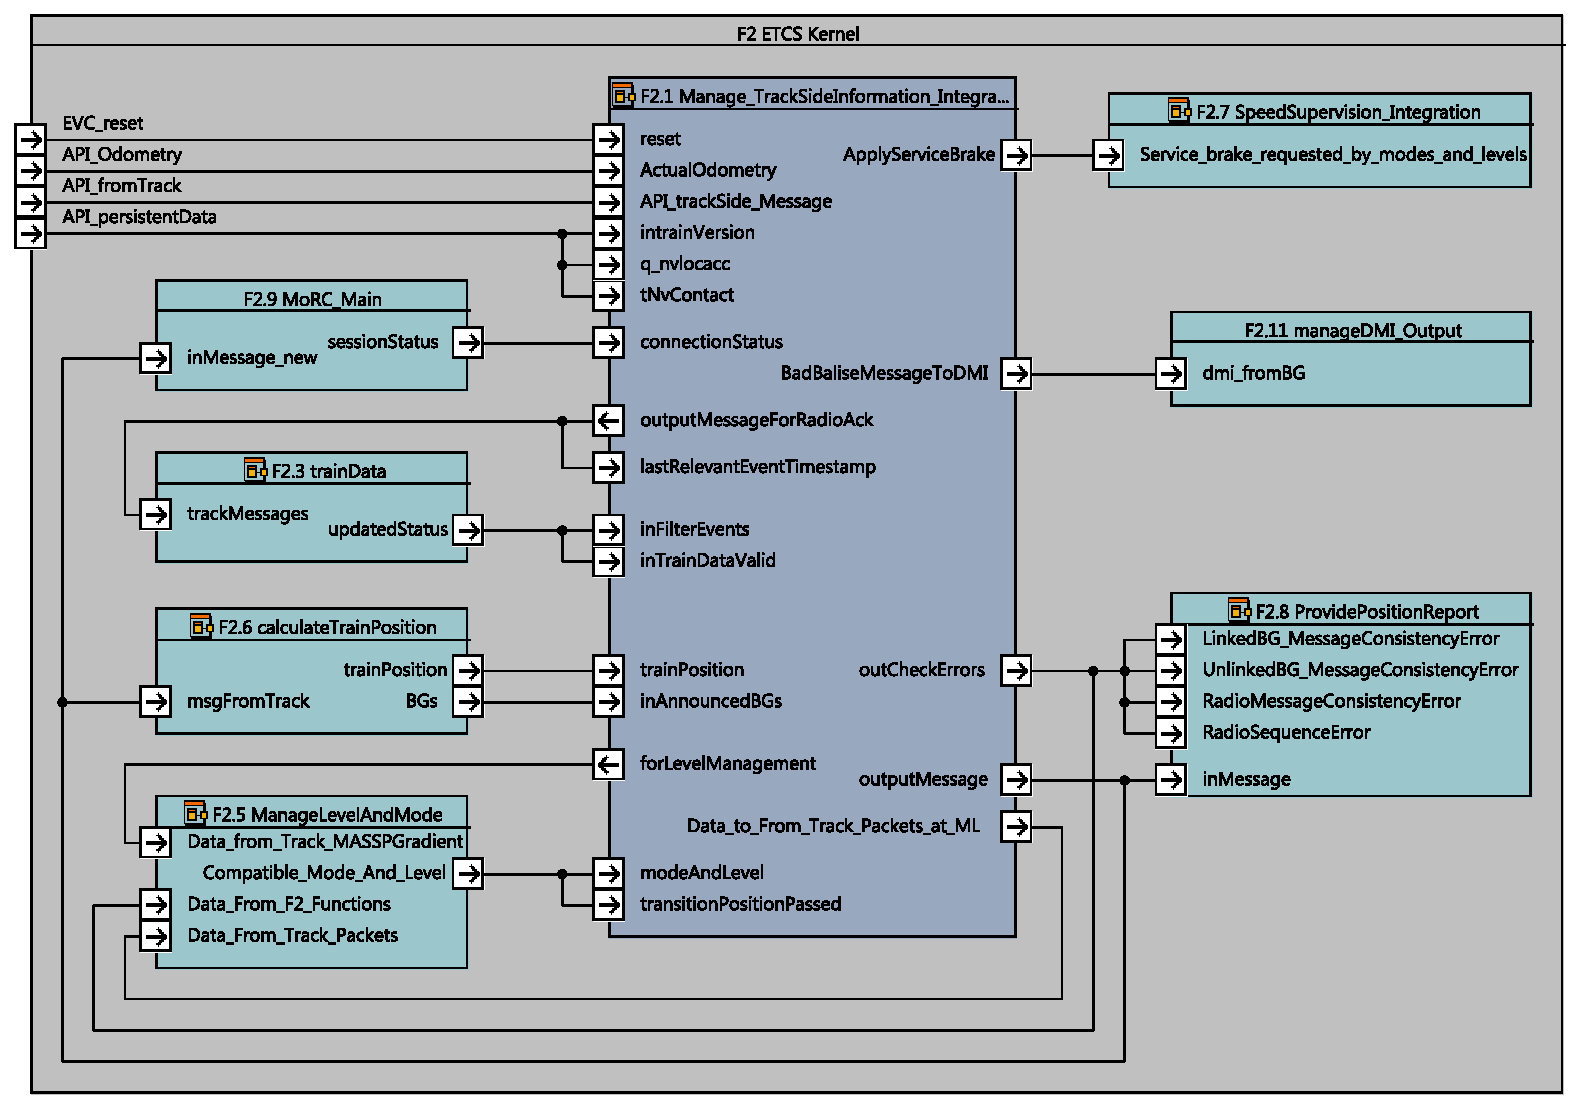
\includegraphics[width=\textwidth]{F2_F2_1.pdf}
\caption{F2: ETCS Kernel SysML diagram with focus on F2.1 Manage\_TrackSideInformation\_Integration component.}\label{f:f2.1_overview}
\end{figure}

\item[F2.2: Manage\_ETCS\_Procedures] This component describes the Start of Mission procedure of the train until the current status will change to another mode, level or other procedure. The corresponding SysML diagram is shown in Figure~\ref{f:f2.2_overview}. For further details we refer to Section~\ref{s:F2.2}.
\begin{figure}
\center
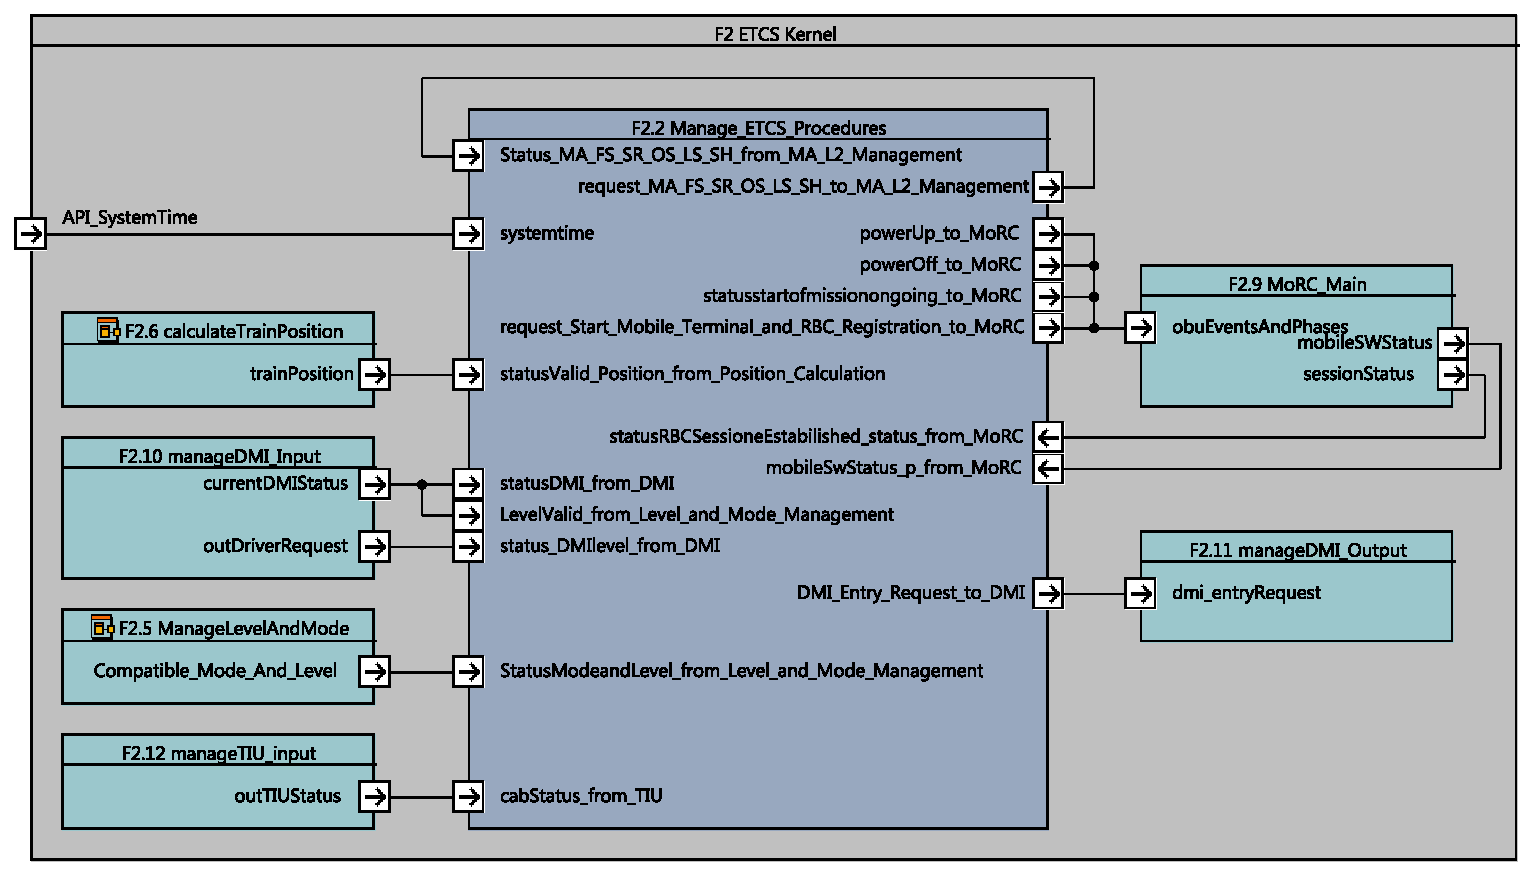
\includegraphics[width=\textwidth]{F2_F2_2.pdf}
\caption{F2: ETCS Kernel SysML diagram with focus on F2.2 Manage\_ETCS\_Procedures component.}\label{f:f2.2_overview}
\end{figure}

\item[F2.3: trainData] Implementation of the train data with the corresponding interfaces to track, driver and RBC. The corresponding SysML diagram is shown in Figure~\ref{f:f2.3_overview}. For further details we refer to Section~\ref{s:F2.3}.
\todo[inline]{descriptions needs to be improved}
\begin{figure}
\center
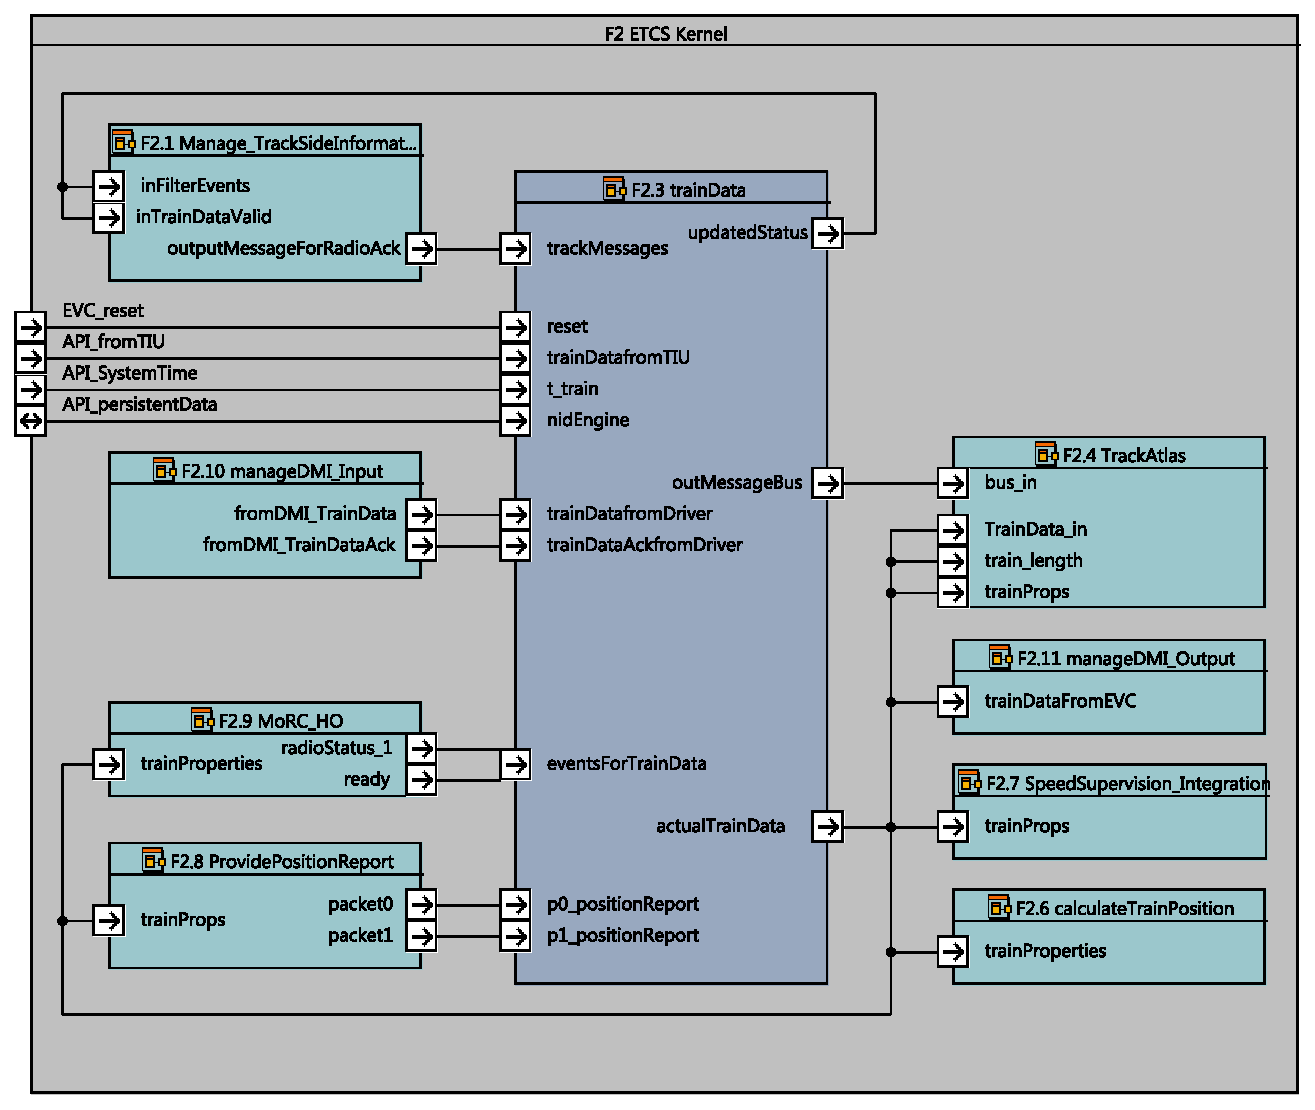
\includegraphics[width=\textwidth]{F2_F2_3.pdf}
\caption{F2: ETCS Kernel SysML diagram with focus on F2.3 trainData component.}\label{f:f2.3_overview}
\end{figure}

\item[F2.4: TrackAtlas] t.b.d.  The corresponding SysML diagram is shown in Figure~\ref{f:f2.4_overview}. For further details we refer to Section~\ref{s:F2.4}.
\todo[inline]{to be completed}
\begin{figure}
\center
\missingfigure{[Put SysML diagram of component here]}
\caption{F2: ETCS Kernel SysML diagram with focus on F2.4 TrackAtlas component.}\label{f:f2.4_overview}
\end{figure}

\item[F2.5: Mode\_and\_Level] Defines the status of the ETCS regarding on-board functional status and track infrastructure. The corresponding SysML diagram is shown in Figure~\ref{f:f2.5_overview}. For further details we refer to Section~\ref{s:F2.5}.
\todo[inline]{descriptions needs to be improved}
\begin{figure}
\center
\missingfigure{[Put SysML diagram of component here]}
\caption{F2: ETCS Kernel SysML diagram with focus on F2.5 Mode\_and\_Level component.}\label{f:f2.5_overview}
\end{figure}

\item[F2.6: calculateTrainPosition] The purpose of this component is to calculate the locations of linked and unlinked balise groups and the current train position while the train is running along the track. The corresponding SysML diagram is shown in Figure~\ref{f:f2.6_overview}. For further details we refer to Section~\ref{s:F2.6}.
\begin{figure}
\center
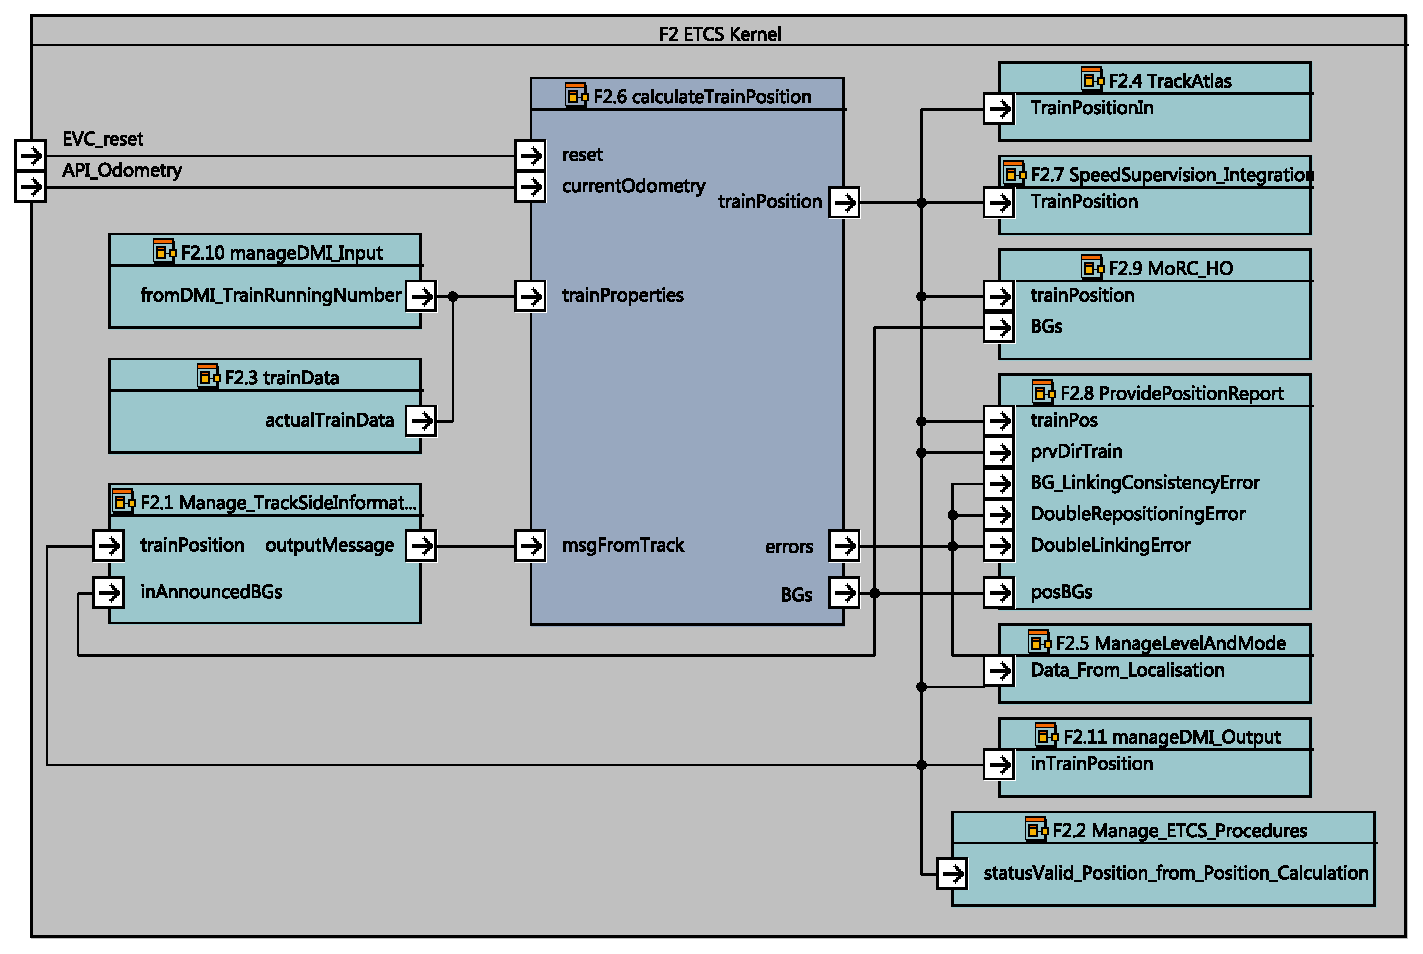
\includegraphics[width=\textwidth]{F2_F2_6.pdf}
\caption{F2: ETCS Kernel SysML diagram with focus on F2.6 calculateTrainPosition component.}\label{f:f2.6_overview}
\end{figure}

\item[F2.7: SpeedSupervision\_Integration] This component monitors the current speed of the train and its location to ensure that the speed remains within the given speed and distance limits. The corresponding SysML diagram is shown in Figure~\ref{f:f2.7_overview}. For further details we refer to Section~\ref{s:F2.7}.
\begin{figure}
\center
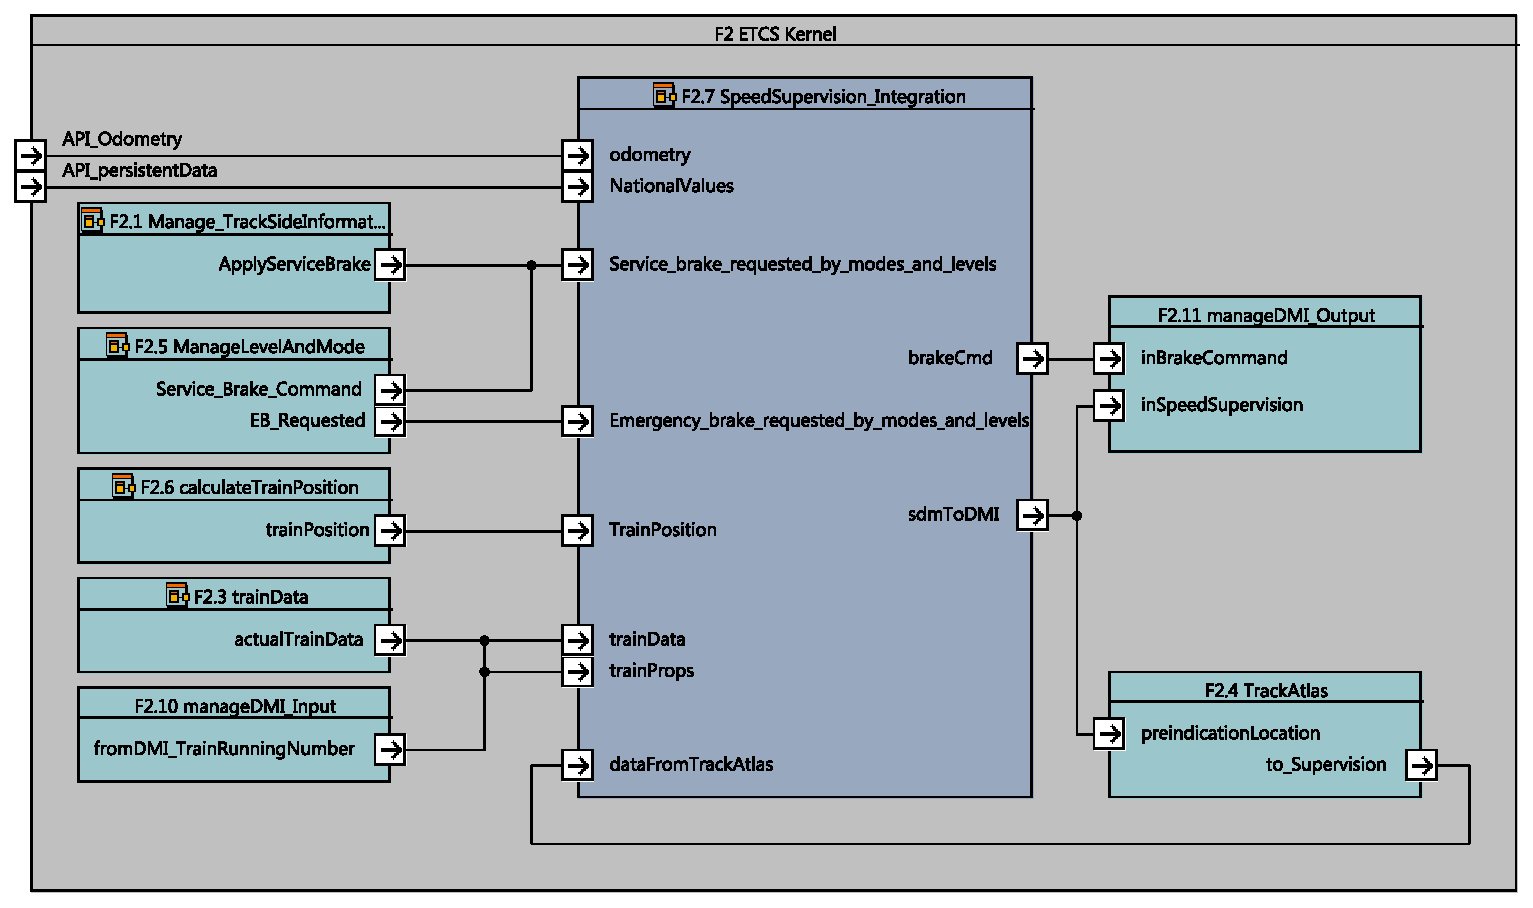
\includegraphics[width=\textwidth]{F2_F2_7.pdf}
\caption{F2: ETCS Kernel SysML diagram with focus on F2.7 SpeedSupervision\_Integration component.}\label{f:f2.7_overview}
\end{figure}

\item[F2.8: Provide\_Position\_Report] The component builds a position report for the RBC, i.e., message 132, and provides it as an output. The corresponding SysML diagram is shown in Figure~\ref{f:f2.8_overview}. For further details we refer to Section~\ref{s:F2.8}.
\begin{figure}
\center
\missingfigure{[Put SysML diagram of component here]}
\caption{F2: ETCS Kernel SysML diagram with focus on F2.8 Provide\_Position\_Report component.}\label{f:f2.8_overview}
\end{figure}

\item[F2.9: Manage\_Radio\_Communication] This component implements the onboard management of a single communication session with the track, i.e.~a single RBC. It controls the establishment, maintenance and termination process of a radio communication session and steers the underlying communication safety layer as well as the mobile device. Those and the data transfer itself are not part of this component. The corresponding SysML diagram is shown in Figure~\ref{f:f2.9_overview}. For further details we refer to Section~\ref{s:F2.9}.
\begin{figure}
\center
\missingfigure{[Put SysML diagram of component here]}
\caption{F2: ETCS Kernel SysML diagram with focus on F2.9 Manage\_Radio\_Communication component.}\label{f:f2.9_overview}
\end{figure}

\item[F2.10: ManageDMIInput] This component handles messages respectively data coming from the Driver Machine Interface (DMI) to the ETCS OBU. The corresponding SysML diagram is shown in Figure~\ref{f:f2.10_overview}. For further details we refer to Section~\ref{s:F2.10}.
\begin{figure}
\center
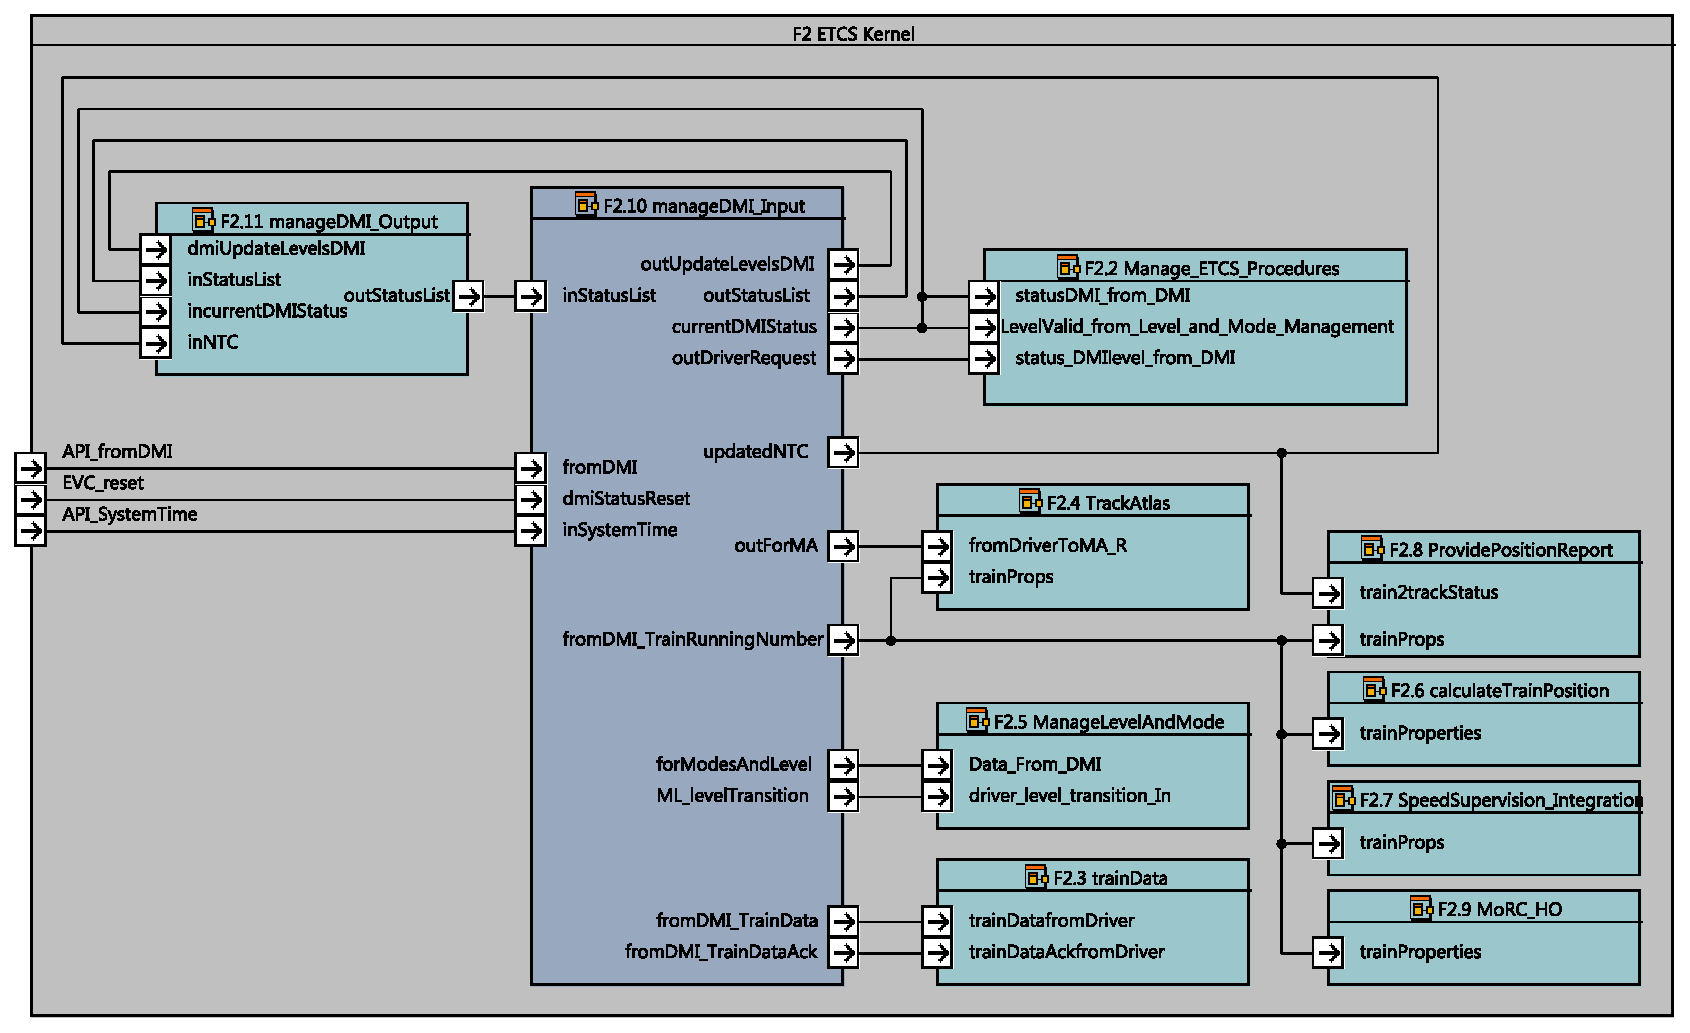
\includegraphics[width=\textwidth]{F2_F2_10.pdf}
\caption{F2: ETCS Kernel SysML diagram with focus on F2.10 ManageDMIInput component.}\label{f:f2.10_overview}
\end{figure}

\item[F2.11: ManageDMIOutput] This component handles messages respectively data being send from the ETCS OBU to the DMI. The corresponding SysML diagram is shown in Figure~\ref{f:f2.11_overview}. For further details we refer to Section~\ref{s:F2.11}.
\begin{figure}
\center
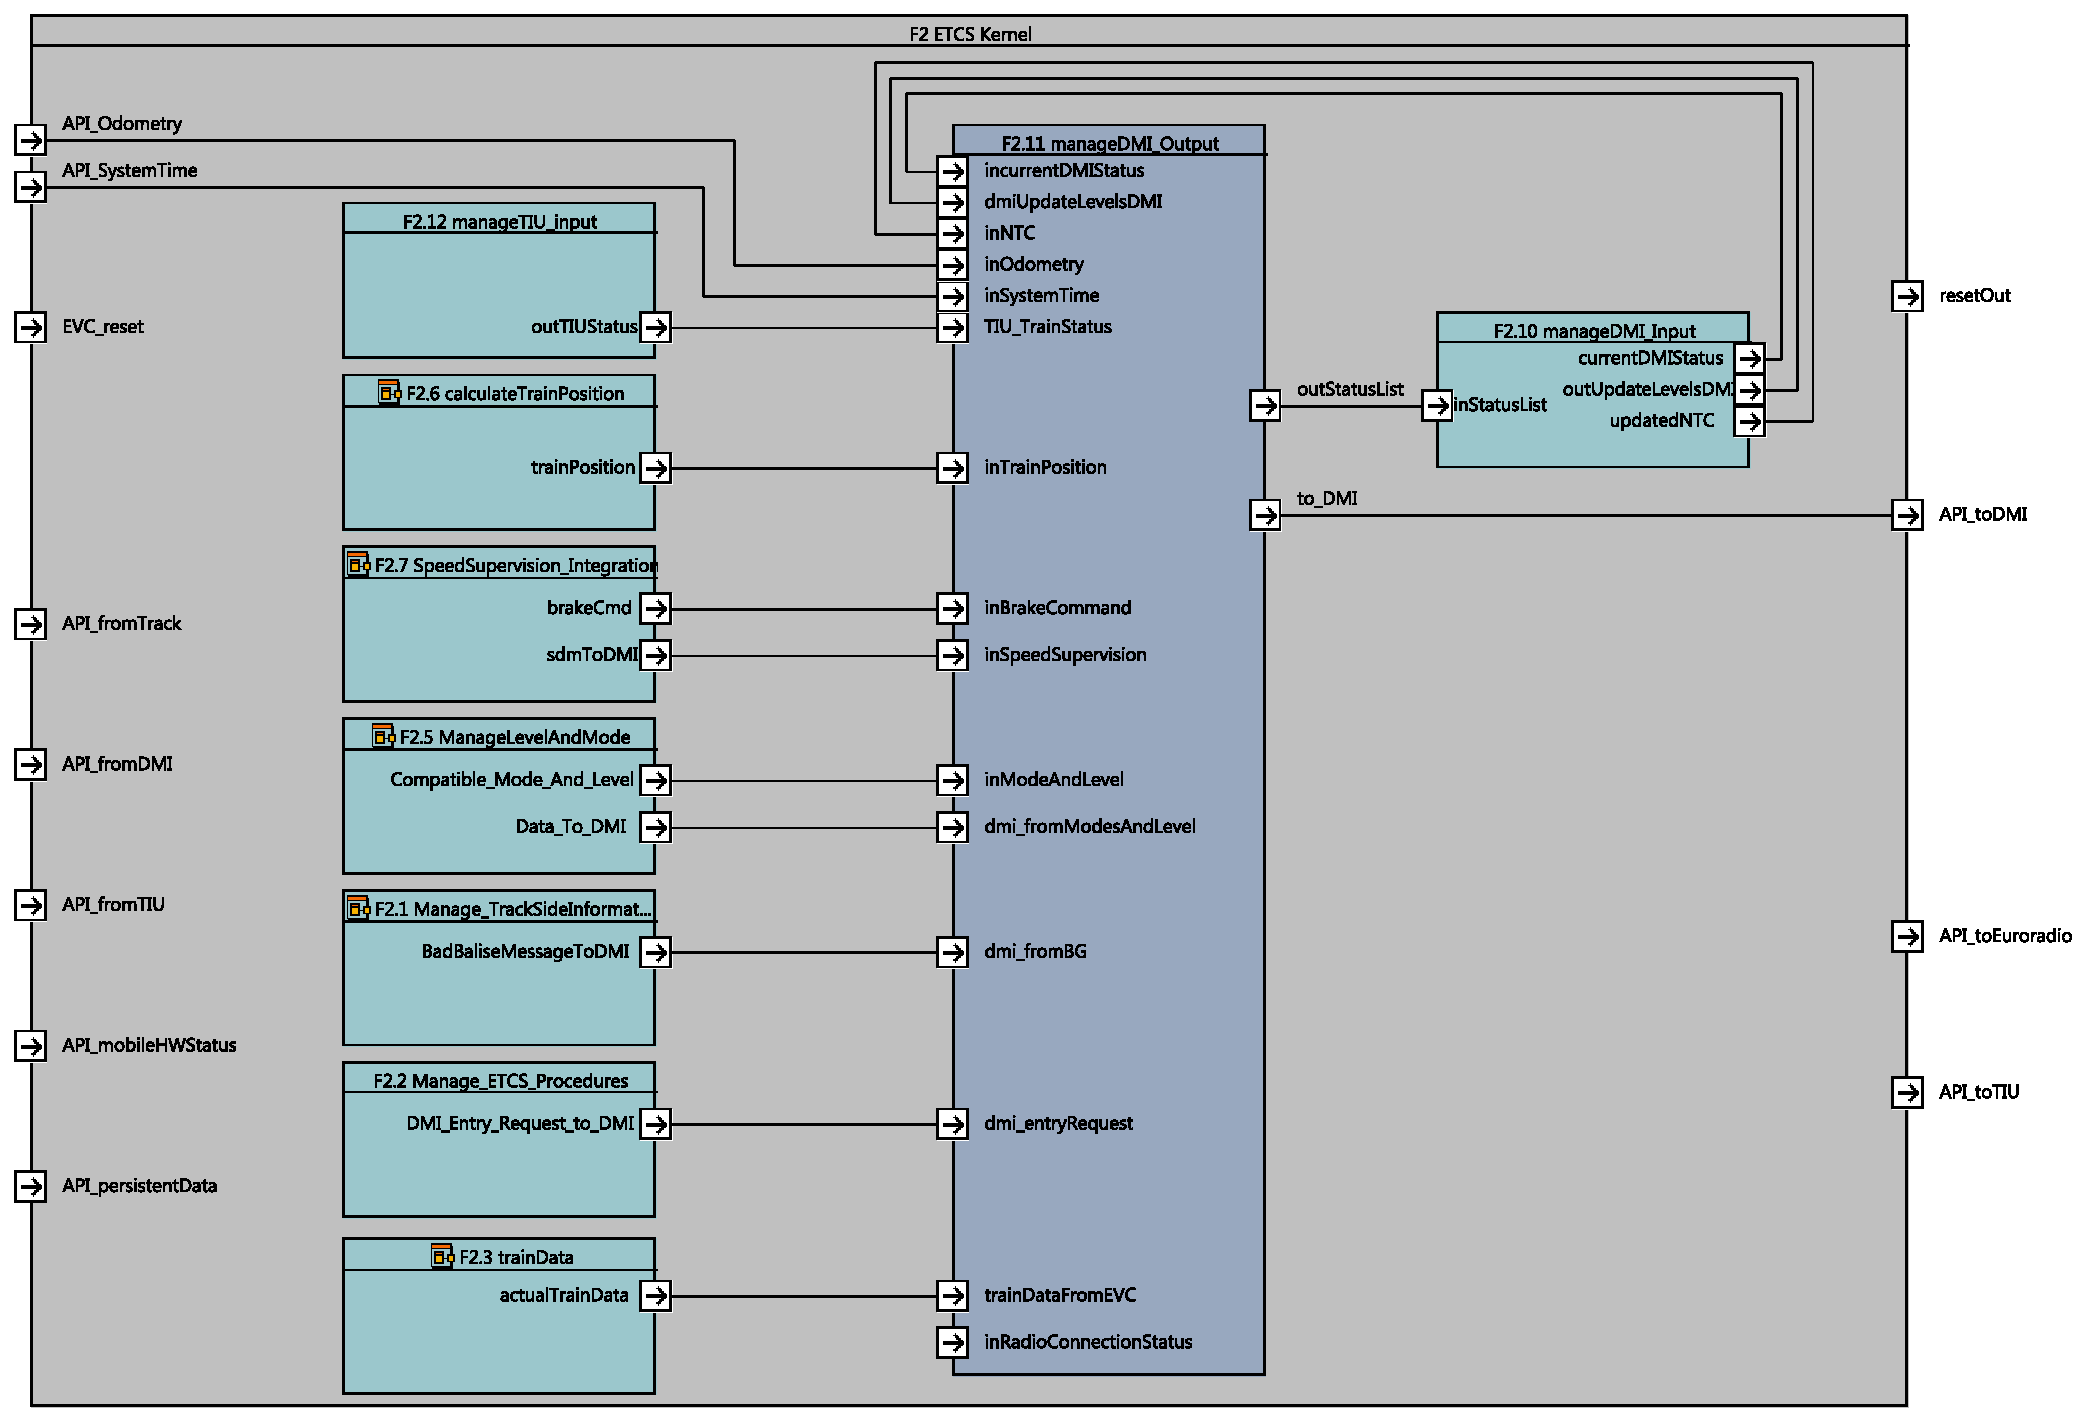
\includegraphics[width=\textwidth]{F2_F2_11.pdf}
\caption{F2: ETCS Kernel SysML diagram with focus on F2.11 ManageDMIOutput component.}\label{f:f2.11_overview}
\end{figure}

\item[F2.12: ManageTIUInput] This component handles messages respectively data coming from the Train Interface Unit (TIU) to the ETCS OBU. The corresponding SysML diagram is shown in Figure~\ref{f:f2.12_overview}. For further details we refer to Section~\ref{s:F2.12}.
\begin{figure}
\center
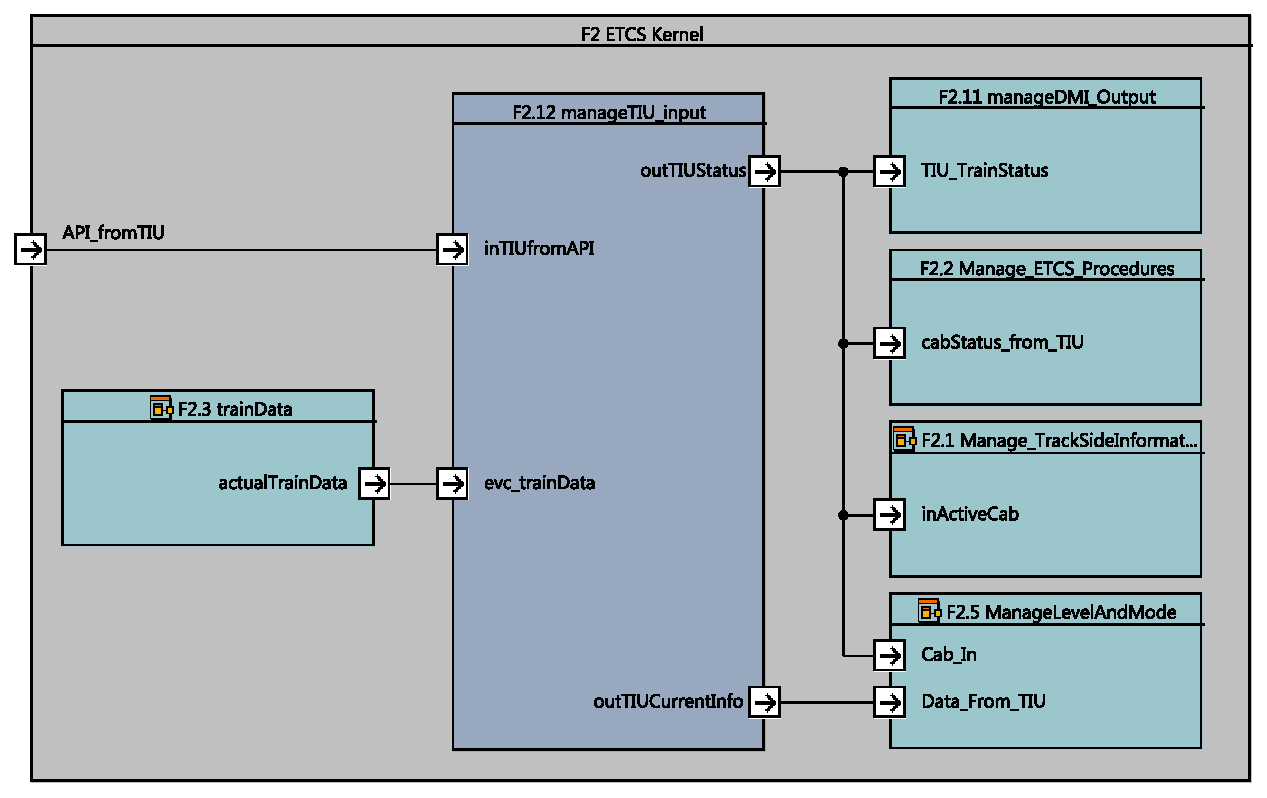
\includegraphics[width=\textwidth]{F2_F2_12.pdf}
\caption{F2: ETCS Kernel SysML diagram with focus on F2.12 ManageTIUInput component.}\label{f:f2.12_overview}
\end{figure}

\item[F2.13: ManageTIUOutput] This component handles messages respectively data being send from the ETCS OBU to the TIU. The corresponding SysML diagram is shown in Figure~\ref{f:f2.13_overview}. For further details we refer to Section~\ref{s:F2.13}.
\begin{figure}
\center
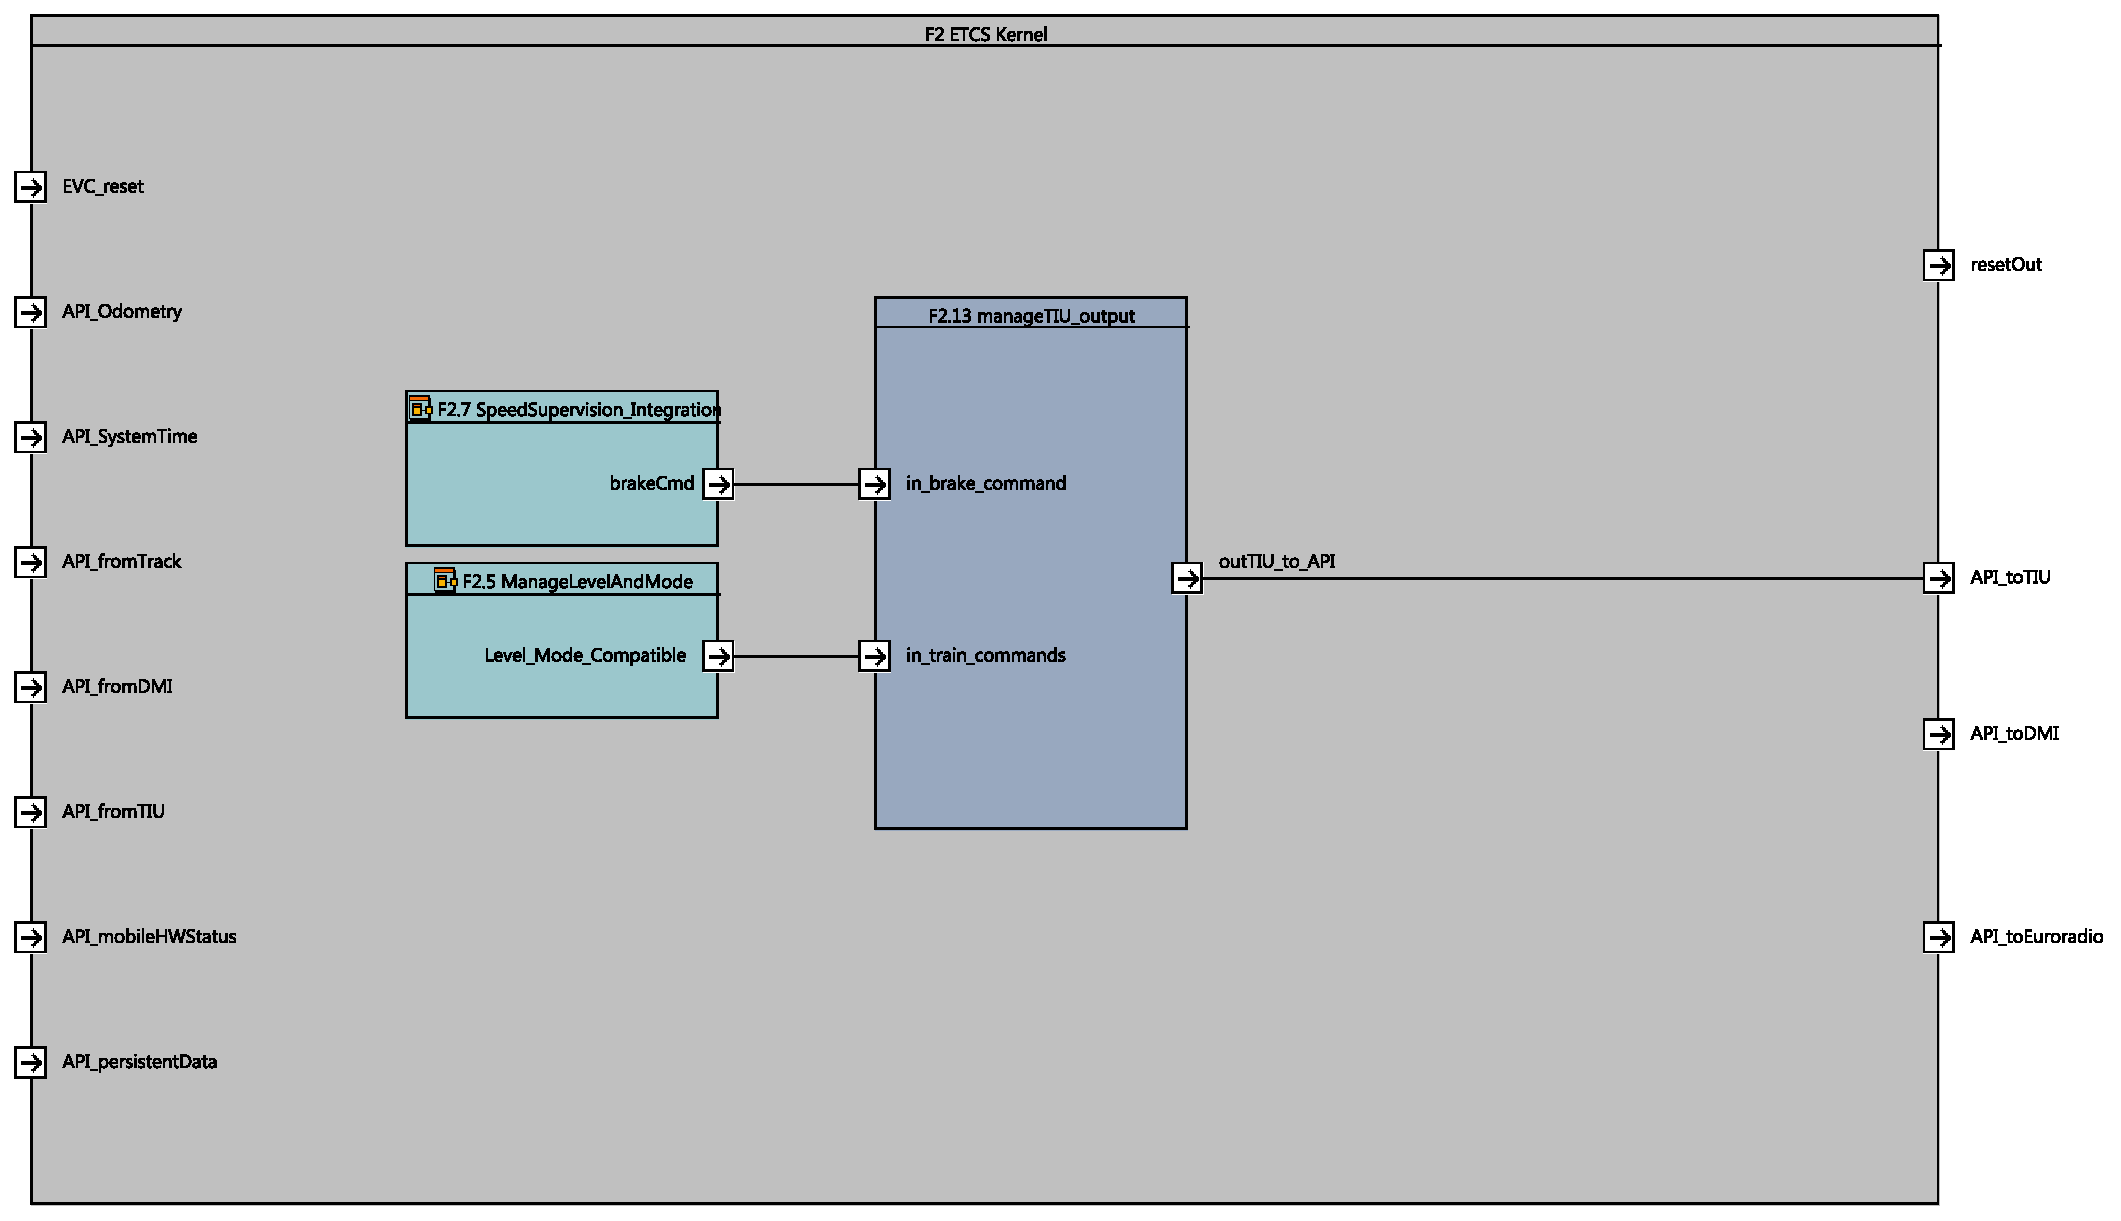
\includegraphics[width=\textwidth]{F2_F2_13.pdf}
\caption{F2: ETCS Kernel SysML diagram with focus on F2.13 ManageTIUOutput component.}\label{f:f2.13_overview}
\end{figure}
\end{description}


\subsection{External Interfaces}
This section gives a detailed overview of the external inputs and outputs of module F2: ETCS Kernel.

\subsubsection{External Inputs}

\paragraph{EVC\_reset}

\begin{longtable}{p{.25\textwidth}p{.7\textwidth}}
\toprule
Input name				& EVC\_reset \\
\midrule
Description				&  The reset input is used to delete all data stored in the connected components inside F2 (e.g.~collected balise telegrams). If the input is set to true, all data kept in the components is deleted and no input is accepted. The reset option is to be used when the EVC is started or in system error scenarios. \\
\midrule
Source					& [Name of the source component] \\ 
\midrule
Type					& [Type of the input] \\
\midrule
Valid range of values	& [Complete list of valid values] \\
\midrule
Behaviour when value is at boundary	& [Description of components behaviour when input value is at boundary] \\
\midrule
Behaviour for values out of valid range	& [Description of components behaviour when input value is out of valid range] \\
\midrule
Behaviour when value is erroneous, absent or unwanted (i.e. spurious) & [Description of components behaviour when value is erroneous, absent or unwanted (i.e. spurious)] \\
\bottomrule
\end{longtable}

\paragraph{API\_Odometry}

\begin{longtable}{p{.25\textwidth}p{.7\textwidth}}
\toprule
Input name				& API\_Odometry \\
\midrule
Description				& Odometry data provided by the external odometry module of the train. \\
\midrule
Source					& API \\ 
\midrule
Type					& [Type of the input] \\
\midrule
Valid range of values	& [Complete list of valid values] \\
\midrule
Behaviour when value is at boundary	& [Description of components behaviour when input value is at boundary] \\
\midrule
Behaviour for values out of valid range	& [Description of components behaviour when input value is out of valid range] \\
\midrule
Behaviour when value is erroneous, absent or unwanted (i.e. spurious) & [Description of components behaviour when value is erroneous, absent or unwanted (i.e. spurious)] \\
\bottomrule
\end{longtable}

\paragraph{API\_SystemTime}

\begin{longtable}{p{.25\textwidth}p{.7\textwidth}}
\toprule
Input name				& API\_SystemTime \\
\midrule
Description				& [Brief description of the input] \\
\midrule
Source					& API \\ 
\midrule
Type					& [Type of the input] \\
\midrule
Valid range of values	& [Complete list of valid values] \\
\midrule
Behaviour when value is at boundary	& [Description of components behaviour when input value is at boundary] \\
\midrule
Behaviour for values out of valid range	& [Description of components behaviour when input value is out of valid range] \\
\midrule
Behaviour when value is erroneous, absent or unwanted (i.e. spurious) & [Description of components behaviour when value is erroneous, absent or unwanted (i.e. spurious)] \\
\bottomrule
\end{longtable}

\paragraph{API\_fromTrack}

\begin{longtable}{p{.25\textwidth}p{.7\textwidth}}
\toprule
Input name				& API\_fromTrack \\
\midrule
Description				& [Brief description of the input] \\
\midrule
Source					& API respectively F1 Receive Information from Trackside\\ 
\midrule
Type					& [Type of the input] \\
\midrule
Valid range of values	& [Complete list of valid values] \\
\midrule
Behaviour when value is at boundary	& [Description of components behaviour when input value is at boundary] \\
\midrule
Behaviour for values out of valid range	& [Description of components behaviour when input value is out of valid range] \\
\midrule
Behaviour when value is erroneous, absent or unwanted (i.e. spurious) & [Description of components behaviour when value is erroneous, absent or unwanted (i.e. spurious)] \\
\bottomrule
\end{longtable}

\paragraph{API\_fromDMI}

\begin{longtable}{p{.25\textwidth}p{.7\textwidth}}
\toprule
Input name				& API\_fromDMI \\
\midrule
Description				& [Brief description of the input] \\
\midrule
Source					& API respectively F6 DMI Controller\\ 
\midrule
Type					& [Type of the input] \\
\midrule
Valid range of values	& [Complete list of valid values] \\
\midrule
Behaviour when value is at boundary	& [Description of components behaviour when input value is at boundary] \\
\midrule
Behaviour for values out of valid range	& [Description of components behaviour when input value is out of valid range] \\
\midrule
Behaviour when value is erroneous, absent or unwanted (i.e. spurious) & [Description of components behaviour when value is erroneous, absent or unwanted (i.e. spurious)] \\
\bottomrule
\end{longtable}

\paragraph{API\_fromTIU}

\begin{longtable}{p{.25\textwidth}p{.7\textwidth}}
\toprule
Input name				& API\_fromTIU \\
\midrule
Description				& [Brief description of the input] \\
\midrule
Source					& API respectively F7 Manage TIU Interface \\ 
\midrule
Type					& [Type of the input] \\
\midrule
Valid range of values	& [Complete list of valid values] \\
\midrule
Behaviour when value is at boundary	& [Description of components behaviour when input value is at boundary] \\
\midrule
Behaviour for values out of valid range	& [Description of components behaviour when input value is out of valid range] \\
\midrule
Behaviour when value is erroneous, absent or unwanted (i.e. spurious) & [Description of components behaviour when value is erroneous, absent or unwanted (i.e. spurious)] \\
\bottomrule
\end{longtable}

\paragraph{API\_mobileHWStatus}

\begin{longtable}{p{.25\textwidth}p{.7\textwidth}}
\toprule
Input name				& API\_mobileHWStatus \\
\midrule
Description				& [Brief description of the input] \\
\midrule
Source					& [Name of the source component] \\ 
\midrule
Type					& [Type of the input] \\
\midrule
Valid range of values	& [Complete list of valid values] \\
\midrule
Behaviour when value is at boundary	& [Description of components behaviour when input value is at boundary] \\
\midrule
Behaviour for values out of valid range	& [Description of components behaviour when input value is out of valid range] \\
\midrule
Behaviour when value is erroneous, absent or unwanted (i.e. spurious) & [Description of components behaviour when value is erroneous, absent or unwanted (i.e. spurious)] \\
\bottomrule
\end{longtable}

\paragraph{API\_persistentData}

\begin{longtable}{p{.25\textwidth}p{.7\textwidth}}
\toprule
Input name				& API\_persistentData \\
\midrule
Description				& [Brief description of the input] \\
\midrule
Source					& [Name of the source component] \\ 
\midrule
Type					& [Type of the input] \\
\midrule
Valid range of values	& [Complete list of valid values] \\
\midrule
Behaviour when value is at boundary	& [Description of components behaviour when input value is at boundary] \\
\midrule
Behaviour for values out of valid range	& [Description of components behaviour when input value is out of valid range] \\
\midrule
Behaviour when value is erroneous, absent or unwanted (i.e. spurious) & [Description of components behaviour when value is erroneous, absent or unwanted (i.e. spurious)] \\
\bottomrule
\end{longtable}



\subsubsection{External Outputs}

\paragraph{resetOut}

\begin{longtable}{p{.25\textwidth}p{.7\textwidth}}
\toprule
Output name				& resetOut \\
\midrule
Description				& [Brief description of the output] \\
\midrule
Destination				& [Name of the destination component(s)] \\ 
\midrule
Type					& [Type of the output] \\
\midrule
Valid range of values	& [Complete list of valid values] \\
\midrule
Behaviour when value is at boundary	& [Description of components behaviour when output value is at boundary] \\
\midrule
Behaviour for values out of valid range	& [Description of components behaviour when output value is out of valid range] \\
\midrule
Behaviour when value is erroneous, absent or unwanted (i.e. spurious) & [Description of components behaviour when value is erroneous, absent or unwanted (i.e. spurious)] \\
\bottomrule
\end{longtable}


\paragraph{API\_toEuroradio}

\begin{longtable}{p{.25\textwidth}p{.7\textwidth}}
\toprule
Output name				& API\_toEuroradio \\
\midrule
Description				& [Brief description of the output] \\
\midrule
Destination				& [Name of the destination component(s)] \\ 
\midrule
Type					& [Type of the output] \\
\midrule
Valid range of values	& [Complete list of valid values] \\
\midrule
Behaviour when value is at boundary	& [Description of components behaviour when output value is at boundary] \\
\midrule
Behaviour for values out of valid range	& [Description of components behaviour when output value is out of valid range] \\
\midrule
Behaviour when value is erroneous, absent or unwanted (i.e. spurious) & [Description of components behaviour when value is erroneous, absent or unwanted (i.e. spurious)] \\
\bottomrule
\end{longtable}


\paragraph{API\_toDMI}

\begin{longtable}{p{.25\textwidth}p{.7\textwidth}}
\toprule
Output name				& API\_toDMI \\
\midrule
Description				& [Brief description of the output] \\
\midrule
Destination				& API respectively F6DMI Controller \\ 
\midrule
Type					& [Type of the output] \\
\midrule
Valid range of values	& [Complete list of valid values] \\
\midrule
Behaviour when value is at boundary	& [Description of components behaviour when output value is at boundary] \\
\midrule
Behaviour for values out of valid range	& [Description of components behaviour when output value is out of valid range] \\
\midrule
Behaviour when value is erroneous, absent or unwanted (i.e. spurious) & [Description of components behaviour when value is erroneous, absent or unwanted (i.e. spurious)] \\
\bottomrule
\end{longtable}

\paragraph{API\_toTIU}

\begin{longtable}{p{.25\textwidth}p{.7\textwidth}}
\toprule
Output name				& API\_toTIU \\
\midrule
Description				& [Brief description of the output] \\
\midrule
Destination				& API respectively F7 Manage TIU Interface \\ 
\midrule
Type					& [Type of the output] \\
\midrule
Valid range of values	& [Complete list of valid values] \\
\midrule
Behaviour when value is at boundary	& [Description of components behaviour when output value is at boundary] \\
\midrule
Behaviour for values out of valid range	& [Description of components behaviour when output value is out of valid range] \\
\midrule
Behaviour when value is erroneous, absent or unwanted (i.e. spurious) & [Description of components behaviour when value is erroneous, absent or unwanted (i.e. spurious)] \\
\bottomrule
\end{longtable}

%set the master document for easy compilation
%!TEX root = ../D3_5_2.tex

\section{Manage\_TrackSideInformation\_Integration}

\subsection{Component Requirements}

\todo{Clarify detail f documentation with the trackMessages concept}


\begin{longtable}{p{.25\textwidth}p{.7\textwidth}}
\toprule
Component name			& Manage\_TrackSideInformation\_Integration \\
\midrule
Link to SCADE model		& {\footnotesize \url{https://github.com/openETCS/modeling/blob/master/model/Scade/System/ObuFunctions/ManageLocationRelatedInformation/BaliseGroup/Manage_TrackSideInformation_Integration/Manage_TrackSideInformation_Integration.etp}} \\
\midrule
SCADE designer			& Bernd Hekele, DB Netz AG \\
\midrule
Description				& The block ``Manage\_TrackSideInformation\_Integration'' is responsible for receiving Eurobalise telegrams and Euroradio messages from the API and performs several consistency checks on the inputs.\newline

The block collects the telegrams of balises in order to build balise group messages. Euroradio messages are always delivered as a whole message. On each message, a consistency check is performed, before the data is validated according to the driving direction of the train. In general, messages not designated for the current driving direction of the train are not forwarded to the further processing. After applying consistency checks, the data direction is validated. \\
\midrule
Input documents	& 
See sub-components.\\
\midrule
Safety integrity level		& 4 \\
\midrule
Time constraints		& The component has to be able to receive balise telegrams and radio messages according to the ETCS \cite{subset-41} performance requirements). In highspeed traffic, a group of 8 balises must be read in about 250 msec. In addition, 1 message per sec. on the radio interface is to be expected.\\
\midrule
API requirements 		& Interfaces to this unit are defined in the API sections [BTM], [EURORADIO], [ODO].In these sections, also a detailed definition of the concepts implemented on those interfaces is documented.  \\
\bottomrule
\end{longtable}


\subsection{Interface}

An overview of the interface of component Manage\_TrackSideInformation\_Integration is shown in Figure~\ref{f:receiveAndCheckConsistencyArch}. The inputs and outputs are described in detail in Section~\ref{s:Manage_Trackside_inputs} respectively \ref{s:Manage_Trackside_outputs}. Sub components are described in Section~\ref{s:receivetrackdata_subcomponents}.

\begin{figure}
\center
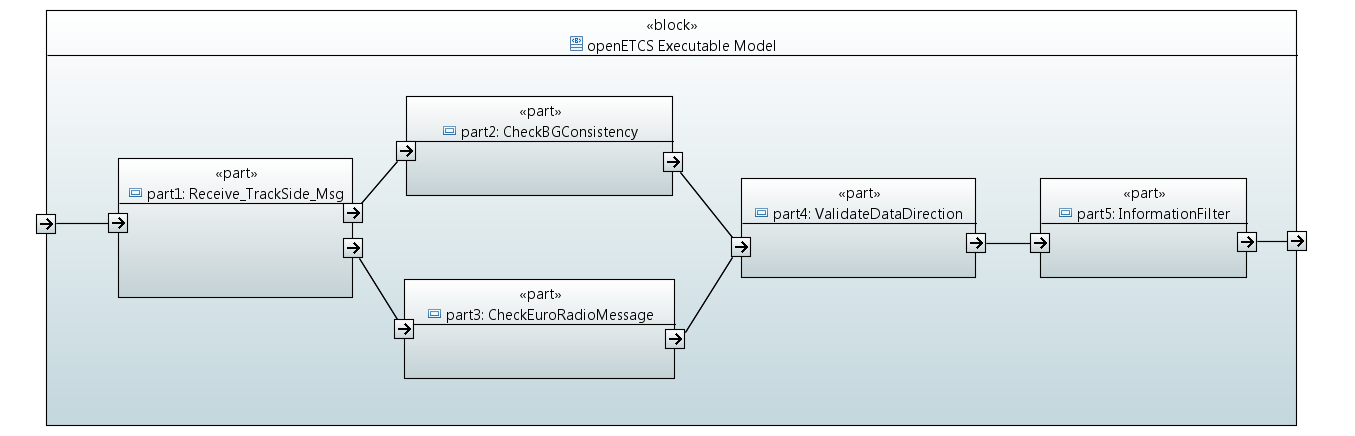
\includegraphics[width=\textwidth]{./images/Input-Messages4.PNG}
\caption{Manage\_TrackSideInformation\_Integration component SysML diagram.}\label{f:receiveAndCheckConsistencyArch}
\end{figure}


\subsubsection{Inputs}\label{s:Manage_Trackside_inputs}

\paragraph{fullChecks}

\begin{longtable}{p{.25\textwidth}p{.7\textwidth}}
\toprule
Input name				& fullChecks \\
\midrule
Description				& Indicates, if all checks on the message should be performed. \\
\midrule
Source					& This item is only relevant in verification phases. In a real system checks are always activated. \\ 
\midrule
Type					& bool \\
\midrule
Valid range of values	& 
\begin{description}
\item[true] All checks are performed.
\item[false] Component InformationFilter is deactivated.
\end{description} \\
\midrule
Behaviour when value is at boundary	& n/a \\
\midrule
Behaviour for values out of valid range	& n/a \\
\midrule
Behaviour when value is erroneous, absent or unwanted (i.e. spurious) & [Description of components behaviour when value is erroneous, absent or unwanted (i.e. spurious)] \\
\bottomrule
\end{longtable}


\paragraph{Receive\_trackSide\_Message}

\begin{longtable}{p{.25\textwidth}p{.7\textwidth}}
\toprule
Input name				& API\_trackSide\_Message \\
\midrule
Description				& Track side message received from the API. The API performs preprocessing of RTM and BTM messages and deliveres a maximum of a single message per cycle. The structure of this message is defined in the API [BTM] and [EURORADIO] sections.\\
\midrule
Source					& API \\ 
\midrule
Type					& API\_Msg\_Pkg::API\_TrackSideInput\_T \\
\midrule
Valid range of values	& [Complete list of valid values] \\
\midrule
Behaviour when value is at boundary	& [Description of components behaviour when input value is at boundary] \\
\midrule
Behaviour for values out of valid range	& [Description of components behaviour when input value is out of valid range] \\
\midrule
Behaviour when value is erroneous, absent or unwanted (i.e. spurious) & [Description of components behaviour when value is erroneous, absent or unwanted (i.e. spurious)] \\
\bottomrule
\end{longtable}


\paragraph{ActualOdometry}

\begin{longtable}{p{.25\textwidth}p{.7\textwidth}}
\toprule
Input name				& ActualOdometry \\
\midrule
Description				& Provided by the external odometry module of the train. It contains relative location information with inaccuracies. \\
\midrule
Source					& Odometer \\ 
\midrule
Type					& Obu\_BasicTypes\_Pkg::odometry\_T \\
\midrule
Valid range of values	& [Complete list of valid values] \\
\midrule
Behaviour when value is at boundary	& [Description of components behaviour when input value is at boundary] \\
\midrule
Behaviour for values out of valid range	& [Description of components behaviour when input value is out of valid range] \\
\midrule
Behaviour when value is erroneous, absent or unwanted (i.e. spurious) & [Description of components behaviour when value is erroneous, absent or unwanted (i.e. spurious)] \\
\bottomrule
\end{longtable}

\paragraph{reset}

\begin{longtable}{p{.25\textwidth}p{.7\textwidth}}
\toprule
Input name				& reset \\
\midrule
Description				& To delete all data stored in the module (e.g.~collected balise telegrams, which do not yet form a complete message), a reset input can be used. If the input is set to true, all data kept in the module is deleted and no input is accepted. \\
\midrule
Source					& Environment \\ 
\midrule
Type					& bool \\
\midrule
Valid range of values	& 
\begin{description}
\item[true] All data kept in the module is deleted and no input is accepted.
\item[false] No action. Data at input is accepted.
\end{description} \\
\midrule
Behaviour when value is at boundary	& [Description of components behaviour when input value is at boundary] \\
\midrule
Behaviour for values out of valid range	& [Description of components behaviour when input value is out of valid range] \\
\midrule
Behaviour when value is erroneous, absent or unwanted (i.e. spurious) & [Description of components behaviour when value is erroneous, absent or unwanted (i.e. spurious)] \\
\bottomrule
\end{longtable}

\paragraph{trainPosition}

\begin{longtable}{p{.25\textwidth}p{.7\textwidth}}
\toprule
Input name				& trainPosition \\
\midrule
Description				& Contains the current position of the train. \\
\midrule
Source					& CalculateTrainPosition \\ 
\midrule
Type					& TrainPosition\_Types\_Pck::trainPosition\_T \\
\midrule
Valid range of values	& \\
\midrule
Behaviour when value is at boundary	& [Description of components behaviour when input value is at boundary] \\
\midrule
Behaviour for values out of valid range	& [Description of components behaviour when input value is out of valid range] \\
\midrule
Behaviour when value is erroneous, absent or unwanted (i.e. spurious) & [Description of components behaviour when value is erroneous, absent or unwanted (i.e. spurious)] \\
\bottomrule
\end{longtable}

\paragraph{modeAndLevel}

\begin{longtable}{p{.25\textwidth}p{.7\textwidth}}
\toprule
Input name				& modeAndLevel \\
\midrule
Description				& Provides the current level and mode of the EVC. \\
\midrule
Source					& ModeAndLevel \\ 
\midrule
Type					& BG\_Types\_Pkg::ModeAndLevelStatus\_T \\
\midrule
Valid range of values	& [Complete list of valid values] \\
\midrule
Behaviour when value is at boundary	& [Description of components behaviour when input value is at boundary] \\
\midrule
Behaviour for values out of valid range	& [Description of components behaviour when input value is out of valid range] \\
\midrule
Behaviour when value is erroneous, absent or unwanted (i.e. spurious) & [Description of components behaviour when value is erroneous, absent or unwanted (i.e. spurious)] \\
\bottomrule
\end{longtable}


\paragraph{tNvContact}

\begin{longtable}{p{.25\textwidth}p{.7\textwidth}}
\toprule
Input name				& tNvContact \\
\midrule
Description				& For monitoring the safe radio connection, this national value is needed as an input. \\
\midrule
Source					& Database \\ 
\midrule
Type					& Obu\_BasicTypes\_Pkg::T\_internal\_Type \\
\midrule
Valid range of values	& [Complete list of valid values] \\
\midrule
Behaviour when value is at boundary	& [Description of components behaviour when input value is at boundary] \\
\midrule
Behaviour for values out of valid range	& [Description of components behaviour when input value is out of valid range] \\
\midrule
Behaviour when value is erroneous, absent or unwanted (i.e. spurious) & [Description of components behaviour when value is erroneous, absent or unwanted (i.e. spurious)] \\
\bottomrule
\end{longtable}


\paragraph{lastRelevantEventTimestamp}

\begin{longtable}{p{.25\textwidth}p{.7\textwidth}}
\toprule
Input name				& lastRelevantEventTimestamp \\
\midrule
Description				& For monitoring the safe radio connection, it is necessary that the time between two packets is less than the value of {T\_NVCONTACT}.\newline
In situations like level-changes or announced radio holes, not the timestamp of the last message is relevant for comparison, but the timestamp of the last relevant event. This can for example be the timestamp of the level change or the timestamp of the moment, when the train was passing the end of the radiohole.\newline
For performing this check, the timestamp of the last relevant event is provided to the model as an {T\_internal\_Type}-type. \\
\midrule
Source					& Database \\ 
\midrule
Type					& Obu\_BasicTypes\_Pkg::T\_internal\_Type \\
\midrule
Valid range of values	& [Complete list of valid values] \\
\midrule
Behaviour when value is at boundary	& [Description of components behaviour when input value is at boundary] \\
\midrule
Behaviour for values out of valid range	& [Description of components behaviour when input value is out of valid range] \\
\midrule
Behaviour when value is erroneous, absent or unwanted (i.e. spurious) & [Description of components behaviour when value is erroneous, absent or unwanted (i.e. spurious)] \\
\bottomrule
\end{longtable}


\paragraph{connectionStatus}

\begin{longtable}{p{.25\textwidth}p{.7\textwidth}}
\toprule
Input name				& connectionStatus \\
\midrule
Description				& Status information about the radio connection. The information is needed to perform the timing check, which depends on the connection state. \\
\midrule
Source					& ManageRadioCommunication \\ 
\midrule
Type					& Radio\_Types\_Pkg::sessionStatus\_Type \\
\midrule
Valid range of values	& 
\begin{description}
\item[DISCONNECTED] The OBU is currently not connected to a RBC.
\item[CONNECTING] The OBU is currently connecting to the RBC. Received messages belong to the process of establishing a connection.
\item[CONNECTION\_ESTABLISHED] The connection to the RBC is established.
\end{description} \\
\midrule
Behaviour when value is at boundary	& [Description of components behaviour when input value is at boundary] \\
\midrule
Behaviour for values out of valid range	& [Description of components behaviour when input value is out of valid range] \\
\midrule
Behaviour when value is erroneous, absent or unwanted (i.e. spurious) & [Description of components behaviour when value is erroneous, absent or unwanted (i.e. spurious)] \\
\bottomrule
\end{longtable}


\paragraph{inSupervisingRbcId}

\begin{longtable}{p{.25\textwidth}p{.7\textwidth}}
\toprule
Input name				& inSupervisingRbcId \\
\midrule
Description				& For the sub component InformationFilter, the information which radio messages are sent by the supervising RBC is needed. To recognize these messages, the identifier of the supervising RBC is needed. \\
\midrule
Source					& Database \\ 
\midrule
Type					& int \\
\midrule
Valid range of values	& [Complete list of valid values] \\
\midrule
Behaviour when value is at boundary	& [Description of components behaviour when input value is at boundary] \\
\midrule
Behaviour for values out of valid range	& [Description of components behaviour when input value is out of valid range] \\
\midrule
Behaviour when value is erroneous, absent or unwanted (i.e. spurious) & [Description of components behaviour when value is erroneous, absent or unwanted (i.e. spurious)] \\
\bottomrule
\end{longtable}


\paragraph{inAnnouncedBGs}

\begin{longtable}{p{.25\textwidth}p{.7\textwidth}}
\toprule
Input name				& inAnnouncedBGs \\
\midrule
Description				& Provides information about balise groups which will be passed by the train soon. This information is generated by Calculate Train Position based on the linking information received from trackside. \\
\midrule
Source					& CalculateTrainPosition \\ 
\midrule
Type					& TrainPosition\_Types\_Pck::positionedBGs\_T \\
\midrule
Valid range of values	& [Complete list of valid values] \\
\midrule
Behaviour when value is at boundary	& [Description of components behaviour when input value is at boundary] \\
\midrule
Behaviour for values out of valid range	& [Description of components behaviour when input value is out of valid range] \\
\midrule
Behaviour when value is erroneous, absent or unwanted (i.e. spurious) & [Description of components behaviour when value is erroneous, absent or unwanted (i.e. spurious)] \\
\bottomrule
\end{longtable}


\paragraph{q\_nvlocacc}

\begin{longtable}{p{.25\textwidth}p{.7\textwidth}}
\toprule
Input name				& q\_nvlocacc \\
\midrule
Description				& The national value determines the location accuracy. \\
\midrule
Source					& Database \\ 
\midrule
Type					& Q\_NVLOCACC \\
\midrule
Valid range of values	& [Complete list of valid values] \\
\midrule
Behaviour when value is at boundary	& [Description of components behaviour when input value is at boundary] \\
\midrule
Behaviour for values out of valid range	& [Description of components behaviour when input value is out of valid range] \\
\midrule
Behaviour when value is erroneous, absent or unwanted (i.e. spurious) & [Description of components behaviour when value is erroneous, absent or unwanted (i.e. spurious)] \\
\bottomrule
\end{longtable}



\subsubsection{Outputs}\label{s:Manage_Trackside_outputs}

\paragraph{outputMessage}

\begin{longtable}{p{.25\textwidth}p{.7\textwidth}}
\toprule
Output name				& outputMessage \\
\midrule
Description				& Combines both balise and radio messages to one common datatype. This datatype contains all variables and packets, which are possible for the given scenario. \\
\midrule
Destination				& [Name of the destination component(s)] \\ 
\midrule
Type					& Common\_Types\_Pkg::ReceivedMessage\_T \\
\midrule
Valid range of values	& [Complete list of valid values] \\
\midrule
Behaviour when value is at boundary	& [Description of components behaviour when output value is at boundary] \\
\midrule
Behaviour for values out of valid range	& [Description of components behaviour when output value is out of valid range] \\
\midrule
Behaviour when value is erroneous, absent or unwanted (i.e. spurious) & [Description of components behaviour when value is erroneous, absent or unwanted (i.e. spurious)] \\
\bottomrule
\end{longtable}


\paragraph{ApplyServiceBrake}

\begin{longtable}{p{.25\textwidth}p{.7\textwidth}}
\toprule
Output name				& ApplyServiceBrake \\
\midrule
Description				&  Indicates if the balise group the train just passed could not be processed correctly. The check results in the request for a service break. \\
\midrule
Destination				& [Name of the destination component(s)] \\ 
\midrule
Type					& bool \\
\midrule
Valid range of values	& [Complete list of valid values] \\
\midrule
Behaviour when value is at boundary	& [Description of components behaviour when output value is at boundary] \\
\midrule
Behaviour for values out of valid range	& [Description of components behaviour when output value is out of valid range] \\
\midrule
Behaviour when value is erroneous, absent or unwanted (i.e. spurious) & [Description of components behaviour when value is erroneous, absent or unwanted (i.e. spurious)] \\
\bottomrule
\end{longtable}


\paragraph{BadBaliseMessageToDMI}

\begin{longtable}{p{.25\textwidth}p{.7\textwidth}}
\toprule
Output name				& BadBaliseMessageToDMI \\
\midrule
Description				& Information to be passed to the DMI to indicate the reception of a ``bad balise'' to the driver. \\
\midrule
Destination				& DMI \\ 
\midrule
Type					& bool \\
\midrule
Valid range of values	& \begin{description}
\item[true] ???
\item[false] ???
\end{description} \\
\midrule
Behaviour when value is at boundary	& [Description of components behaviour when output value is at boundary] \\
\midrule
Behaviour for values out of valid range	& [Description of components behaviour when output value is out of valid range] \\
\midrule
Behaviour when value is erroneous, absent or unwanted (i.e. spurious) & [Description of components behaviour when value is erroneous, absent or unwanted (i.e. spurious)] \\
\bottomrule
\end{longtable}


\paragraph{errorLinkedBG}

\begin{longtable}{p{.25\textwidth}p{.7\textwidth}}
\toprule
Output name				& errorLinkedBG \\
\midrule
Description				& [Brief description of the output] \\
\midrule
Destination				& [Name of the destination component(s)] \\ 
\midrule
Type					& [Type of the output] \\
\midrule
Valid range of values	& \begin{description}
\item[true] An error in a linked balise group was detected.
\item[false] No error in a linked balise group was detected.
\end{description} \\
\midrule
Behaviour when value is at boundary	& [Description of components behaviour when output value is at boundary] \\
\midrule
Behaviour for values out of valid range	& [Description of components behaviour when output value is out of valid range] \\
\midrule
Behaviour when value is erroneous, absent or unwanted (i.e. spurious) & [Description of components behaviour when value is erroneous, absent or unwanted (i.e. spurious)] \\
\bottomrule
\end{longtable}


\paragraph{errorUnlinkedBG}

\begin{longtable}{p{.25\textwidth}p{.7\textwidth}}
\toprule
Output name				& errorUnlinkedBG \\
\midrule
Description				& [Brief description of the output] \\
\midrule
Destination				& [Name of the destination component(s)] \\ 
\midrule
Type					& bool \\
\midrule
Valid range of values	& \begin{description}
\item[true] An error in a unlinked balise group was detected.
\item[false] No error in a unlinked balise group was detected.
\end{description} \\
\midrule
Behaviour when value is at boundary	& [Description of components behaviour when output value is at boundary] \\
\midrule
Behaviour for values out of valid range	& [Description of components behaviour when output value is out of valid range] \\
\midrule
Behaviour when value is erroneous, absent or unwanted (i.e. spurious) & [Description of components behaviour when value is erroneous, absent or unwanted (i.e. spurious)] \\
\bottomrule
\end{longtable}

\paragraph{passedBG}

\begin{longtable}{p{.25\textwidth}p{.7\textwidth}}
\toprule
Output name				& passedBG \\
\midrule
Description				& Provides the received balise group message in a special format needed by the component CalculateTrainPosition. \\
\midrule
Destination				& [Name of the destination component(s)] \\ 
\midrule
Type					& BG\_Types\_Pkg::passedBG\_T \\
\midrule
Valid range of values	& [Complete list of valid values] \\
\midrule
Behaviour when value is at boundary	& [Description of components behaviour when output value is at boundary] \\
\midrule
Behaviour for values out of valid range	& [Description of components behaviour when output value is out of valid range] \\
\midrule
Behaviour when value is erroneous, absent or unwanted (i.e. spurious) & [Description of components behaviour when value is erroneous, absent or unwanted (i.e. spurious)] \\
\bottomrule
\end{longtable}


\paragraph{outPositionParams}

\begin{longtable}{p{.25\textwidth}p{.7\textwidth}}
\toprule
Output name				& outPositionParams \\
\midrule
Description				& Provides the parameters for the position report in a special format needed by the component ProvidePositionReport. \\
\midrule
Destination				& [Name of the destination component(s)] \\ 
\midrule
Type					& Common\_Types\_Pkg::PositionReportParameter\_T \\
\midrule
Valid range of values	& [Complete list of valid values] \\
\midrule
Behaviour when value is at boundary	& [Description of components behaviour when output value is at boundary] \\
\midrule
Behaviour for values out of valid range	& [Description of components behaviour when output value is out of valid range] \\
\midrule
Behaviour when value is erroneous, absent or unwanted (i.e. spurious) & [Description of components behaviour when value is erroneous, absent or unwanted (i.e. spurious)] \\
\bottomrule
\end{longtable}


\paragraph{outRadioManagement}

\begin{longtable}{p{.25\textwidth}p{.7\textwidth}}
\toprule
Output name				& outRadioManagement \\
\midrule
Description				& Provides the messages for radio session management in a special format needed by the component ManagementOfRadioCommunication. \\
\midrule
Destination				& [Name of the destination component(s)] \\ 
\midrule
Type					& Common\_Types\_Pkg::radioManagementMessage\_T \\
\midrule
Valid range of values	& [Complete list of valid values] \\
\midrule
Behaviour when value is at boundary	& [Description of components behaviour when output value is at boundary] \\
\midrule
Behaviour for values out of valid range	& [Description of components behaviour when output value is out of valid range] \\
\midrule
Behaviour when value is erroneous, absent or unwanted (i.e. spurious) & [Description of components behaviour when value is erroneous, absent or unwanted (i.e. spurious)] \\
\bottomrule
\end{longtable}


\paragraph{radioSequenceError}

\begin{longtable}{p{.25\textwidth}p{.7\textwidth}}
\toprule
Output name				& radioSequenceError \\
\midrule
Description				& [Brief description of the output] \\
\midrule
Destination				& [Name of the destination component(s)] \\ 
\midrule
Type					& bool \\
\midrule
Valid range of values	& \begin{description}
\item[true] A sequence error or a timeout has been detected in the radio message.
\item[false] No error in the radio message sequence was detected.
\end{description} \\
\midrule
Behaviour when value is at boundary	& [Description of components behaviour when output value is at boundary] \\
\midrule
Behaviour for values out of valid range	& [Description of components behaviour when output value is out of valid range] \\
\midrule
Behaviour when value is erroneous, absent or unwanted (i.e. spurious) & [Description of components behaviour when value is erroneous, absent or unwanted (i.e. spurious)] \\
\bottomrule
\end{longtable}


\paragraph{radioMessageConsistencyError}

\begin{longtable}{p{.25\textwidth}p{.7\textwidth}}
\toprule
Output name				& radioMessageConsistencyError \\
\midrule
Description				& [Brief description of the output] \\
\midrule
Destination				& [Name of the destination component(s)] \\ 
\midrule
Type					& bool \\
\midrule
Valid range of values	& \begin{description}
\item[true] A consistency error has been detected in the radio message.
\item[false] No consistency error in the radio message was detected.
\end{description} \\
\midrule
Behaviour when value is at boundary	& [Description of components behaviour when output value is at boundary] \\
\midrule
Behaviour for values out of valid range	& [Description of components behaviour when output value is out of valid range] \\
\midrule
Behaviour when value is erroneous, absent or unwanted (i.e. spurious) & [Description of components behaviour when value is erroneous, absent or unwanted (i.e. spurious)] \\
\bottomrule
\end{longtable}


% Description of sub components
\subsection{Sub Components}\label{s:receivetrackdata_subcomponents}

\subsubsection{Receive\_TrackSide\_Msg}
%set the master document for easy compilation
%!TEX root = ../D3_5_3.tex

\todo[inline]{Responsible developer has to be identified.}
\paragraph{Component Requirements}
\begin{longtable}{p{.25\textwidth}p{.7\textwidth}}
\toprule
Component name			& Receive\_TrackSide\_Msg \\
\midrule
Link to SCADE model		& {\footnotesize \url{https://github.com/openETCS/modeling/tree/master/model/Scade/System/ObuFunctions/ManageLocationRelatedInformation/BaliseGroup/Receive_TrackSide_Msg}} \\
\midrule
SCADE designer			& [Name, affiliation] \\
\midrule
Description				& This function defines the interface of the OBU model to the openETCS generic API for Eurobalise  and Euroradio messages. On the interface, either a valid telegram/message is provided or a telegram/message is indicated which could not be received correct when passing the balise or receiving the radio message. The function passes a balise telegram without major changes of the information to the next entity for collecting the balise group information. This entity collects telegrams received via the interface into Balise Group Information. In case of a radio message, the message is converted to an internal format for further processing and passed without changing the information contained.
\begin{itemize}
\item The decoding of balises is done at the API. Also, packets received via the interface are already transformed into a usable shape.
\item Only packets used inside the current model are passed via the interface.
\item Treatment of Packet 5: Linking Information.
Linking Information is added to the linking array starting from index 0 without gaps. Used elements are marked as valid. Elements are sorted according to the order given by the telegram sequence.
\item Telegrams received as invalid are passed to the ``Check-Function'' to process errors in communication with the track side according to the requirements and in a single place.
Telegrams are added to the telegram array starting from index 0 without gaps. Used elements are marked as valid. Elements are stored according to the order given by the telegram sequence.
\item This function does not process information from the packets. The information is passed to the check without further processing of the values. 
\end{itemize} \\
\midrule
Input documents	&
  Subset-026, Chapter 7 and 8: Definition of the Balise Telegram\newline
  Subset-026, Chapter 4.2.2, 4.2.4, 4.2.9: Interface to the BTM\newline
  Subset-026, Chapter 3.4.1 - 3.4.3, 3.16.2: Handling of Balise Telegrams\newline
  Subset-026, Chapter 3.16.2: Check of the balise group\newline
  Subset-026, Chapter 3.4.2: Determining the orientation\newline
  Subset-026, Chapter 4.5.2 Active Functions Table\newline
  Subset-026, Chapter 8.4.4: Rules for Euroradio messages \\
\midrule
Safety integrity level		& 4 \\
\midrule
Time constraints		& n/a \\
\midrule
API requirements 		& n/a \\
\bottomrule
\end{longtable}


\paragraph{Interface}

For an overview of the interface of this internal component we refer to the SCADE model (cf.~link above) respectively the SCADE generated documentation.

\subsubsection{CheckBGConsistency}
%set the master document for easy compilation
%!TEX root = ../D3_5_3.tex

\paragraph{Component Requirements}

\begin{longtable}{p{.25\textwidth}p{.7\textwidth}}
\toprule
Component name			& CheckBGConsistency \\
\midrule
Link to SCADE model		& {\footnotesize \url{https://github.com/openETCS/modeling/tree/master/model/Scade/System/ObuFunctions/ManageLocationRelatedInformation/BaliseGroup/CheckBGConsistency}} \\
\midrule
SCADE designer			& [Name, affiliation] \\
\midrule
Description				& This function verifies the completeness and correctness of the received messages from balise groups. A message consists of at least a telegram and a maximum of 8 telegrams.
\begin{itemize}
\item A message is still complete and correct, if a telegram is missing (or not decoded or incomplete decoded ), and this telegram is duplicated within the balise group and the duplicating one is correctly read.
\item By more than one telegram, the order of the telegrams must be either ascending (nominal) or descending(reverse).
\item A message is correct, if  all message counters (M MCUNT) do not equal 254 (that means: The telegram never fits any message of the group). A message counter can be equal 255 (that means: The telegram fits with all telegrams of the same balise group) and all other values must be the same.
\end{itemize}
The orientation of the BG will also be calculated in this block. The check, if the message has been received in due time and the right at the right expected location, will be performed in "Calculate Train Position". The checks on the validity of the data in the packets and the validity with respect to the direction of motion will be performed in other modules, e.g. "Validate Data Direction". \\
\midrule
Input documents	& 
Subset-026, Chapter 7 and 8: Definition of the Balise Telegram\newline
Subset-026, Chapter 3.4.1-3, 3.16.2: Handling of Balise Telegrams\newline
Subset-026, Chapter 3.16.2: Check of the balise group\newline
Subset-026, Chapter 4.5.2: Active Functions Table\\
\midrule
Safety integrity level		& 4 \\
\midrule
Time constraints		& n/a \\
\midrule
API requirements 		& n/a \\
\bottomrule
\end{longtable}


\paragraph{Interface}

For an overview of the interface of this internal component we refer to the SCADE model (c.f.~link above) respectively the SCADE generated documentation.

\subsubsection{CheckEuroradioMessage}
%set the master document for easy compilation
%!TEX root = ../D3_5_3.tex

\paragraph{Component Requirements}

\begin{longtable}{p{.25\textwidth}p{.7\textwidth}}
\toprule
Component name			& CheckEuroradioMessage \\
\midrule
Link to SCADE model		& {\footnotesize \url{https://github.com/openETCS/modeling/tree/b9c31ce6fdf702b412bbeab3032a8a4dc7c92e5c/model/Scade/System/ObuFunctions/ManageLocationRelatedInformation/BaliseGroup/CheckEuroRadioMessage}} \\
\midrule
SCADE designer			& Stefan Karg, LEA Railergy \\
\midrule
Description				& The component ``CheckEuroradioMessage'' performs consistency and timing checks on the received radio message. These checks are:
\begin{itemize}
 \item Checking the message sequence.
 \item Check if the message violates timing constraints (T\_NVCONTACT).
 \item Check if all mandatory elements are included.
 \item Check if no elements are included, which are forbidden for the given message id.
\end{itemize}
Messages, which violate one or more of these criteria are marked as invalid in the message header and the component signals the reason for the invalidation via different flags as described in the SCADE model. \\
\midrule
Input documents	& 
  Subset-026, Chapter 3.16\newline
  Subset-026, Chapter 8.4.4\\
\midrule
Safety integrity level		& 4 \\
\midrule
Time constraints		& n/a \\
\midrule
API requirements 		& n/a \\
\bottomrule
\end{longtable}


\paragraph{Interface}

For an overview of the interface of this internal component we refer to the SCADE model (cf.~link above) respectively the SCADE generated documentation.

\subsubsection{ValidateDataDirection}
%set the master document for easy compilation
%!TEX root = ../D3_5_3.tex

\paragraph{Component Requirements}

\begin{longtable}{p{.25\textwidth}p{.7\textwidth}}
\toprule
Component name			& CheckEuroradioMessage \\
\midrule
Link to SCADE model		& {\footnotesize \url{https://github.com/openETCS/modeling/tree/master/model/Scade/System/ObuFunctions/ManageLocationRelatedInformation/BaliseGroup/ValidateDataDirection}} \\
\midrule
SCADE designer			& ??? \\
\midrule
Description				& The component filters an input message in order to mark all elements as invalid, which are not designated for the current driving direction of the train.
\begin{itemize}
 \item The operator contains two processing paths for different message types. Radio messages and balise group messages are handeled in a different way. For validating the data direction of a radio message, the check is performed using the balise group referenced in the radio message header as relevant balise group. For balise group message, the LRBG is used.
 \item The metadata of packets, which are recognized as not valid for the current driving direction, is invalidated.
\end{itemize} \\
\midrule
Input documents	& 
  Subset-026, Chapter 3.6.3 \\
\midrule
Safety integrity level	& 4 \\
\midrule
Time constraints		& n/a \\
\midrule
API requirements 		& n/a \\
\bottomrule
\end{longtable}


\paragraph{Interface}

For an overview of the interface of this internal component we refer to the SCADE model (c.f.~link above) respectively the SCADE generated documentation.

\subsubsection{InformationFilter}
%set the master document for easy compilation
%!TEX root = ../D3_5_3.tex

\paragraph{Component Requirements}

\todo[inline]{Information filter component description needs to be checked, i.e. is the description still up to date? Should more documentation provided for this component in the ADD (please check with Bernd Hekele)?}
\begin{longtable}{p{.25\textwidth}p{.7\textwidth}}
\toprule
Component name			& CheckEuroradioMessage \\
\midrule
Link to SCADE model		& {\footnotesize \url{https://github.com/openETCS/modeling/tree/master/model/Scade/System/ObuFunctions/ManageLocationRelatedInformation/BaliseGroup/InformationFilter}} \\
\midrule
SCADE designer			& Christian Stahl, TWT\newline
Alexander Stante, FhG \\
\midrule
Description				& The filter receives track information (balise and radio) and filters them depending of the mode, level and source of the message. Only messages that pass the filter are valid and should be considered by other ETCS subsystems. Figure~\ref{fig:InformationFilterHighLevel} shows the high\-level decomposition of the functionality. The filter is consists of four  components: FirstFilter, SecondFilter, ThirdFilter and TransitionBuffer.

\begin{description}
\item[FirstFilter] This filter performs filtering of messages
based on the current ETCS level. The decisions taken process is
described via a big decision table which contains rows for every
packet and columns for every ETCS level. This table encodes also if
certain additional information is necessary to filter a message like
pending ETCS Level transitions. Based on this filter packets of an
incoming message is either rejected, accepted or the whole message is
put in the TransitionBuffer. Messages are put in the TransitionBuffer
if there is an announced level transition and the received message is
only valid for the upcoming level.

\item[SecondFilter] The SecondFilter mainly considers messages
that are received via Euroradio. Certain messages are directly
rejected while other may be stored in the TransitionBuffer. The buffer
is used to store messages that are received from non supervising RBCs,
but will be reevaluated after a RBC transition.

\item[ThirdFilter] The last filter is functionally very similiar
the the FirstFilter, however it filters depending on the mode. It also
contains a decision table with rows for every packet but the columns
are modes.

\item[TransitionBuffer] The InformationFilter uses two
TransitionBuffers. One is used to store up to three messages for the
ETCS level transition and the other buffer is used for RBC
transitions. The buffer is designed as a ring buffer and message are
read in FIFO order.
\end{description} \\
\midrule
Input documents	& 
  Subset-026, Chapter 4.8 \\
\midrule
Safety integrity level	& 4 \\
\midrule
Time constraints		& n/a \\
\midrule
API requirements 		& n/a \\
\bottomrule
\end{longtable}

\begin{figure}
\centering
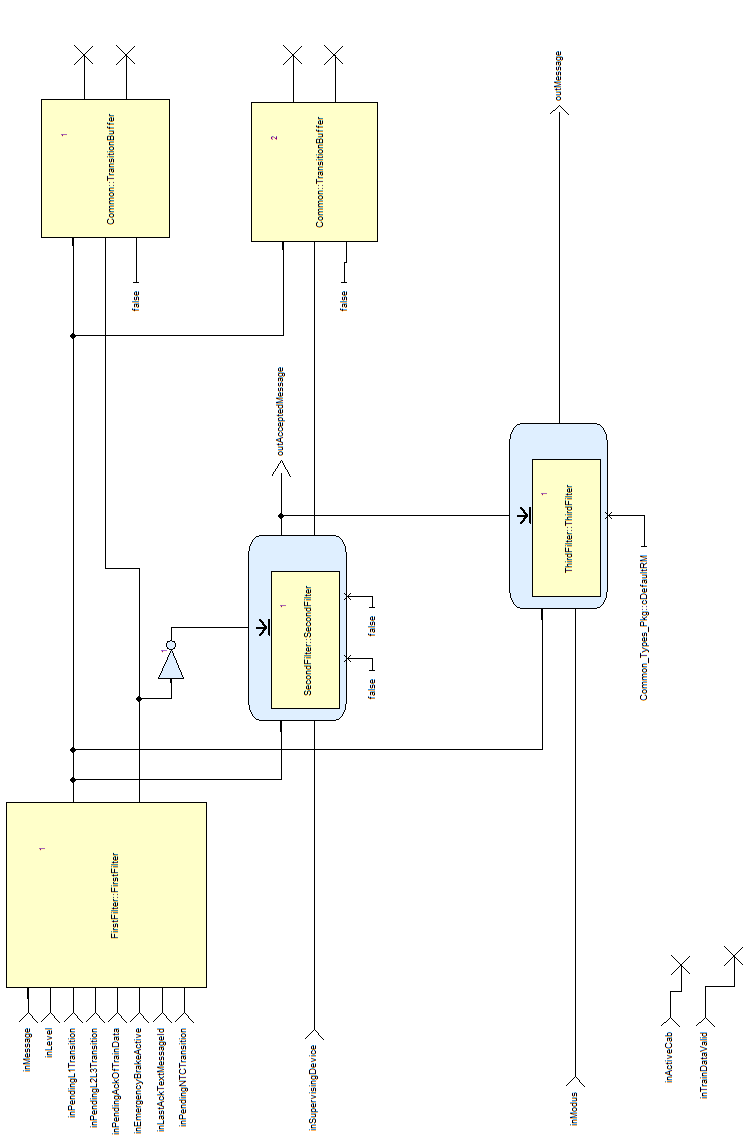
\includegraphics [width=\textwidth]{images/informationfilter-high-level-rot.png}
\caption{High level overview of the InformationFilter components.}
\label{fig:InformationFilterHighLevel}
\end{figure}

\paragraph{Interface}

For an overview of the interface of this internal component we refer to the SCADE model (cf.~link above) respectively the SCADE generated documentation.


%set the master document for easy compilation
%!TEX root = ../D3_5_3.tex

\section{F2.2: Manage\_ETCS\_Procedures}\label{s:F2.2}



\subsection{Component Requirements}

\begin{longtable}{p{.25\textwidth}p{.7\textwidth}}
\toprule
Component name			& Manage\_ETCS\_Procedures \\
\midrule
Link to SCADE model		& {\footnotesize \url{https://github.com/openETCS/modeling/tree/master/model/Scade/System/ObuFunctions/Procedures}} \\
\midrule
SCADE designer			&  Baseliyos Jacob, DB Netz AG\\
\midrule
Description				& This function describes the Start of Mission procedure of the train until the current status will change to another mode, level or other procedure. \\
\midrule
Input documents	& 
Subset-026, Chapter 5.4\\
\midrule
Safety integrity level		& 4 \\
\midrule
Time constraints		& n/a \\
\midrule
API requirements 		& n/a \\
\bottomrule
\end{longtable}


\subsection{Interface}

An overview of the interface of component Manage\_ETCS\_Procedures is shown in Figure~\ref{f:etcs_procedures_interface}. The inputs and outputs are described in detail in Section~\ref{s:etcs_procedures_inputs} respectively \ref{s:etcs_procedures_outputs}. Subcomponents are described in Section~\ref{s:etcs_procedures_subcomponents}.

\begin{figure}
\center
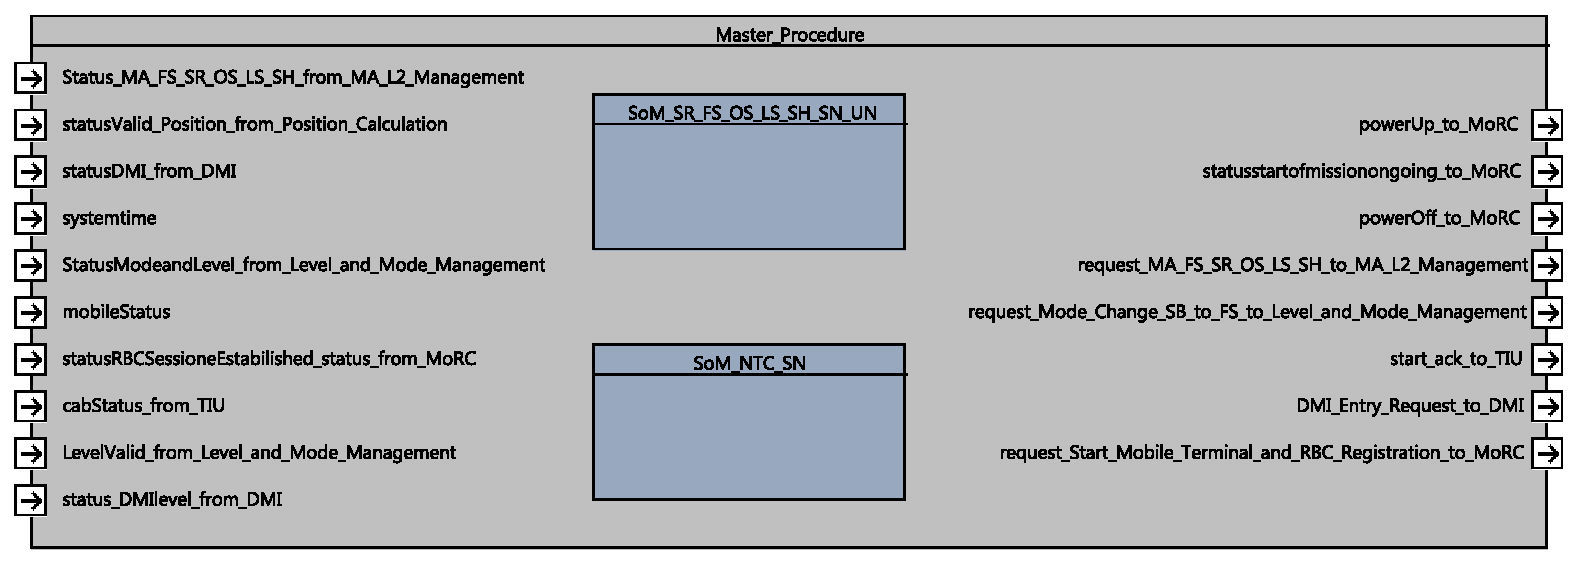
\includegraphics[width=\textwidth]{images/F2_2_Manage_ETCS_Procedures.pdf}
\caption{Manage\_ETCS\_Procedures component SysML diagram.}\label{f:etcs_procedures_interface}
\end{figure}


\subsubsection{Inputs}\label{s:etcs_procedures_inputs}

\paragraph{statusDMI\_from\_DMI}

\begin{longtable}{p{.25\textwidth}p{.7\textwidth}}
\toprule
Input name				& statusDMI\_from\_DMI \\
\midrule
Description				& Input interface of DMI Controller status. \\
\midrule
Source					& F2.10 manageDMI\_input  \\ 
\midrule
Type					& DMI\_Types\_Pkg::DMI\_EVC\_status\_T \\
\midrule
Valid range of values	& See SCADE generated documentation respectively SCADE Suite functional model. \\
\midrule
Behaviour when value is at boundary	& n/a \\
\midrule
Behaviour for values out of valid range	& Function will not be triggered. \\
\midrule
Behaviour when value is erroneous, absent or unwanted (i.e. spurious) & Function will not be triggered. \\
\bottomrule
\end{longtable}


\paragraph{Status\_MA\_FS\_SR\_OS\_LS\_SH\_from\_MA\_L2\_Management}

\begin{longtable}{p{.25\textwidth}p{.7\textwidth}}
\toprule
Input name				& Status\_MA\_FS\_SR\_OS\_LS\_SH\_from\_MA\_L2\_Management \\
\midrule
Description				& Status of MA, Mode and Level from Level and Mode Management. \\
\midrule
Source					& F2.2 Manage\_ETCS\_Procedures \\ 
\midrule
Type					& bool \\
\midrule
Valid range of values	& \begin{description}
\item[true]Movement Authority for Level 2 FS is valid
\item[false]Movement Authority for Level 2 FS is not valid
\end{description} \\
\midrule
Behaviour when value is at boundary	& n/a \\
\midrule
Behaviour for values out of valid range	& n/a \\
\midrule
Behaviour when value is erroneous, absent or unwanted (i.e. spurious) & n/a \\
\bottomrule
\end{longtable}

\paragraph{systemtime}

\begin{longtable}{p{.25\textwidth}p{.7\textwidth}}
\toprule
Input name				& systemtime \\
\midrule
Description				& Standardized system time used for all internal calculations. \\
\midrule
Source					& F2 input API\_Systemtime \\ 
\midrule
Type					& Obu\_BasicTypes\_Pkg::T\_internal\_Type \\
\midrule
Valid range of values	& 
$[0,\text{maximum positive int value of target platform}]$ \\
\midrule
Behaviour when value is at boundary	& System time is assumed to be valid. \\
\midrule
Behaviour for values out of valid range	& System time is assumed to be valid. \\
\midrule
Behaviour when value is erroneous, absent or unwanted (i.e. spurious) & System time is assumed to be valid. \\
\bottomrule
\end{longtable}

\paragraph{StatusModeandLevel\_from\_Level\_and\_Mode\_Management}

\begin{longtable}{p{.25\textwidth}p{.7\textwidth}}
\toprule
Input name				& StatusModeandLevel\_from\_Level\_and\_Mode\_Management  \\
\midrule
Description				& Status of Mode and Level. \\
\midrule
Source					& F2.10 ManageLevelAndMode \\ 
\midrule
Type					& Level\_And\_Mode\_Types\_Pkg::T\_Mode\_Level \\
\midrule
Valid range of values	& See SCADE generated documentation respectively SCADE Suite functional model. \\
\midrule
Behaviour when value is at boundary	& n/a \\
\midrule
Behaviour for values out of valid range	& n/a \\
\midrule
Behaviour when value is erroneous, absent or unwanted (i.e. spurious) & n/a \\
\bottomrule
\end{longtable}

\paragraph{mobileSwStatus\_p\_from\_MoRC}

\begin{longtable}{p{.25\textwidth}p{.7\textwidth}}
\toprule
Input name				& mobileSwStatus\_p\_from\_MoRC  \\
\midrule
Description				& Information about SW status from Management of Radio Communication function. \\
\midrule
Source					& F2.9 MoRC\_HO\\ 
\midrule
Type					& MoRC\_Pck::mobileSWStatus\_Type \\
\midrule
Valid range of values	& See SCADE generated documentation respectively SCADE Suite functional model. \\
\midrule
Behaviour when value is at boundary	&n/a \\
\midrule
Behaviour for values out of valid range	& n/a \\
\midrule
Behaviour when value is erroneous, absent or unwanted (i.e. spurious) & n/a \\
\bottomrule
\end{longtable}

\paragraph{statusRBCSessioneEstabilished\_status\_from\_MoRC}

\begin{longtable}{p{.25\textwidth}p{.7\textwidth}}
\toprule
Input name				& statusRBCSessioneEstabilished\_status\_from\_MoRC  \\
\midrule
Description				& Information about RBC Session status from the Management of Radio Communication function. \\
\midrule
Source					&  F2.9 MoRC\_HO\\ 
\midrule
Type					& Radio\_Types\_Pkg::sessionStatus\_Type \\
\midrule
Valid range of values	& See SCADE generated documentation respectively SCADE Suite functional model. \\
\midrule
Behaviour when value is at boundary	& n/a \\
\midrule
Behaviour for values out of valid range	& n/a \\
\midrule
Behaviour when value is erroneous, absent or unwanted (i.e. spurious) & n/a \\
\bottomrule
\end{longtable}

\paragraph{cabStatus\_from\_TIU}

\begin{longtable}{p{.25\textwidth}p{.7\textwidth}}
\toprule
Input name				& cabStatus\_from\_TIU  \\
\midrule
Description				& Information about cab desk status from Train Interface Unit function. \\
\midrule
Source					& F2.12 manageTIU\_input\\ 
\midrule
Type					& TIU\_Types\_Pkg::TIU\_trainStatus\_T \\
\midrule
Valid range of values	& See SCADE generated documentation respectively SCADE Suite functional model. \\
\midrule
Behaviour when value is at boundary	& n/a \\
\midrule
Behaviour for values out of valid range	& n/a \\
\midrule
Behaviour when value is erroneous, absent or unwanted (i.e. spurious) & n/a \\
\bottomrule
\end{longtable}

\paragraph{statusValid\_Position\_from\_Position\_Calculation}

\begin{longtable}{p{.25\textwidth}p{.7\textwidth}}
\toprule
Input name				& statusValid\_Position\_from\_Position\_Calculation  \\
\midrule
Description				& Information about validity status of the train position calculation. \\
\midrule
Source					& F2.6 calculateTrainPosition\\ 
\midrule
Type					& bool \\
\midrule
Valid range of values	& \begin{description}
\item[true]Calculated train position is valid.
\item[false]Calculated train position is not valid.
\end{description} \\
\midrule
Behaviour when value is at boundary	& n/a \\
\midrule
Behaviour for values out of valid range	& n/a\\
\midrule
Behaviour when value is erroneous, absent or unwanted (i.e. spurious) & n/a \\
\bottomrule
\end{longtable}

\paragraph{status\_DMIlevel\_from\_DMI}

\begin{longtable}{p{.25\textwidth}p{.7\textwidth}}
\toprule
Input name				& status\_DMIlevel\_from\_DMI  \\
\midrule
Description				& Information about the status of DMI menu and level request from DMIController function. \\
\midrule
Source					& F2.10 manageDMI\_input\\ 
\midrule
Type					& DMI\_Messages\_DMI\_to\_EVC\_Pkg::DMI\_Driver\_Request\_T \\
\midrule
Valid range of values	& See SCADE generated documentation respectively SCADE Suite functional model. \\
\midrule
Behaviour when value is at boundary	& n/a \\
\midrule
Behaviour for values out of valid range	& n/a \\
\midrule
Behaviour when value is erroneous, absent or unwanted (i.e. spurious) & n/a \\
\bottomrule
\end{longtable}

\paragraph{LevelValid\_from\_Level\_and\_Mode\_Management}

\begin{longtable}{p{.25\textwidth}p{.7\textwidth}}
\toprule
Input name				& LevelValid\_from\_Level\_and\_Mode\_Management  \\
\midrule
Description				& Information about the validty status of  the StatusModeandLevel\_from\_Level\_and\_Mode\_Management input. \\
\midrule
Source					& F2.5 ManageModeAndLevel \\
\midrule
Type					& bool \\
\midrule
Valid range of values	& \begin{description}
\item[true]Level and Mode information are valid.
\item[false]Level and Mode information are not valid.
\end{description} \\
\midrule
Behaviour when value is at boundary	& n/a \\
\midrule
Behaviour for values out of valid range	& n/a\\
\midrule
Behaviour when value is erroneous, absent or unwanted (i.e. spurious) & n/a \\
\bottomrule
\end{longtable}

\subsubsection{Outputs}\label{s:etcs_procedures_outputs}

\paragraph{DMI\_Entry\_Request\_to\_DMI}

\begin{longtable}{p{.25\textwidth}p{.7\textwidth}}
\toprule
Output name				& DMI\_Entry\_Request\_to\_DMI \\
\midrule
Description				& Information about input request to the driver. \\
\midrule
Destination				& F2.11 manageDMI\_output \\ 
\midrule
Type					& DMI\_Messages\_EVC\_to\_DMI\_Pkg::DMI\_Entry\_Request\_T \\
\midrule
Valid range of values	& See SCADE generated documentation respectively SCADE Suite functional model. \\
\midrule
Behaviour when value is at boundary	& n/a \\
\midrule
Behaviour for values out of valid range	& n/a \\
\midrule
Behaviour when value is erroneous, absent or unwanted (i.e. spurious) & n/a \\
\bottomrule
\end{longtable}

\paragraph{request\_Start\_Mobile\_Terminal\_and\_RBC\_Registration\_to\_MoRC}

\begin{longtable}{p{.25\textwidth}p{.7\textwidth}}
\toprule
Output name				& request\_Start\_Mobile\_Terminal\_and\_RBC\_Registration\_to\_MoRC \\
\midrule
Description				& This output is a trigger to start the mobile terminal and RBC session registration within the Management of Radio Communication function. \\
\midrule
Destination				& F2.9 MoRC\_HI \\
\midrule
Type					& Common\_Types\_Pkg::radioManagementMessage\_T \\
\midrule
Valid range of values	& See SCADE generated documentation respectively SCADE Suite functional model. \\
\midrule
Behaviour when value is at boundary	& n/a \\
\midrule
Behaviour for values out of valid range	& n/A \\
\midrule
Behaviour when value is erroneous, absent or unwanted (i.e. spurious) & n/a \\
\bottomrule
\end{longtable}

\paragraph{powerUp\_to\_MoRC}

\begin{longtable}{p{.25\textwidth}p{.7\textwidth}}
\toprule
Output name				& powerUp\_to\_MoRC \\
\midrule
Description				& This output is the trigger to activate the Management of Radio Communication function. \\
\midrule
Destination				& F2.9 MoRC\_HO \\ 
\midrule
Type					& bool \\
\midrule
Valid range of values	& \begin{description}
\item[true]MoRC will be activated. 
\item[false]No action.
\end{description} \\
\midrule
Behaviour when value is at boundary	& n/a \\
\midrule
Behaviour for values out of valid range	& n/a \\
\midrule
Behaviour when value is erroneous, absent or unwanted (i.e. spurious) & n/a \\
\bottomrule
\end{longtable}

\paragraph{statusstartofmissionongoing\_to\_MoRC}

\begin{longtable}{p{.25\textwidth}p{.7\textwidth}}
\toprule
Output name				& statusstartofmissionongoing\_to\_MoRC \\
\midrule
Description				& This output gives the information about the start of mission status procedure to the Management of Radio Communication function. \\
\midrule
Destination				& F2.9 MoRC\_HO \\ 
\midrule
Type					& bool \\
\midrule
Valid range of values	& \begin{description}
\item[true]Start of mission procedure is currently ongoing.
\item[false]Start of mission procedure is currently not ongoing.
\end{description} \\
\midrule
Behaviour when value is at boundary	& n/a \\
\midrule
Behaviour for values out of valid range	& n/a \\
\midrule
Behaviour when value is erroneous, absent or unwanted (i.e. spurious) & n/a \\
\bottomrule
\end{longtable}

\paragraph{powerOff\_to\_MoRC}

\begin{longtable}{p{.25\textwidth}p{.7\textwidth}}
\toprule
Output name				& powerOff\_to\_MoRC \\
\midrule
Description				& This output is the trigger to de-activate the Management of Radio Communication function. \\
\midrule
Destination				& F2.9 MoRC\_HO \\ 
\midrule
Type					& bool \\
\midrule
Valid range of values	& \begin{description}
\item[true]MoRC will be deactivated. 
\item[false]no action.
\end{description} \\
\midrule
Behaviour when value is at boundary	& n/a \\
\midrule
Behaviour for values out of valid range	& n/a \\
\midrule
Behaviour when value is erroneous, absent or unwanted (i.e. spurious) & n/a \\
\bottomrule
\end{longtable}

\paragraph{start\_ack\_to\_TIU}

\begin{longtable}{p{.25\textwidth}p{.7\textwidth}}
\toprule
Output name				& start\_ack\_to\_TIU \\
\midrule
Description				& This output indicates that the start of mission procedure is completed. \\
\midrule
Destination				& Output is currently not used in the model. \\ 
\midrule
Type					& bool \\
\midrule
Valid range of values	&  \begin{description}
\item[true]Start of mission procedure is completed.
\item[false]Not defined. 
\end{description} \\
\midrule
Behaviour when value is at boundary	& n/a \\
\midrule
Behaviour for values out of valid range	& n/a \\
\midrule
Behaviour when value is erroneous, absent or unwanted (i.e. spurious) & n/a \\
\bottomrule
\end{longtable}


\subsection{Subcomponents}\label{s:etcs_procedures_subcomponents}

\subsubsection{Awakness\_of\_Train}
%set the master document for easy compilation
%!TEX root = ../D3_5_3.tex

\paragraph{Component Requirements}

\begin{longtable}{p{.25\textwidth}p{.7\textwidth}}
\toprule
Component name			& Awakness\_of\_Train \\
\midrule
Link to SCADE model		& {\footnotesize \url{https://github.com/openETCS/modeling/blob/master/model/Scade/System/ObuFunctions/Procedures/ManageProcedure_Pkg.xscade}} \\
\midrule
SCADE designer			& Baseliyos Jacob, DB Netz AG \\
\midrule
Description				& This component describes the Start of Mission procedure of the train until the status of the awakening is completed. From this point on the train will be able to switch to further modes, levels and procedures. \\

\midrule
Input documents	& 
Subset-026, Chapter 5, § 5.4 \\
\midrule
Safety integrity level		& 4 \\
\midrule
Time constraints		& n/a \\
\midrule
API requirements 		& n/a \\
\bottomrule
\end{longtable}



\paragraph{Interface}

For an overview of the interface of this internal component we refer to the SCADE model (cf.~link above) respectively the SCADE generated documentation.

\subsubsection{NP}
%set the master document for easy compilation
%!TEX root = ../D3_5_3.tex

\paragraph{Component Requirements}

\begin{longtable}{p{.25\textwidth}p{.7\textwidth}}
\toprule
Component name			& NP \\
\midrule
Link to SCADE model		& {\footnotesize \url{https://github.com/openETCS/modeling/blob/master/model/Scade/System/ObuFunctions/Procedures/ManageProcedure_Pkg.xscade}} \\
\midrule
SCADE designer			& Baseliyos Jacob, DB Netz AG \\
\midrule
Description				& This component implements the No Power status of the train before the driver opens the cab desk. \\

\midrule
Input documents	& 
Subset-026, Chapter 5, § 5.4 \\
\midrule
Safety integrity level		& 4 \\
\midrule
Time constraints		& n/a \\
\midrule
API requirements 		& n/a \\
\bottomrule
\end{longtable}



\paragraph{Interface}

For an overview of the interface of this internal component we refer to the SCADE model (c.f.~link above) respectively the SCADE generated documentation.

\subsubsection{SoM\_L2\_3\_FS\_SR\_OS\_LS\_SH}
%set the master document for easy compilation
%!TEX root = ../D3_5_3.tex

\paragraph{Component Requirements}

\begin{longtable}{p{.25\textwidth}p{.7\textwidth}}
\toprule
Component name			& SoM\_L2\_3\_FS\_SR\_OS\_LS\_SH \\
\midrule
Link to SCADE model		& {\footnotesize \url{https://github.com/openETCS/modeling/blob/master/model/Scade/System/ObuFunctions/Procedures/ManageProcedure_Pkg.xscade}} \\
\midrule
SCADE designer			& Baseliyos Jacob, DB Netz AG \\
\midrule
Description				& This component switch to Level 2 or 3 and Mode FS, SR, OS, LS and SH after completion of the awakening of the train. \\

\midrule
Input documents	& 
Subset-026, Chapter 5, § 5.4 \\
\midrule
Safety integrity level		& 4 \\
\midrule
Time constraints		& n/a \\
\midrule
API requirements 		& n/a \\
\bottomrule
\end{longtable}



\paragraph{Interface}

For an overview of the interface of this internal component we refer to the SCADE model (c.f.~link above) respectively the SCADE generated documentation.

\subsubsection{SoM\_NTC\_SN}
%set the master document for easy compilation
%!TEX root = ../D3_5_3.tex

\paragraph{Component Requirements}

\begin{longtable}{p{.25\textwidth}p{.7\textwidth}}
\toprule
Component name			& SoM\_NTC\_SN \\
\midrule
Link to SCADE model		& {\footnotesize \url{https://github.com/openETCS/modeling/blob/master/model/Scade/System/ObuFunctions/Procedures/ManageProcedure_Pkg.xscade}} \\
\midrule
SCADE designer			& Baseliyos Jacob, DB Netz AG \\
\midrule
Description				& This component switch to Level NTC and Mode SN after completion of the awakening of the train. \\

\midrule
Input documents	& 
Subset-026, Chapter 5, § 5.4 \\
\midrule
Safety integrity level		& 4 \\
\midrule
Time constraints		& n/a \\
\midrule
API requirements 		& n/a \\
\bottomrule
\end{longtable}



\paragraph{Interface}

For an overview of the interface of this internal component we refer to the SCADE model (c.f.~link above) respectively the SCADE generated documentation.




%set the master document for easy compilation
%!TEX root = ../D3_5_3.tex

\section{F2.3: trainData}

\subsection{Component Requirements}

\begin{longtable}{p{.25\textwidth}p{.7\textwidth}}
\toprule
Component name			& trainData \\
\midrule
Link to SCADE model		& {\footnotesize \url{https://github.com/openETCS/modeling/blob/master/model/Scade/System/ObuFunctions/manageData/trainData/trainData.etp}} \\
\midrule
SCADE designer			& Bernd Hekele, DB Netz AG \\
\midrule
Description				& Implementation of the train data with the corresponding interfaces to track, driver and RBC.

\todo[inline]{descriptions needs to be improved to be more comprehensive}

Data first is received from the train (TIU).
 
Second step: train data is sent to the driver (DMI).
The part relevant for driver interface is confirmed by the driver and sent back to the EVC.

Data received via this interface is merged with the data received via TIU.
Message Flow:
\begin{itemize}
\item sending Message 129 (Validated Train Data)
\item receiving Message 8 (Acknowledment of Train Data) is processed as apart of the validation procedure with the RBC.
\item sending Message 146 (Acknolwedement) in the context of this message flow. T\_TRAIN parameter of the messages is used to confirm the association of the messages.
\end{itemize}

The trainData component uses a dedicated state for controlling the reception of the acknowledgement.\\
\midrule
Input documents	& Subset-026, Chapter 3.18.3\\
\midrule
Safety integrity level	& 4 \\
\midrule
Time constraints		& n/a \\
\midrule
API requirements 		& Train Data needs systemtime for stamping messages, access to input from the track messages and access to the output of RBC messages.\\
\bottomrule
\end{longtable}


\subsection{Interface}

An overview of the interface of component trainData is shown in Figure~\ref{f:traindata_interface}. The inputs and outputs are described in detail in Section~\ref{s:traindata_inputs} respectively \ref{s:traindata_outputs}. Subcomponents are described in Section~\ref{s:traindata_subcomponents}.

\begin{figure}
\center
\missingfigure{[Put SysML diagram of component here]}
\caption{trainData component SysML diagram}\label{f:traindata_interface}
\end{figure}


\subsubsection{Inputs}\label{s:traindata_inputs}

\paragraph{reset}

\begin{longtable}{p{.25\textwidth}p{.7\textwidth}}
\toprule
Input name				& reset \\
\midrule
Description				& Triggers the reset of the train data and the train data status data.\\
\midrule
Source					& Persistant data status management.\\ 
\midrule
Type					& bool \\
\midrule
Valid range of values	& 
\begin{description}
\item[true] Perform reset of train data and train data status.
\item[false] No reset of data in this cycle.
\end{description}
\\
\midrule
Behaviour when value is at boundary	& n/a \\
\midrule
Behaviour for values out of valid range	& n/a \\
\midrule
Behaviour when value is erroneous, absent or unwanted (i.e. spurious) & n/a \\
\bottomrule
\end{longtable}

\paragraph{trainDatafromTIU}

\begin{longtable}{p{.25\textwidth}p{.7\textwidth}}
\toprule
Input name				& trainDatafromTIU \\
\midrule
Description				& Train data received via TIU. The availability of data is indicated with the valid flag. This data is expected to be received in the first place. In the current implementation it is not supported to change data after a mission has been started.\\
\midrule
Source					& Train Interface Unit (TIU) \\ 
\midrule
Type					& TIU\_Types\_Pkg::trainData\_T \\
\midrule
Valid range of values	& Input with valid information is indicated with the valid flag. 
\todo[inline]{Looking at this input this seems to be a complex structure. Consider describing the structure instead of refering to the valid flag only.}\\
\midrule
Behaviour when value is at boundary	& n/a\\
\midrule
Behaviour for values out of valid range	& When valid flag indicates false the data to be used is assumed to be default values. The component is not used when valid flag is false.\\
\midrule
Behaviour when value is erroneous, absent or unwanted (i.e. spurious) & Information is only expected at Start of Mission Procedure. Once the information is successfully received it is not considered any more. Change of train data by train during mission is not supported by this version of the openETCS OBU model.\\
\bottomrule
\end{longtable}

\paragraph{trainDatafromDriver}

\begin{longtable}{p{.25\textwidth}p{.7\textwidth}}
\toprule
Input name				& trainDatafromDriver \\
\midrule
Description				& Train data received via DMI from the driver. The availability of data is indicated with the valid flag. This data is expected to be received in the first place. In the current implementation it is not supported to change data after a mission has been started.\\
\midrule
Source					& Driver Machine Interface (DMI) \\ 
\midrule
Type					& DMI\_Messages\_Bothways\_Pkg::DMI\_Train\_Data\_T \\
\midrule
Valid range of values	& Input with valid information is indicated with the valid flag. 
\todo[inline]{Looking at this input this seems to be a complex structure. Consider describing the structure instead of refering to the valid flag only.}\\
\midrule
Behaviour when value is at boundary	& n/a\\
\midrule
Behaviour for values out of valid range	& When valid flag indicates false the data to be used is assumed to be default values. The component is not used when valid flag is false.\\
\midrule
Behaviour when value is erroneous, absent or unwanted (i.e. spurious) & No checks on individual values is done in this part of the openETCS EVC. We assume - if necessary - appropriate checks are part of the interface layer (e.g., CRC checks) This type of checks is not in the scope of the openETCS project.\\
\bottomrule

\end{longtable}

\paragraph{trainDataAckfromDriver}

\begin{longtable}{p{.25\textwidth}p{.7\textwidth}}
\toprule
Input name				& trainDataAckfromDriver \\
\midrule
Description				& During start of mission the driver has to validate the train data. The confirmation is visible  based on this input. Presence of the input is indicated with the valid flag. 
\todo[inline]{Looking at this input this seems to be a complex structure. Consider describing the structure instead of refering to the valid flag only.}\\
\midrule
Source					& Driver Machine Interface (DMI) \\ 
\midrule
Type					& DMI\_Messages\_DMI\_to\_EVC\_Pkg::DMI\_Train\_Data\_Ack\_T \\
\midrule
Valid range of values	& Input with valid information is indicated with the valid flag. In addition, the ack parameter has to be evaluated in order to recognise the decision of the driver.\\
\midrule
Behaviour when value is at boundary	& n/a\\
\midrule
Behaviour for values out of valid range	& when valid flag indicates false the data to be used is assumed to be default values. The component is not used when valid flag is false.\\
\midrule
Behaviour when value is erroneous, absent or unwanted (i.e. spurious) & no checking on individual values is done in this part of the openETCS EVC. We assume - if necessary - appropriate checks are part of the interface layer (e.g., CRC checks) This type of checks is not in the scope of the openETCS project.\\

\bottomrule
\end{longtable}
\paragraph{trackMessages}

\begin{longtable}{p{.25\textwidth}p{.7\textwidth}}
\toprule
Input name				& trackMessages \\
\midrule
Description				& Information carries the message received from RBC. Information is only used when the valid flag is true and the message source is Radio. Other information is not relevant. Information is evaluated as long as the validation procedure is not completed and a valdiation request with the RBC is pending.\\
\midrule
Source					& Radio Transmission Module (RTM)\\ 
\midrule
Type					& Common\_Types\_Pkg::ReceivedMessage\_T \\
\midrule
Valid range of values	& Input with valid information is indicated with the valid flag.
\todo[inline]{Looking at this input this seems to be a complex structure. Consider describing the structure instead of refering to the valid flag only.}\\
\midrule
Behaviour when value is at boundary	& n/a\\
\midrule
Behaviour for values out of valid range	& 
When valid flag indicates false the data to be used is assumed to be default values. The component is not used when valid flag is false.\\
\midrule
Behaviour when value is erroneous, absent or unwanted (i.e. spurious) & 
No checking on individual values is done in this part of the openETCS EVC. We assume - if necessary - appropriate checks are part of the interface layer (e.g., CRC checks) This type of checks is not in the scope of the openETCS project.\\

\bottomrule
\end{longtable}

\paragraph{timeStamp}

\begin{longtable}{p{.25\textwidth}p{.7\textwidth}}
\toprule
Input name				& timeStamp \\
\midrule
Description				& Timestamp for messaging to the RBC.\\
\midrule
Source					& Derived from train time.\\ 
\midrule
Type					& T\_TRAIN\\
\midrule
Valid range of values	& Positive non-zero real\\
\midrule
Behaviour when value is at boundary	& Parameter is not used for computation or addressing. No impact in this model.\\
\midrule
Behaviour for values out of valid range	& No impact in the EVC. Communication to the RBC will be broken.\\
\midrule
Behaviour when value is erroneous, absent or unwanted (i.e. spurious) & Communication to the RBC will be broken. No safety issue in the EVC since RBC connection errors are covered by the EVC function.
\\
\bottomrule
\end{longtable}


\paragraph{eventsForTrainData}

\begin{longtable}{p{.25\textwidth}p{.7\textwidth}}
\toprule
Input name				& eventsForTrainData\\
\midrule
Description				& Timestamp for messaging to the RBC. Information of the EVC relevant for train data handling according to Section 3.18.3. In the current state of implementation the following events are evaluated:
\begin{itemize}
\item train stand-still
\item communication Session established
\end{itemize}
The MoRC ready input is used to indicate the evc:morc function is ready with acknowledgment of the communication session.\\
\midrule
Source					& EVC model.\\ 
\midrule
Type					& trainData\_Types\_pkg::trainData\_Events\_T\\
\midrule
Valid range of values	& Structure of a set of bool. Each component may be true or false.\\
\midrule
Behaviour when value is at boundary	& n/a\\
\midrule
Behaviour for values out of valid range	& n/a\\
\midrule
Behaviour when value is erroneous, absent or unwanted (i.e. spurious) & n/a\\

\bottomrule
\end{longtable}

\subsubsection{Outputs}\label{s:traindata_outputs}
\todo[inline]{section needs to be completed}
\paragraph{[Output 1 name]}

\begin{longtable}{p{.25\textwidth}p{.7\textwidth}}
\toprule
Output name				& [Name of the output] \\
\midrule
Description				& [Brief description of the output] \\
\midrule
Destination				& [Name of the destination component(s)] \\ 
\midrule
Type					& [Type of the output] \\
\midrule
Valid range of values	& [Complete list of valid values] \\
\midrule
Behaviour when value is at boundary	& [Description of components behaviour when output value is at boundary] \\
\midrule
Behaviour for values out of valid range	& [Description of components behaviour when output value is out of valid range] \\
\midrule
Behaviour when value is erroneous, absent or unwanted (i.e. spurious) & [Description of components behaviour when value is erroneous, absent or unwanted (i.e. spurious)] \\
\bottomrule
\end{longtable}


\paragraph{[Output 2 name]}

\begin{longtable}{p{.25\textwidth}p{.7\textwidth}}
\toprule
Output name				& [Name of the output] \\
\midrule
Description				& [Brief description of the output] \\
\midrule
Destination				& [Name of the destination component(s)] \\ 
\midrule
Type					& [Type of the output] \\
\midrule
Valid range of values	& [Complete list of valid values] \\
\midrule
Behaviour when value is at boundary	& [Description of components behaviour when output value is at boundary] \\
\midrule
Behaviour for values out of valid range	& [Description of components behaviour when output value is out of valid range] \\
\midrule
Behaviour when value is erroneous, absent or unwanted (i.e. spurious) & [Description of components behaviour when value is erroneous, absent or unwanted (i.e. spurious)] \\
\bottomrule
\end{longtable}


\subsection{Subcomponents}\label{s:traindata_subcomponents}

\todo[inline]{section needs to be completed}

\subsubsection{checkRadioMessages}
%set the master document for easy compilation
%!TEX root = ../D3_5_3.tex

\paragraph{Component Requirements}

\begin{longtable}{p{.25\textwidth}p{.7\textwidth}}
\toprule
Component name			& checkRadioMessages \\
\midrule
Link to SCADE model		& {\footnotesize {\url{https://github.com/openETCS/modeling/blob/master/model/Scade/System/ObuFunctions/manageData/trainData/trainData.etp}}} \\
\midrule
SCADE designer			& Bernd Hekele, DB Netz AG \\
\midrule
Description				& The function checks an incoming radio message for relevance in the trainData context. Result is whether the message requests an acknowledgement and whether the radio message is a response to an outstanding validation request.\\
\midrule
Input documents	& 
Subset-026, Chapter 3.18.3\\
\midrule
Safety integrity level	& 4 \\
\midrule
Time constraints		& n/a \\
\midrule
API requirements 		& n/a \\
\bottomrule
\end{longtable}


\paragraph{Interface}

For an overview of the interface of this internal component we refer to the SCADE model (cf.~link above) respectively the SCADE generated documentation.

\subsubsection{checkAcknowledgementGeneral}
%set the master document for easy compilation
%!TEX root = ../D3_5_3.tex

\paragraph{Component Requirements}

\begin{longtable}{p{.25\textwidth}p{.7\textwidth}}
\toprule
Component name			& checkAcknowledgementGeneral \\
\midrule
Link to SCADE model		& {\footnotesize {\url{https://github.com/openETCS/modeling/blob/master/model/Scade/System/ObuFunctions/manageData/trainData/trainData.etp}}} \\
\midrule
SCADE designer			& Bernd Hekele, DB Netz AG \\
\midrule
Description				& This function implements the acknowledment to ma request and general message. It is actually an extension of the trainData function and needs to be moved to radio management functions.\\
\midrule
Input documents	& 
Subset-026, Chapter 3.18.3\\
\midrule
Safety integrity level	& 4 \\
\midrule
Time constraints		& n/a \\
\midrule
API requirements 		& n/a \\
\bottomrule
\end{longtable}


\paragraph{Interface}

For an overview of the interface of this internal component we refer to the SCADE model (cf.~link above) respectively the SCADE generated documentation.

\subsubsection{trainDataStorage}
%set the master document for easy compilation
%!TEX root = ../D3_5_3.tex

\paragraph{Component Requirements}

\begin{longtable}{p{.25\textwidth}p{.7\textwidth}}
\toprule
Component name			& checkAcknowledgementGeneral \\
\midrule
Link to SCADE model		& {\footnotesize {\url{https://github.com/openETCS/modeling/blob/master/model/Scade/System/ObuFunctions/manageData/trainData/trainData.etp}}} \\
\midrule
SCADE designer			& Bernd Hekele, DB Netz AG \\
\midrule
Description				& This function implements the acknowledment to ma request and general message. It is actually an extension of the trainData function and needs to be moved to radio management functions.\\
\midrule
Input documents	& 
Subset-026, Chapter 3.18.3\\
\midrule
Safety integrity level	& 4 \\
\midrule
Time constraints		& n/a \\
\midrule
API requirements 		& n/a \\
\bottomrule
\end{longtable}


\paragraph{Interface}

For an overview of the interface of this internal component we refer to the SCADE model (cf.~link above) respectively the SCADE generated documentation.

\subsubsection{sendAcknowledgementRBC}
%set the master document for easy compilation
%!TEX root = ../D3_5_3.tex

\paragraph{Component Requirements}

\begin{longtable}{p{.25\textwidth}p{.7\textwidth}}
\toprule
Component name			& sendAcknowledgementRBC \\
\midrule
Link to SCADE model		& {\footnotesize {\url{https://github.com/openETCS/modeling/blob/master/model/Scade/System/ObuFunctions/manageData/trainData/trainData.etp}}} \\
\midrule
SCADE designer			& Bernd Hekele, DB Netz AG \\
\midrule
Description				& This function prepares the Information foracknowledgement message .
It is assumed it used with an boolean activator. \\
\midrule
Input documents	& 
Subset-026, Chapter 3.18.3\\
\midrule
Safety integrity level	& 4 \\
\midrule
Time constraints		& n/a \\
\midrule
API requirements 		& n/a \\
\bottomrule
\end{longtable}


\paragraph{Interface}

For an overview of the interface of this internal component we refer to the SCADE model (cf.~link above) respectively the SCADE generated documentation.

\subsubsection{sendValidTrainDataRBC}
%set the master document for easy compilation
%!TEX root = ../D3_5_3.tex

\paragraph{Component Requirements}

\begin{longtable}{p{.25\textwidth}p{.7\textwidth}}
\toprule
Component name			& sendValidTrainDataRBC \\
\midrule
Link to SCADE model		& {\footnotesize {\url{https://github.com/openETCS/modeling/blob/master/model/Scade/System/ObuFunctions/manageData/trainData/trainData.etp}}} \\
\midrule
SCADE designer			& Bernd Hekele, DB Netz AG \\
\midrule
Description				& This function send the validate data request ot the RBC an updates trainData States with the relevant information.\\
\midrule
Input documents	& 
Subset-026, Chapter 3.18.3\\
\midrule
Safety integrity level	& 4 \\
\midrule
Time constraints		& n/a \\
\midrule
API requirements 		& n/a \\
\bottomrule
\end{longtable}


\paragraph{Interface}

For an overview of the interface of this internal component we refer to the SCADE model (cf.~link above) respectively the SCADE generated documentation.




%set the master document for easy compilation
%!TEX root = ../D3_5_3.tex

\section{F2.4: TrackAtlas}
\todo[inline]{Section needs to be completed}

\subsection{Component Requirements}

\begin{longtable}{p{.25\textwidth}p{.7\textwidth}}
\toprule
Component name			& TrackAtlas \\
\midrule
Link to SCADE model		& {\footnotesize \url{???}} \\
\midrule
SCADE designer			& Jakob G\"artner, LEA \\
\midrule
Description				& ??? \\
\midrule
Input documents	& 
Subset-026, Chapter ???\\
\midrule
Safety integrity level	& 4 \\
\midrule
Time constraints		& [If applicable description of time constraints, otherwise n/a] \\
\midrule
API requirements 		& [If applicable description of API requirements, otherwise n/a] \\
\bottomrule
\end{longtable}


\subsection{Interface}

An overview of the interface of component TrackAtlas is shown in Figure~\ref{f:manage_track_data_interface}. The inputs and outputs are described in detail in Section~\ref{s:manage_track_data_inputs} respectively \ref{s:manage_track_data_outputs}. Subcomponents are described in Section~\ref{s:manage_track_data_subcomponents}.

\begin{figure}
\center
\missingfigure{[Put SysML diagram of component here]}
\caption{TrackAtlas component SysML diagram}\label{f:manage_track_data_interface}
\end{figure}


\subsubsection{Inputs}\label{s:manage_track_data_inputs}

\paragraph{[Input 1 name]}

\begin{longtable}{p{.25\textwidth}p{.7\textwidth}}
\toprule
Input name				& [Name of the input] \\
\midrule
Description				& [Brief description of the input] \\
\midrule
Source					& [Name of the source component] \\ 
\midrule
Type					& [Type of the input] \\
\midrule
Valid range of values	& [Complete list of valid values] \\
\midrule
Behaviour when value is at boundary	& [Description of components behaviour when input value is at boundary] \\
\midrule
Behaviour for values out of valid range	& [Description of components behaviour when input value is out of valid range] \\
\midrule
Behaviour when value is erroneous, absent or unwanted (i.e. spurious) & [Description of components behaviour when value is erroneous, absent or unwanted (i.e. spurious)] \\
\bottomrule
\end{longtable}


\paragraph{[Input 2 name]}

\begin{longtable}{p{.25\textwidth}p{.7\textwidth}}
\toprule
Input name				& [Name of the input] \\
\midrule
Description				& [Brief description of the input] \\
\midrule
Source					& [Name of the source component] \\ 
\midrule
Type					& [Type of the input] \\
\midrule
Valid range of values	& [Complete list of valid values] \\
\midrule
Behaviour when value is at boundary	& [Description of components behaviour when input value is at boundary] \\
\midrule
Behaviour for values out of valid range	& [Description of components behaviour when input value is out of valid range] \\
\midrule
Behaviour when value is erroneous, absent or unwanted (i.e. spurious) & [Description of components behaviour when value is erroneous, absent or unwanted (i.e. spurious)] \\
\bottomrule
\end{longtable}


\subsubsection{Outputs}\label{s:manage_track_data_outputs}

\paragraph{[Output 1 name]}

\begin{longtable}{p{.25\textwidth}p{.7\textwidth}}
\toprule
Output name				& [Name of the output] \\
\midrule
Description				& [Brief description of the output] \\
\midrule
Destination				& [Name of the destination component(s)] \\ 
\midrule
Type					& [Type of the output] \\
\midrule
Valid range of values	& [Complete list of valid values] \\
\midrule
Behaviour when value is at boundary	& [Description of components behaviour when output value is at boundary] \\
\midrule
Behaviour for values out of valid range	& [Description of components behaviour when output value is out of valid range] \\
\midrule
Behaviour when value is erroneous, absent or unwanted (i.e. spurious) & [Description of components behaviour when value is erroneous, absent or unwanted (i.e. spurious)] \\
\bottomrule
\end{longtable}


\paragraph{[Output 2 name]}

\begin{longtable}{p{.25\textwidth}p{.7\textwidth}}
\toprule
Output name				& [Name of the output] \\
\midrule
Description				& [Brief description of the output] \\
\midrule
Destination				& [Name of the destination component(s)] \\ 
\midrule
Type					& [Type of the output] \\
\midrule
Valid range of values	& [Complete list of valid values] \\
\midrule
Behaviour when value is at boundary	& [Description of components behaviour when output value is at boundary] \\
\midrule
Behaviour for values out of valid range	& [Description of components behaviour when output value is out of valid range] \\
\midrule
Behaviour when value is erroneous, absent or unwanted (i.e. spurious) & [Description of components behaviour when value is erroneous, absent or unwanted (i.e. spurious)] \\
\bottomrule
\end{longtable}


\subsection{Subcomponents}\label{s:manage_track_data_subcomponents}

\subsubsection{StoreRaw\_NV}
%set the master document for easy compilation
%!TEX root = ../D3_5_3.tex

\paragraph{Component Requirements}

\begin{longtable}{p{.25\textwidth}p{.7\textwidth}}
\toprule
Component name			& StoreRaw\_NV \\
\midrule
Link to SCADE model		& {\footnotesize \url{https://github.com/openETCS/modeling/tree/master/model/Scade/
System/ObuFunctions/TrackAtlas/TA\_Storage}} \\
\midrule
SCADE designer			& Jakob G\"artner, LEA Railergy \\
\midrule
Description				& Receives National Values from the track. Stores them "as-is" onboard. If Subset\_026 chapter 6 is applicable, baseline 3 conformal information is calculated based on packet 3 and packet 203 (according to older versions). Missing trackside information is complemented throug default onboard values. \\
\midrule
Input documents	& 
Subset-026, Chapter 6
Subset-026, Chapter 7
Subset-026, Chapter 8\\
\midrule
Safety integrity level	& 4 \\
\midrule
Time constraints		& n/a \\
\midrule
API requirements 		& Based on data formats and functions defined by TrackMessages package\\
\bottomrule
\end{longtable}


\paragraph{Interface}

For an overview of the interface of this internal component we refer to the SCADE model (cf.~link above) respectively the SCADE generated documentation.

\subsubsection{Build\_GradientProfile}
%set the master document for easy compilation
%!TEX root = ../D3_5_3.tex

\paragraph{Component Requirements}

\begin{longtable}{p{.25\textwidth}p{.7\textwidth}}
\toprule
Component name			& Build\_GradientProfile \\
\midrule
Link to SCADE model		& {\footnotesize \url{https://github.com/openETCS/modeling/tree/master/model/Scade/
System/ObuFunctions/TrackAtlas/TA\_Gradient.xscade}} \\
\midrule
SCADE designer			& Jakob G\"artner, LEA Railergy  \\
\midrule
Description				& Receives Track to Train Packet 21 (Gradient Profile). References the data to the train coordinate system. Converts incremental distances to absolute distances in the train's coordinate system. Merges the information from sequentially received packets into a continuous Gradient Profile. Truncates the profile as required\\
\midrule
Input documents	& 
Subset-026, Chapter 3.11.12\newline
Subset-026, Chapter 7\\

\midrule
Safety integrity level	& 4 \\
\midrule
Time constraints		& n/a\\
\midrule
API requirements 		& n/a \\
\bottomrule
\end{longtable}


\paragraph{Interface}

For an overview of the interface of this internal component we refer to the SCADE model (cf.~link above) respectively the SCADE generated documentation.

\subsubsection{Build\_MA}
%set the master document for easy compilation
%!TEX root = ../D3_5_3.tex

\paragraph{Component Requirements}

\begin{longtable}{p{.25\textwidth}p{.7\textwidth}}
\toprule
Component name			& Build\_MA \\
\midrule
Link to SCADE model		& {\footnotesize \url{http://???}} \\
\midrule
SCADE designer			& Jakob G\"artner, LEA \\
\midrule
Description				& [Brief description of functionality] \\
\midrule
Input documents	& 
Subset-026, Chapter ?.?\newline
Subset-026, Chapter ?.?\newline
Subset-026, Chapter ?.?.?\\
\midrule
Safety integrity level	& 4 \\
\midrule
Time constraints		& [If applicable description of time constraints, otherwise n/a] \\
\midrule
API requirements 		& [If applicable description of API requirements, otherwise n/a] \\
\bottomrule
\end{longtable}


\paragraph{Interface}

For an overview of the interface of this internal component we refer to the SCADE model (cf.~link above) respectively the SCADE generated documentation.

\subsubsection{Build\_MRSP}
%set the master document for easy compilation
%!TEX root = ../D3_5_3.tex

\paragraph{Component Requirements}

\begin{longtable}{p{.25\textwidth}p{.7\textwidth}}
\toprule
Component name			& Build\_MRSP \\
\midrule
Link to SCADE model		& {\footnotesize \url{https://github.com/openETCS/modeling/tree/master/model/Scade/
System/ObuFunctions/TrackAtlas/TA\_MRSP}} \\
\midrule
SCADE designer			& Jakob G\"artner, LEA \\
\midrule
Description				& Reduces the various Speed Profiles to Most Restrictive Speed Profile information \\
\midrule
Input documents	& 
Subset-026, Chapter 3.11\\
\midrule
Safety integrity level	& 4 \\
\midrule
Time constraints		& n/a \\
\midrule
API requirements 		& n/a \\
\bottomrule
\end{longtable}


\paragraph{Interface}

For an overview of the interface of this internal component we refer to the SCADE model (cf.~link above) respectively the SCADE generated documentation.

\subsubsection{Manage\_EmergencyStop}
%set the master document for easy compilation
%!TEX root = ../D3_5_3.tex

\paragraph{Component Requirements}

\begin{longtable}{p{.25\textwidth}p{.7\textwidth}}
\toprule
Component name			& Manage\_EmergencyStop \\
\midrule
Link to SCADE model		& {\footnotesize \url{https://github.com/openETCS/modeling/tree/master/model/Scade/
System/ObuFunctions/TrackAtlas/TA\_EmergencyS_top.xscade}} \\
\midrule
SCADE designer			& Johannes Kastner, ICS AG; Jakob G\"artner, LEA Railergy\\
\midrule
Description				& Manages Emergency Stop Messages\\
\midrule
Input documents	& 
Subset-026, Chapter 3\\
\midrule
Safety integrity level	& 4 \\
\midrule
Time constraints		& n/a \\
\midrule
API requirements 		& n/a \\
\bottomrule
\end{longtable}


\paragraph{Interface}

For an overview of the interface of this internal component we refer to the SCADE model (cf.~link above) respectively the SCADE generated documentation.

\subsubsection{C\_P003V1\_OBU\_P003\_OBU}
%set the master document for easy compilation
%!TEX root = ../D3_5_3.tex

\paragraph{Component Requirements}

\begin{longtable}{p{.25\textwidth}p{.7\textwidth}}
\toprule
Component name			& C\_P003V1\_OBU\_P003\_OBU \\
\midrule
Link to SCADE model		& {\footnotesize \url{http://???}} \\
\midrule
SCADE designer			& Jakob G\"artner, LEA \\
\midrule
Description				& [Brief description of functionality] \\
\midrule
Input documents	& 
Subset-026, Chapter ?.?\newline
Subset-026, Chapter ?.?\newline
Subset-026, Chapter ?.?.?\\
\midrule
Safety integrity level	& 4 \\
\midrule
Time constraints		& [If applicable description of time constraints, otherwise n/a] \\
\midrule
API requirements 		& [If applicable description of API requirements, otherwise n/a] \\
\bottomrule
\end{longtable}


\paragraph{Interface}

For an overview of the interface of this internal component we refer to the SCADE model (cf.~link above) respectively the SCADE generated documentation.

\subsubsection{GradientProfile\_to\_DMI}
%set the master document for easy compilation
%!TEX root = ../D3_5_3.tex

\paragraph{Component Requirements}

\begin{longtable}{p{.25\textwidth}p{.7\textwidth}}
\toprule
Component name			& GradientProfile\_to\_DMI \\
\midrule
Link to SCADE model		& {\footnotesize \url{http://???}} \\
\midrule
SCADE designer			& Jakob G\"artner, LEA \\
\midrule
Description				& [Brief description of functionality] \\
\midrule
Input documents	& 
Subset-026, Chapter ?.?\newline
Subset-026, Chapter ?.?\newline
Subset-026, Chapter ?.?.?\\
\midrule
Safety integrity level	& 4 \\
\midrule
Time constraints		& [If applicable description of time constraints, otherwise n/a] \\
\midrule
API requirements 		& [If applicable description of API requirements, otherwise n/a] \\
\bottomrule
\end{longtable}


\paragraph{Interface}

For an overview of the interface of this internal component we refer to the SCADE model (cf.~link above) respectively the SCADE generated documentation.

\subsubsection{Manage\_MA\_Request}
%set the master document for easy compilation
%!TEX root = ../D3_5_3.tex

\paragraph{Component Requirements}

\begin{longtable}{p{.25\textwidth}p{.7\textwidth}}
\toprule
Component name			& Manage\_MA\_Request \\
\midrule
Link to SCADE model		& {\footnotesize \url{https://github.com/openETCS/modeling/tree/master/model/Scade/
System/ObuFunctions/TrackAtlas/TA\_MA\_Request}} \\
\midrule
SCADE designer			& Christian Stahl, TWT GmbH \\
\midrule
Description				& Manages reception of MA request parameters and sends MA request as specified\\
\midrule
Input documents	& 
Subset-026, Chapter ?.?\newline
Subset-026, Chapter ?.?\newline
Subset-026, Chapter ?.?.?\\
\midrule
Safety integrity level	& 4 \\
\midrule
Time constraints		& n/a \\
\midrule
API requirements 		& n/a]\\
\bottomrule
\end{longtable}


\paragraph{Interface}

For an overview of the interface of this internal component we refer to the SCADE model (cf.~link above) respectively the SCADE generated documentation.

\subsubsection{TA\_to\_ML}
%set the master document for easy compilation
%!TEX root = ../D3_5_3.tex

\paragraph{Component Requirements}

\begin{longtable}{p{.25\textwidth}p{.7\textwidth}}
\toprule
Component name			& TA\_to\_ML \\
\midrule
Link to SCADE model		& {\footnotesize \url{http://???}} \\
\midrule
SCADE designer			& Jakob G\"artner, LEA \\
\midrule
Description				& [Brief description of functionality] \\
\midrule
Input documents	& 
Subset-026, Chapter ?.?\newline
Subset-026, Chapter ?.?\newline
Subset-026, Chapter ?.?.?\\
\midrule
Safety integrity level	& 4 \\
\midrule
Time constraints		& [If applicable description of time constraints, otherwise n/a] \\
\midrule
API requirements 		& [If applicable description of API requirements, otherwise n/a] \\
\bottomrule
\end{longtable}


\paragraph{Interface}

For an overview of the interface of this internal component we refer to the SCADE model (cf.~link above) respectively the SCADE generated documentation.

\subsubsection{SSP\_to\_MRSP}
%set the master document for easy compilation
%!TEX root = ../D3_5_3.tex

\paragraph{Component Requirements}

\begin{longtable}{p{.25\textwidth}p{.7\textwidth}}
\toprule
Component name			& SSP\_to\_MRSP \\
\midrule
Link to SCADE model		& {\footnotesize \url{http://???}} \\
\midrule
SCADE designer			& Jakob G\"artner, LEA \\
\midrule
Description				& [Brief description of functionality] \\
\midrule
Input documents	& 
Subset-026, Chapter ?.?\newline
Subset-026, Chapter ?.?\newline
Subset-026, Chapter ?.?.?\\
\midrule
Safety integrity level	& 4 \\
\midrule
Time constraints		& [If applicable description of time constraints, otherwise n/a] \\
\midrule
API requirements 		& [If applicable description of API requirements, otherwise n/a] \\
\bottomrule
\end{longtable}


\paragraph{Interface}

For an overview of the interface of this internal component we refer to the SCADE model (cf.~link above) respectively the SCADE generated documentation.

\subsubsection{MRSP\_to\_MRSP\_to\_DMI}
%set the master document for easy compilation
%!TEX root = ../D3_5_3.tex

\paragraph{Component Requirements}

\begin{longtable}{p{.25\textwidth}p{.7\textwidth}}
\toprule
Component name			& MRSP\_to\_MRSP\_to\_DMI \\
\midrule
Link to SCADE model		& {\footnotesize \url{http://???}} \\
\midrule
SCADE designer			& Jakob G\"artner, LEA \\
\midrule
Description				& [Brief description of functionality] \\
\midrule
Input documents	& 
Subset-026, Chapter ?.?\newline
Subset-026, Chapter ?.?\newline
Subset-026, Chapter ?.?.?\\
\midrule
Safety integrity level	& 4 \\
\midrule
Time constraints		& [If applicable description of time constraints, otherwise n/a] \\
\midrule
API requirements 		& [If applicable description of API requirements, otherwise n/a] \\
\bottomrule
\end{longtable}


\paragraph{Interface}

For an overview of the interface of this internal component we refer to the SCADE model (cf.~link above) respectively the SCADE generated documentation.



%set the master document for easy compilation
%!TEX root = ../D3_5_3.tex

\section{F2.5: Mode\_and\_Level}

\subsection{Component Requirements}

\begin{longtable}{p{.25\textwidth}p{.7\textwidth}}
\toprule
Component name			& Mode\_and\_Level \\
\midrule
Link to SCADE model		& {\footnotesize \url{https://github.com/openETCS/modeling/tree/master/model/Scade/System/ObuFunctions/ManageLevelsAndModes}} \\
\midrule
SCADE designer			& Marielle Petit-Doche and  Matthias Güdemann, Systerel \\
\midrule
Description				& Modes and levels define the status of the ETCS
regarding on-board functional status and track infrastructure. \\
\midrule
Input documents	& 
Subset-026, Chapter 4 \newline
Subset-026, Chapter 5 \\
\midrule
Safety integrity level		& 4 \\
\midrule
Time constraints		&  n/a \\
\midrule
API requirements 		&  n/a \\
\bottomrule
\end{longtable}


\subsection{Interface}

An overview of the interface of component Mode\_and\_Level is shown in Figure~\ref{f:mode_and_level_interface}. The inputs and outputs are described in detail in Section~\ref{s:mode_and_level_inputs} respectively \ref{s:mode_and_level_outputs}. Subcomponents are described in Section~\ref{s:mdoe_and_level_subcomponents}.

\begin{figure}
\center
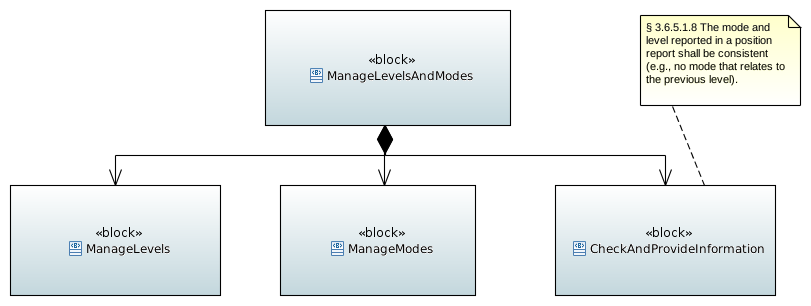
\includegraphics[width=\textwidth]{images/FunctionalArchitecture.png}
\caption{Mode\_and\_Level component SysML diagram}\label{f:mode_and_level_interface}
\end{figure}


\subsubsection{Inputs}\label{s:mode_and_level_inputs}

\paragraph{Data\_From\_TIU}
\todo[inline]{table has been truncated. Please do not remove rows from the table template. Just use "n/a" if a row is not relevant for a paritcular input ot output.}
\begin{longtable}{p{.25\textwidth}p{.7\textwidth}}
\toprule
Input name				& Data\_From\_TIU \\
\midrule
Description				& Set of data providing by TIU \\
\midrule
Source					& input\_from\_TIU\_API\_Pkg::manageTIU\_input \\ 
\midrule
Type					& TIU\_Types\_Pkg::Message\_Train\_Interface\_to\_EVC\_T \\
\midrule
Valid range of values	& It is a complex type
\todo[inline]{more detail should be given here}  \\
\midrule
Behaviour when value is at boundary	& [Description of components behaviour when input value is at boundary]
\todo[inline]{to be completed} \\
\midrule
Behaviour for values out of valid range	& [Description of components behaviour when input value is out of valid range]
\todo[inline]{to be completed} \\
\midrule
Behaviour when value is erroneous, absent or unwanted (i.e. spurious) & [Description of components behaviour when value is erroneous, absent or unwanted (i.e. spurious)]
\todo[inline]{to be completed} \\
\bottomrule
\end{longtable}


\paragraph{Cab\_In}
\todo[inline]{table has been truncated. Please do not remove rows from the table template. Just use "n/a" if a row is not relevant for a paritcular input ot output.}
\begin{longtable}{p{.25\textwidth}p{.7\textwidth}}
\toprule
Input name				& Cab\_In \\
\midrule
Description				& Identification of the cabine where the EVC is implemented \\
\midrule
Source					& ??? 
\todo[inline]{to be completed}\\ 
\midrule
Type					& TIU\_Types\_Pkg::cab\_ID\_T \\
\midrule
Valid range of values	& [CabUndefined, CabA, CabB] \\
\midrule
Behaviour when value is at boundary	& [Description of components behaviour when input value is at boundary]
\todo[inline]{to be completed} \\
\midrule
Behaviour for values out of valid range	& [Description of components behaviour when input value is out of valid range]
\todo[inline]{to be completed} \\
\midrule
Behaviour when value is erroneous, absent or unwanted (i.e. spurious) & [Description of components behaviour when value is erroneous, absent or unwanted (i.e. spurious)]
\todo[inline]{to be completed} \\

\bottomrule
\end{longtable}

\paragraph{Data\_From\_DMI}
\todo[inline]{table has been truncated. Please do not remove rows from the table template. Just use "n/a" if a row is not relevant for a paritcular input ot output.}
\begin{longtable}{p{.25\textwidth}p{.7\textwidth}}
\toprule
Input name				& Data\_From\_DMI \\
\midrule
Description				& Set of data transmitted from DMI  (driver acknowledgements and requests to  switch modes and level) \\
\midrule
Source					& manage\_DMI\_Input\_Pkg::manageDMI\_Input \\ 
\midrule
Type					& DMI\_Types\_Pkg::DMI\_To\_Modes\_T \\
\midrule
Valid range of values	& It is a complex type : \\
& \begin{itemize}
\item valid :  bool,  flag to inform of the freshness of the information
\item DriverAck : DMI\_DriverAck\_T, indicate which mode is acknoledged
\item DriverRequest : DMI\_DriverRequest\_T, table of boolean values for all the driver request related to  mode changes.
\item LevelAck : bool, indication of Level  change acknowledgement
\end{itemize} \\
\midrule
Behaviour when value is at boundary	& [Description of components behaviour when input value is at boundary]
\todo[inline]{to be completed} \\
\midrule
Behaviour for values out of valid range	& [Description of components behaviour when input value is out of valid range]
\todo[inline]{to be completed} \\
\midrule
Behaviour when value is erroneous, absent or unwanted (i.e. spurious) & [Description of components behaviour when value is erroneous, absent or unwanted (i.e. spurious)]
\todo[inline]{to be completed} \\
\bottomrule
\end{longtable}

\paragraph{driver\_level\_transition\_in}
\todo[inline]{table has been truncated. Please do not remove rows from the table template. Just use "n/a" if a row is not relevant for a paritcular input ot output.}
\begin{longtable}{p{.25\textwidth}p{.7\textwidth}}
\toprule
Input name				& driver\_level\_transition\_in \\
\midrule
Description				& Request of level transition given by the driver for example at start of mission \\
\midrule
Source					& manage\_DMI\_Input\_Pkg::manageDMI\_Input \\ 
\midrule
Type					& Level\_And\_Modes\_Types\_Pkg::T\_LevelTransition \\
\midrule
Valid range of values	& It is a complex type \\
\midrule
Behaviour when value is at boundary	& [Description of components behaviour when input value is at boundary]
\todo[inline]{to be completed} \\
\midrule
Behaviour for values out of valid range	& [Description of components behaviour when input value is out of valid range]
\todo[inline]{to be completed} \\
\midrule
Behaviour when value is erroneous, absent or unwanted (i.e. spurious) & [Description of components behaviour when value is erroneous, absent or unwanted (i.e. spurious)]
\todo[inline]{to be completed} \\
\bottomrule
\end{longtable}



\paragraph{Data\_From\_Track\_Packets}
\todo[inline]{table has been truncated. Please do not remove rows from the table template. Just use "n/a" if a row is not relevant for a paritcular input ot output.}
\begin{longtable}{p{.25\textwidth}p{.7\textwidth}}
\toprule
Input name				& Data\_From\_Track\_Packets \\
\midrule
Description				& Packets received from trackside contaigning information for modes and levels switches \\
\midrule
Source					& ???? 
\todo[inline]{to be completed}\\ 
\midrule
Type					& Level\_And\_Mode\_Types\_Pkg::T\_Data\_From\_Track\_Packet \\
\midrule
Valid range of values	& It is a complex type containing the information of packets : 12, 15, 21, 27, 41, 46, 63, 80, 135, 137, 138 and 139 \\
\midrule
Behaviour when value is at boundary	& [Description of components behaviour when input value is at boundary]
\todo[inline]{to be completed} \\
\midrule
Behaviour for values out of valid range	& [Description of components behaviour when input value is out of valid range]
\todo[inline]{to be completed} \\
\midrule
Behaviour when value is erroneous, absent or unwanted (i.e. spurious) & [Description of components behaviour when value is erroneous, absent or unwanted (i.e. spurious)]
\todo[inline]{to be completed} \\
\bottomrule
\end{longtable}


\paragraph{Data\_From\_speed\_and\_Supervision}
\todo[inline]{table has been truncated. Please do not remove rows from the table template. Just use "n/a" if a row is not relevant for a paritcular input ot output.}
\begin{longtable}{p{.25\textwidth}p{.7\textwidth}}
\toprule
Input name				& Data\_From\_speed\_and\_Supervision \\
\midrule
Description				& Data provided by the speed and supervision function \\
\midrule
Source					& Speed and Supervision function
\todo[inline]{Please use exact component name from SCADE model.} \\ 
\midrule
Type					& Level\_And\_Mode\_Types\_Pkg::T\_Data\_From\_Speed\_Supervision \\
\midrule
Valid range of values	& Input type a complex type
\begin{itemize}
\item \emph{Estim\_front\_End\_overpass\_SR\_Dist : bool}: the train overpass the SR distance with its estimated front end (from SR to trip mode condition 42) 
\item \emph{Estim\_Front\_End\_Rear\_SSP : bool}: estimated front end is rear of the start location of either SSP or gradient profile stored on-board (from FS, LS, OS to trip mode condition 69)
\item \emph{Override\_Function\_Active}: boolean to indicate the state of the activation function 	  	
\item \emph{EOA\_Antenna\_Overpass : bool}: the train overpasses the  EOA  with min safe antenna position Level 1 (from FS, LS, OS to trip mode condition 12)
\item \emph{EOA\_Front\_End : bool} the train overpasses the  EOA  with min safe front end, Level 2 or 3 (from FS, LS, OS to trip mode condition 16)
\item \emph{Train\_Speed\_Under\_Overide\_Limit : bool} supervision when override function is active (to SR mode condition 37)
\end{itemize}\\
\midrule
Behaviour when value is at boundary	& [Description of components behaviour when input value is at boundary]
\todo[inline]{to be completed} \\
\midrule
Behaviour for values out of valid range	& [Description of components behaviour when input value is out of valid range]
\todo[inline]{to be completed} \\
\midrule
Behaviour when value is erroneous, absent or unwanted (i.e. spurious) & [Description of components behaviour when value is erroneous, absent or unwanted (i.e. spurious)]
\todo[inline]{to be completed} \\
\bottomrule
\end{longtable}



\subsubsection{Outputs}\label{s:mode_and_level_outputs}
\todo[inline]{Description of outputs needs to be completed}
\paragraph{[Output 1 name]}

\begin{longtable}{p{.25\textwidth}p{.7\textwidth}}
\toprule
Output name				& [Name of the output] \\
\midrule
Description				& [Brief description of the output] \\
\midrule
Destination				& [Name of the destination component(s)] \\ 
\midrule
Type					& [Type of the output] \\
\midrule
Valid range of values	& [Complete list of valid values] \\
\midrule
Behaviour when value is at boundary	& [Description of components behaviour when output value is at boundary] \\
\midrule
Behaviour for values out of valid range	& [Description of components behaviour when output value is out of valid range] \\
\midrule
Behaviour when value is erroneous, absent or unwanted (i.e. spurious) & [Description of components behaviour when value is erroneous, absent or unwanted (i.e. spurious)] \\
\bottomrule
\end{longtable}


\paragraph{[Output 2 name]}

\begin{longtable}{p{.25\textwidth}p{.7\textwidth}}
\toprule
Output name				& [Name of the output] \\
\midrule
Description				& [Brief description of the output] \\
\midrule
Destination				& [Name of the destination component(s)] \\ 
\midrule
Type					& [Type of the output] \\
\midrule
Valid range of values	& [Complete list of valid values] \\
\midrule
Behaviour when value is at boundary	& [Description of components behaviour when output value is at boundary] \\
\midrule
Behaviour for values out of valid range	& [Description of components behaviour when output value is out of valid range] \\
\midrule
Behaviour when value is erroneous, absent or unwanted (i.e. spurious) & [Description of components behaviour when value is erroneous, absent or unwanted (i.e. spurious)] \\
\bottomrule
\end{longtable}


\subsection{Subcomponents}\label{s:mdoe_and_level_subcomponents}

\subsubsection{Level\_Management}
%set the master document for easy compilation
%!TEX root = ../D3_5_3.tex

\paragraph{Component Requirements}

\begin{longtable}{p{.25\textwidth}p{.7\textwidth}}
\toprule
Component name			& Level\_Management \\
\midrule
Link to SCADE model		& {\footnotesize \url{https://github.com/openETCS/modeling/tree/master/openETCS ArchitectureAndDesign/Work Groups/Group 3/SCADE/LevelManagement/}} \\
\midrule
SCADE designer			& Marielle Petit-Doche and  Matthias G\"udemann, Systerel \\
\midrule
Description				& The level management subsystem receives level transition order tables and selects the order with the highest probability. It stores the information about the selected transition order and transits to the requested level once the train passes the location of the level transition.

If required, the driver is asked to acknowledge the transition, in case of no acknowledgment or if conditions for the level transition are not fulfilled, the train gets tripped.

On the most abstract level the design consists of the \emph{manage\_priorities} function which takes the level transition order priority tables as inputs and computes the highest priority transition.

This transition order is the fed to the \emph{computeLevelTransitions} operator. This operator consists of three main parts. The \emph{ComputeTransitionConditions} operator that emits the fulfilled conditions to change from a given level to a new level, the \emph{LevelStateMachine} that stores the current level and takes the computed change conditions as input for possible level transitions and finally the \emph{driverAck} operator which contains a state machine that stores the information whether the system is currently waiting for a driver acknowledge and emits the train trip information if necessary. \\
\midrule
Input documents	& 
Subset-026, Chapter 5.10 \\
\midrule
Safety integrity level		& 4 \\
\midrule
Time constraints		& [If applicable description of time constraints, otherwise n/a] 
\todo[inline]{to be completed}\\
\midrule
API requirements 		& [If applicable description of API requirements, otherwise n/a] 
\todo[inline]{to be completed}\\
\bottomrule
\end{longtable}


\paragraph{Interface}

For an overview of the interface of this internal component we refer to the SCADE model (cf.~link above) respectively the SCADE generated documentation.

\subsubsection{Mode\_Management}
%set the master document for easy compilation
%!TEX root = ../D3_5_2.tex

\paragraph{Component Requirements}

\begin{longtable}{p{.25\textwidth}p{.7\textwidth}}
\toprule
Component name			& Mode\_Management \\
\midrule
Link to SCADE model		& {\footnotesize \url{https://github.com/openETCS/modeling/tree/master/model/Scade/System/ObuFunctions/ManageLevelsAndModes/Modes}} \\
\midrule
SCADE designer			& Marielle Petit-Doche, Systerel \\
\midrule
Description				& This function is in charge of the computation of new mode to apply according to conditions from inputs (track information, driver interactions, train data,...) and other functions.

Three subfunctions are defined:
\begin{description}
\item[Inputs] proceeds to inputs check and preparation.
\item[ComputeModesCondition] performs all specific procedure linked to mode management and defined in  \citep{subset-026} sections 5.4, 5.5, 5.6, 5.7, 5.8, 5.9, 5.11, 5.12, 5.13, 5.19 and specifies the conditions to define a mode transition according condition table of section 4.6.3 of \citep{subset-026}
\item[SwitchModes] performs the mode selection according the conditions and priorities defined in transition table  section 4.6.2 of \citep{subset-026}
\item[Outputs] prepares packet of outputs.
\end{description} \\
\midrule
Input documents	& 
Subset-026, Chapter 4.4, 4.6, 5.4, 5.5, 5.6, 5.7, 5.8, 5.9, 5.11, 5.12, 5.13, 5.19 \\
\midrule
Safety integrity level		& 4 \\
\midrule
Time constraints		& [If applicable description of time constraints, otherwise n/a] \\
\midrule
API requirements 		& [If applicable description of API requirements, otherwise n/a] \\
\bottomrule
\end{longtable}


\paragraph{Interface}

For an overview of the interface of this internal component we refer to the SCADE model (c.f.~link above) respectively the SCADE generated documentation.

\subsubsection{Check\_and\_Provide\_Mode\_and\_Level}
%set the master document for easy compilation
%!TEX root = ../D3_5_3.tex

\paragraph{Component Requirements}

\begin{longtable}{p{.25\textwidth}p{.7\textwidth}}
\toprule
Component name			& Check\_and\_Provide\_Mode\_and\_Level \\
\midrule
Link to SCADE model		& {\footnotesize \url{https://github.com/openETCS/modeling/tree/master/model/Scade/System/ObuFunctions/ManageLevelsAndModes/Modes}} \\
\midrule
SCADE designer			& Marielle Petit-Doche, Systerel \\
\midrule
Description				& Checks compatibility between mode and level and provides outputs. \\
\midrule
Input documents	& 
Subset-026, Chapter 3.6.5 \\
\midrule
Safety integrity level		& 4 \\
\midrule
Time constraints		& [If applicable description of time constraints, otherwise n/a] \\
\midrule
API requirements 		& [If applicable description of API requirements, otherwise n/a] \\
\bottomrule
\end{longtable}


\paragraph{Interface}

For an overview of the interface of this internal component we refer to the SCADE model (c.f.~link above) respectively the SCADE generated documentation.




%set the master document for easy compilation
%!TEX root = ../D3_5_3.tex

\paragraph{Component Requirements}

\begin{longtable}{p{.25\textwidth}p{.7\textwidth}}
\toprule
Component name			& calculateTrainPosition \\
\midrule
Link to SCADE model		& {\footnotesize \url{https://github.com/openETCS/modeling/tree/master/model/Scade/System/ObuFunctions/ManageLocationRelatedInformation/TrainPosition/CalculateTrainPosition}} \\
\midrule
SCADE designer			& Uwe Steinke / Siemens AG \\
\midrule
Description				& The main purpose of the function is to calculate the locations of linked and unlinked balise groups (BGs) and the current train position while the train is running along the track. In detail, the calculateTrainPosition function provides a couple of essential subfunctions for the onboard unit. These are mainly
\begin{itemize}
\item creating and maintaining an obu internal coordinate system for all types of location based data
\item storing all linked and unlinked balise groups resulting from over passing or from announcements (linking information) from the track
\item calculating and maintaining the locations of all stored balise groups during the train trip, based on odometry and linking information
\item permanently calculating the current train position based on odometry and passed balise group information
\item providing the last recently passed linked balise group as the LRBG
\item providing additional position attribute information
\item deleting stored balise groups, when appropriate
\item detecting linking consistency errors
\item determining, if linking is used on board
\end{itemize}
The calculation algorithms for locations and positions are implemented as specified in 
{\footnotesize\url{https://github.com/openETCS/SRS-Analysis/blob/master/System%20Analysis/WorkingRepository/Group4/SUBSET_26_3-6/DetermineTrainLocationProcedures.pdf}} \\
\midrule
Input documents	& 
Subset-026, Chapter 3.6 \\
\midrule
Safety integrity level		& 4 \\
\midrule
Time constraints		& n/a \\
\midrule
API requirements 		& Cf.~interface description of parent component. \\
\bottomrule
\end{longtable}


\paragraph{Interface}

For an overview of the interface of this internal component we refer to the SCADE model (cf.~link above) respectively the SCADE generated documentation.

%An overview of the interface of component calculateTrainPosition is shown in Figure~\ref{f:calculateTrainPosition_interface}. The inputs and outputs are described in detail in Section~\ref{s:calculateTrainPosition_inputs} respectively \ref{s:calculateTrainPosition_outputs}.
%
%\begin{figure}
%\center
%\missingfigure{[Put SysML diagram of component here]}
%\caption{Component SysML diagram}\label{f:calculateTrainPosition_interface}
%\end{figure}
%
%\subsubsection{Inputs}\label{s:calculateTrainPosition_inputs}
%
%\paragraph{currentOdometry}
%
%\begin{longtable}{p{.25\textwidth}p{.7\textwidth}}
%\toprule
%Input name				& currentOdometry \\
%
%\midrule
%Description				& currentOdometry is the actual odometry information as known by the whole EVC model and provided by the models external interface. \newline
%  \\
%\midrule
%Source					& External model interface input \\ 
%\midrule
%Type					& Obu\_BasicTypes\_Pkg::odometry\_T \\  
%\midrule
%Valid range of values	& Obu\_BasicTypes\_Pkg::odometry\_T is a complex data type. \\
%\midrule
%Valid range of values	& Obu\_BasicTypes\_Pkg::odometry\_T is a complex data type. Values are given for each element.\newline Format is: Type Name: range/ list of values
%\begin{itemize}
%\item bool valid: [true | false]. Must be permanently set to "true".
%\item timestamp: (0 - 2147483647). Current time in ms, must be monotonically increasing.
%\item odo: Obu\_BasicTypes\_Pkg::OdometryLocations\_T: current odometry log values with uncertainties; must behave according to {\footnotesize\url{https://github.com/openETCS/SRS-Analysis/blob/master/System%20Analysis/WorkingRepository/Group4/SUBSET_26_3-6/DetermineTrainLocationProcedures.pdf}} [[ 3.1 ]]. Members of OdometryLocations\_T are: 
%\begin{itemize}
%\item o\_nominal: L\_internal\_Type: nominal value in cm.
%\item o\_min:     L\_internal\_Type: \newline min. distance = o\_min2 - o\_min1
%\item o\_max:     L\_internal\_Type: \newline max distance = o\_max2 - o\_max1
%\end{itemize}
%
%\item speed: Obu\_BasicTypes\_Pkg::OdometrySpeeds\_T: not used by calculateTrainPosition
%\item acceleration: Obu\_BasicTypes\_Pkg::A\_internal\_Type: not used by calculateTrainPosition
%\item motionState: \newline [noMotion | Motion]
%\item motionDirection: Obu\_BasicTypes\_Pkg::odoMotionDirection\_T \newline [ unknownDirection | cabAFirst | cabBFirst ]
%\end{itemize}  \\
%
%                     	&  \emph{calculateTrainPosition requires consistent value sets of currentOdometry. calculateTrainPosition itself does not check.}
%\\
%
%\midrule
%Behaviour when value is at boundary	& n/a \\
%\midrule
%Behaviour for values out of valid range	& Enumerated values out of range prohibit code generation. In all other cases, calculateTrainPosition does not have the knowledge for out-of-range checks. \\
%\bottomrule
%\end{longtable}
%
%
%
%\paragraph{msgFromTrack}
%
%\begin{longtable}{p{.25\textwidth}p{.7\textwidth}}
%\toprule
%Input name				& msgFromTrack \\
%
%\midrule
%Description				& With msgFromTrack calculateTrainPosition receives datagrams from balise groups and RBC. \newline
%  \\
%\midrule
%Source					& Manage\_TrackSideInformation\_Integration\_Pkg::Manage\_TrackSideInformation\_Integration/ \\ 
%\midrule
%Type					& Common\_Types\_Pkg::ReceivedMessage\_T \\  
%\midrule
%Valid range of values	& Common\_Types\_Pkg::ReceivedMessage\_T is a complex data type. Values are given for each element.\newline Format is: Type Name: range/ list of values
%\begin{itemize}
%\item bool valid: [true | false]. "true" flags a datagram as received and to be evaluated by calculateTrainPosition. Must be set for exactly 1 clock for each received datagram and stay unset otherwise
%\item source: Common\_Types\_Pkg::MsgSource\_T: Designates the source of the datagram: \newline ( msrc\_undefined | msrc\_Euroradio | msrc\_Eurobalise | msrc\_RadioInfillUnit | msrc\_OBU ) 
%
%\item radioMetaData: Common\_Types\_Pkg::radioMetaData\_T: not used by calculateTrainPosition
%
%\item BG\_Common\_Header: BG\_Types\_Pkg::BG\_Header\_T: Header information received from balise groups, refer to Manage\_TrackSideInformation\_Integration\_Pkg::Manage\_TrackSideInformation\_Integration
%
%\item Radio\_Common\_Header: Radio\_Types\_Pkg::Radio\_TrackTrain\_Header\_T: Header information received from RBC via radio, refer to Manage\_TrackSideInformation\_Integration\_Pkg::Manage\_TrackSideInformation\_Integration
%
%\item packets: Common\_Types\_Types\_Pkg::CompressedPackets\_T: datagram packets, refer to Manage\_TrackSideInformation\_Integration\_Pkg::Manage\_TrackSideInformation\_Integration. calculatesTrainPosition extracts packet 5 (linking information), if available.
%
%\item sendingRBC: Common\_Types\_Types\_Pkg::RBC\_Id\_T: designates the origin RBC and the mobile modem channel used onboard, if received via radio. Refer to Manage\_TrackSideInformation\_Integration\_Pkg::Manage\_TrackSideInformation\_Integration for more detailed information.
%
%\end{itemize}  \\
%
%                     	&  \emph{calculateTrainPosition expects the received information to be consistent and validated before applied to. It does not check, if the information is appropriate due to current EVC mode, level, train or balise orientation. Received balise group or linking information already known by calculateTrainPosition overrides former data.}
%\\
%
%\midrule
%Behaviour when value is at boundary	& n/a \\
%\midrule
%Behaviour for values out of valid range	& Enumerated values out of range prohibit code generation. In all other cases, calculateTrainPosition does not have the knowledge for out-of-range checks. \\
%
%\bottomrule
%\end{longtable}
%
%
%
%
%\paragraph{trainProperties}
%
%\begin{longtable}{p{.25\textwidth}p{.7\textwidth}}
%\toprule
%Input name				& trainProperties \\
%
%\midrule
%Description				& Supplies calculateTrainPosition with train specific properties required for position calculation. \newline
%  \\
%\midrule
%Source					& EVC\_Support\_Pkg::maintainTrainProperties/ \\ 
%\midrule
%Type					& TrainPosition\_Types\_Pck::trainProperties\_T \\  
%\midrule
%Valid range of values	& TrainPosition\_Types\_Pck::trainProperties\_T is a complex data type. Values are given for each element.\newline Format is: Type Name: range/ list of values
%\begin{itemize}
%\item nid\_engine:: NID\_ENGINE as defined by subset 026-7. 
%\item nid\_operational: NID\_OPERATIONAL as defined by subset 026-7. 
%\item l\_train: L\_TRAIN as defined by subset 026-7. 
%
%\item d\_baliseAntenna\_2\_frontend: Obu\_BasicTypes\_Pkg::LocWithInAcc\_T:  Distance from the trains balise antenna to the trains front end, in cm with uncertainties. 
%
%\item d\_frontend\_2\_rearend: Obu\_BasicTypes\_Pkg::LocWithInAcc\_T:  Distance from the trains Distance from the trains front end to rear end, in cm with uncertainties. 
%
%\item locationAccuracy\_DefaultValue: Obu\_BasicTypes\_Pkg::LocWithInAcc\_T:  Default location accuracy of balise groups (subset 026, 3.6.4.3.2), in cm with uncertainties. 
%
%\item centerDetectionAcc\_DefaultValue: Obu\_BasicTypes\_Pkg::LocWithInAcc\_T:  Default  accuracy of balise groups detection of the BTM, in cm with uncertainties. Will be applied, if centerDetectionInaccuracy from BTM is not available, especially for announced and not yet passed BGs. 
%
%\end{itemize}  \\
%
%                     	&  \emph{calculateTrainPosition expects this information to be consistent and validated before applied to.}
%\\
%
%\midrule
%Behaviour when value is at boundary	& n/a \\
%\midrule
%Behaviour for values out of valid range	& Enumerated values out of range prohibit code generation. In all other cases, calculateTrainPosition does not have the knowledge for out-of-range checks. \\
%
%\bottomrule
%\end{longtable}
%
%
%
%\paragraph{passedBG}
%
%\begin{longtable}{p{.25\textwidth}p{.7\textwidth}}
%\toprule
%Input name				& passedBG \\
%
%\midrule
%Description				& Deprecated alternative input to msgFromTrack. Must not be used any more and is subject to be removed in subsequent releases.  \newline
%  \\
%
%\bottomrule
%\end{longtable}
%
%
%\paragraph{reset}
%
%\begin{longtable}{p{.25\textwidth}p{.7\textwidth}}
%\toprule
%Input name				& reset \\
%
%\midrule
%Description				& Resets and keeps calculateTrainPosition at its initial state and deletes all internally stored data. \newline
%  \\
%\midrule
%Source					& To whom it may concern/ \\ 
%\midrule
%Type					& bool \\  
%\midrule
%Valid range of values	& [ false | true ] \\
%
%\midrule
%Behaviour when value is at boundary	& n/a \\
%\midrule
%Behaviour for values out of valid range	& Enumerated values out of range prohibit code generation. \\
%
%\bottomrule
%\end{longtable}
%
%
%\subsubsection{Outputs}\label{s:calculateTrainPosition_outputs}
%
%\paragraph{trainPosition}
%
%\begin{longtable}{p{.25\textwidth}p{.7\textwidth}}
%\toprule
%Output name				& trainPosition \\
%
%\midrule
%Description				& Provides the current train position and LRBG with its attributes. All distance and location computations of the OBU must be based on this information. \newline
%  \\
%\midrule
%Destination				& Any drain component which needs the current train position or  LRBG \\ 
%\midrule
%Type					& TrainPosition\_Types\_Pck::trainPosition\_T \\  
%\midrule
%Valid range of values	& TrainPosition\_Types\_Pck::trainPosition\_T is a complex data type. Values are given for each element.\newline Format is: Type Name: range/ list of values
%\begin{itemize}
%\item valid: bool: [true | false]. Always true, except for exceptional circumstances.
%\item timestamp: Obu\_BasicTypes\_Pkg::T\_internal\_Type: latest time in ms. 
%\item trainPositionIsUnknown: bool: true, if the train position is evaluated as "unknonwn" (refer to subset-026, 3.6.3.1.3.1). 
%\item noCoordinateSystemHasBeenAssigned: bool: refer to subset 026, 3.4.2, 3.6.3.1.4
%\item trainPosition: Obu\_BasicTypes\_Pkg::LocWithInAcc\_T: The calculated train position with uncertainties
%\item estimatedFrontEndPosition: Obu\_BasicTypes\_Pkg::Location\_T: Train front end position in cm.
%\item minSafeFrontEndPosition: Obu\_BasicTypes\_Pkg::Location\_T: Train front end position in cm.
%\item maxSafeFrontEndPostion: Obu\_BasicTypes\_Pkg::Location\_T: Train front end position in cm.
%\item LRBG: TrainPosition\_Types\_Pck::positionedBG\_T: the current LRBG. 
%\item prvLRBG: TrainPosition\_Types\_Pck::positionedBG\_T: the balise group passed previously to LRBG. For type definition, see below.
%\item nominalOrReverseToLRBG: Q\_DLRBG: Orientation of the train in relation to the direction of the LRBG, see subset 026-7.
%\item trainOrientationToLRBG: Q\_DIRLRBG: Orientation of the train in relation to the direction of the LRBG, see subset 026-7.
%\item trainRunningDirectionToLRBG: Q\_DIRTRAIN: Direction of train movement in relation to the LRBG orientation, see subset 026-7.
%\item linkingIsUsedOnboard: bool: Designates, if at least one announced linked BG is ahead
%
%\end{itemize}  \\
%
%                     	&  \emph{calculateTrainPosition provides the train position to whom it concerns and recalculates it with every clock cycle}
%\\
%
%\midrule
%Behaviour when value is at boundary	& n/a \\
%\midrule
%Behaviour for values out of valid range	& n/a \\
%
%\midrule
%Behaviour when value is errorneous, absent or unwanted & n/a \\
%
%\bottomrule
%\end{longtable}
%
%
%\paragraph{BGs}
%
%\begin{longtable}{p{.25\textwidth}p{.7\textwidth}}
%\toprule
%Output name				& BGs \\
%
%\midrule
%Description				& A list of all linked and unlinked balise groups - known to calculateTrainPosition - in the order they are arranged on the track.  \newline
%  \\
%\midrule
%Destination				& Any subsequent component which needs the current collection of balises groups \\ 
%\midrule
%Type					& array of TrainPosition\_Types\_Pck::positionedBG\_T \\  
%\midrule
%Valid range of values	& TrainPosition\_Types\_Pck::positionedBG\_T is a complex data type. Values are given for each array element.\newline Format is: Type Name: range/ list of values
%\begin{itemize}
%\item valid: bool: [true | false]. "true" for every existing balise group.
%\item nid\_c: NID\_C: refer to subset 026-7. 
%\item nid\_bg: NID\_BG: refer to subset 026-7. 
%\item q\_link: Q\_LINK: refer to subset 026-7. 
%\item location: Obu\_BasicTypes\_Pkg::LocWithInAcc\_T: The best known location (with inaccuracies) calculated from linking and from passing information.
%\item seqNoOnTrack: int: Sequence number, specifies the order of the BG passed or expected to be passed
%\item infoFromLinking: TrainPosition\_Types\_Pck::infoFromLinking\_T: Describes a linked BG as announced from the linking BG. Mainly, this information is taken from the linking packet.
%\item infoFromPassing: BG\_Types\_Pkg::passedBG\_T: If the balise group has been passed already, this is the relevant information received from the BG.
%
%\end{itemize}  \\
%
%                     	&  \emph{calculateTrainPosition provides the list of balise groups to whom it concerns.}
%\\
%
%\midrule
%Behaviour when value is at boundary	& n/a \\
%\midrule
%Behaviour for values out of valid range	& n/a \\
%
%\midrule
%Behaviour when value is errorneous, absent or unwanted & n/a \\
%
%\bottomrule
%\end{longtable}
%
%\paragraph{errors}
%
%\begin{longtable}{p{.25\textwidth}p{.7\textwidth}}
%\toprule
%Output name				& errors \\
%
%\midrule
%Description				& Provides a collection of error flags, raised by calculateTrainPosition.  \newline
%  \\
%\midrule
%Destination				& Error handlers and components which need to know of common and linking consistency errors.  \\ 
%\midrule
%Type					& TrainPosition\_Types\_Pck::positionErrors\_T \\  
%\midrule
%Valid range of values	& TrainPosition\_Types\_Pck::positionErrors\_T is a complex data type. Values are given for each array element.\newline Format is: Type Name: range/ list of values
%\begin{itemize}
%\item outOfMemSpace: bool: Memory overrun: a passed or announced BG could not be stored.
%\item passedBG\_foundNotWhereExpected: bool: The currently passed linked BG location does not match its expectation window.
%\item positionCalculation\_inconsistent: A consistency problem arose during position calculation.
%\item linkedBGMissed: bool: The expectation window for an announced BG was passed without detecting the BG.
%\item BGpassedInUnexpectedDirection: bool: The BG was passed in a different orientation than announced via linking.
%\item BG\_LinkingConsistencyError: bool: Linking consistency error (ref. subset 026, 3.16.2.3).
%\item twoConsecutiveLinkedBGs\_missed: bool: 2 consecutive linked balise groups announced by linking are not detected and the end of the expectation window of the second balise group has been passed (subset 026, 3.16.2.7.1).
%\item doubleRepositioningError: bool: Double repositioning error (3.16.2.7.2).
%\item bg: TrainPosition\_Types\_Pck::positionedBG\_T: The corresponding balise group in the case of an error.
%
%\end{itemize}  \\
%
%\midrule
%Behaviour when value is at boundary	& n/a \\
%\midrule
%Behaviour for values out of valid range	& n/a \\
%
%\midrule
%Behaviour when value is errorneous, absent or unwanted & n/a \\
%
%\bottomrule
%\end{longtable}
%


%set the master document for easy compilation
%!TEX root = ../D3_5_2.tex

\section{Train\_Supervision}

\subsection{Component Requirements}

\begin{longtable}{p{.25\textwidth}p{.7\textwidth}}
\toprule
Component name			& TrainSupervision \\
\midrule
Link to SCADE model		& {\footnotesize \url{???}} \\
\midrule
SCADE designer			& Christian Stahl, TWT \\
\midrule
Description				& The task of block ``Train Supervision'' is to monitor the speed of the train and the train location and as such to ensure that the speed remains within the given speed and distance limits. This block is mainly based on \cite[Chapt.~3.13]{subset-026}.

The block ``Train Supervision'' takes as input (1) movement related information such as train speed, train position and acceleration, (2) train related information such as brake information and train length, and (3) track related information such as speed and distance limits and national values.

Based on this information a speed profile is calculated. Speed restrictions create target speeds (targets) that have to be followed. For each such target braking curves are generated to supervise at which location of the track the train must perform the brake. In case of no target restrictions the train may accelerate to the supervised maximum speed of the speed profile. These calculations lead to commands being sent to the driver and the brake system.

The functionality is modeled using eight operators, as shown in Figure~\ref{f:ssv}, which are explained below.

The current status of the analysis of ``Train Supervision'' and a functional breakdown can be found in a separate document, \verb+SpeedSupervision_analysis.pdf+.\\
\midrule
Input documents	& 
Subset-026, Chapter 3.13: Speed and distance monitoring \\
\midrule
Safety integrity level		& 4 \\
\midrule
Time constraints		& [If applicable description of time constraints, otherwise n/a] \\
\midrule
API requirements 		& [If applicable description of API requirements, otherwise n/a] \\
\bottomrule
\end{longtable}


\subsection{Interface}

An overview of the interface of component [component name] is shown in Figure~\ref{f:ssv}. The inputs and outputs are described in detail in Section~\ref{s:template_inputs} respectively \ref{s:template_outputs}.

\begin{figure}
\centering
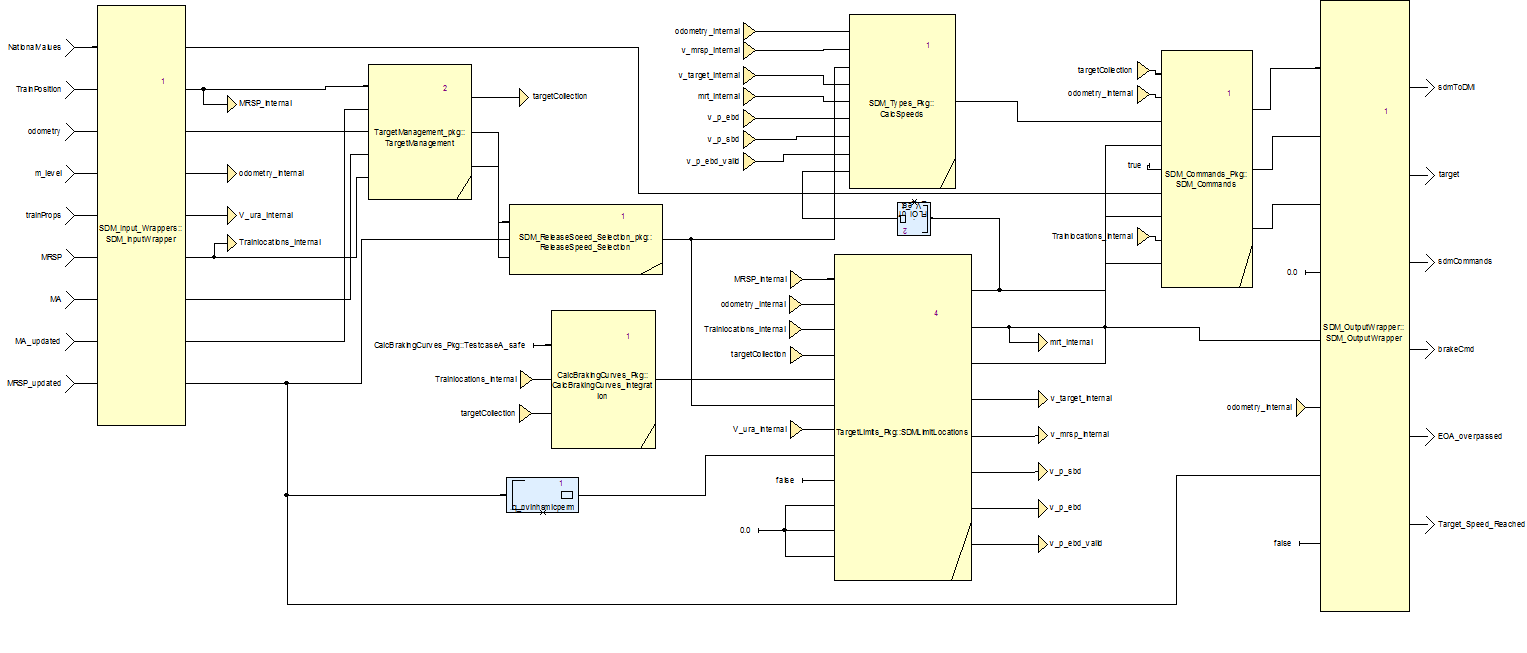
\includegraphics[width=0.95\textheight, angle=90]{../images/speedsupervision.png}
\caption{Structure of component ProvidePositionReport.}\label{f:ssv}
\end{figure}



\subsubsection{Inputs}\label{s:template_inputs}

\paragraph{NationalValues}

\begin{longtable}{p{.25\textwidth}p{.7\textwidth}}
\toprule
Input name				& NationalValues \\
\midrule
Description				& This input is packet 3 of \cite[Chapt.~8]{subset-026}, describing the national values.  \\
\midrule
Source					& ??? \\ 
\midrule
Type					& P3\_NationalValues\_T \\
\midrule
Valid range of values	& [Complete list of valid values] \\
\midrule
Behaviour when value is at boundary	& [Description of components behaviour when input value is at boundary] \\
\midrule
Behaviour for values out of valid range	& [Description of components behaviour when input value is out of valid range] \\
\bottomrule
\end{longtable}


\paragraph{TrainPosition}

\begin{longtable}{p{.25\textwidth}p{.7\textwidth}}
\toprule
Input name				& TrainPosition \\
\midrule
Description				& This input is the current train position. \\
\midrule
Source					& Manage Track Data \\ 
\midrule
Type					& trainPosition\_T \\
\midrule
Valid range of values	& [Complete list of valid values] \\
\midrule
Behaviour when value is at boundary	& [Description of components behaviour when input value is at boundary] \\
\midrule
Behaviour for values out of valid range	& [Description of components behaviour when input value is out of valid range] \\
\bottomrule
\end{longtable}


\paragraph{odometry}

\begin{longtable}{p{.25\textwidth}p{.7\textwidth}}
\toprule
Input name				& odometry \\
\midrule
Description				& This input is the odometry data. \\
\midrule
Source					& Odometry \\ 
\midrule
Type					& odometry\_T \\
\midrule
Valid range of values	& [Complete list of valid values] \\
\midrule
Behaviour when value is at boundary	& [Description of components behaviour when input value is at boundary] \\
\midrule
Behaviour for values out of valid range	& [Description of components behaviour when input value is out of valid range] \\
\bottomrule
\end{longtable}\chapter{[Input 2 name]}


\paragraph{m\_level}

\begin{longtable}{p{.25\textwidth}p{.7\textwidth}}
\toprule
Input name				& m\_level \\
\midrule
Description				& This input is the current level of the train. \\
\midrule
Source					& Mode and Level \\ 
\midrule
Type					& M\_LEVEL \\
\midrule
Valid range of values	& [Complete list of valid values] \\
\midrule
Behaviour when value is at boundary	& [Description of components behaviour when input value is at boundary] \\
\midrule
Behaviour for values out of valid range	& [Description of components behaviour when input value is out of valid range] \\
\bottomrule
\end{longtable}\chapter{[Input 2 name]}

\paragraph{trainProps}

\begin{longtable}{p{.25\textwidth}p{.7\textwidth}}
\toprule
Input name				& trainProps \\
\midrule
Description				& This input is a set of train related properties. \\
\midrule
Source					& Database \\ 
\midrule
Type					& trainProperties\_T \\
\midrule
Valid range of values	& [Complete list of valid values] \\
\midrule
Behaviour when value is at boundary	& [Description of components behaviour when input value is at boundary] \\
\midrule
Behaviour for values out of valid range	& [Description of components behaviour when input value is out of valid range] \\
\bottomrule
\end{longtable}\chapter{[Input 2 name]}


\paragraph{MRSP}

\begin{longtable}{p{.25\textwidth}p{.7\textwidth}}
\toprule
Input name				& MRSP \\
\midrule
Description				& This input is the most restrictive speed profile. \\
\midrule
Source					& ??? \\ 
\midrule
Type					& MRSP\_Profile\_t \\
\midrule
Valid range of values	& [Complete list of valid values] \\
\midrule
Behaviour when value is at boundary	& [Description of components behaviour when input value is at boundary] \\
\midrule
Behaviour for values out of valid range	& [Description of components behaviour when input value is out of valid range] \\
\bottomrule
\end{longtable}\chapter{[Input 2 name]}


\paragraph{MA}

\begin{longtable}{p{.25\textwidth}p{.7\textwidth}}
\toprule
Input name				& MA \\
\midrule
Description				& This input is a movement authority. \\
\midrule
Source					& ??? \\ 
\midrule
Type					& MAs\_t \\
\midrule
Valid range of values	& [Complete list of valid values] \\
\midrule
Behaviour when value is at boundary	& [Description of components behaviour when input value is at boundary] \\
\midrule
Behaviour for values out of valid range	& [Description of components behaviour when input value is out of valid range] \\
\bottomrule
\end{longtable}\chapter{[Input 2 name]}


\paragraph{MA\_updated}

\begin{longtable}{p{.25\textwidth}p{.7\textwidth}}
\toprule
Input name				& MA\_updated \\
\midrule
Description				& This flag is true if the movement authority has been updated in this clock cycle and false otherwise. \\
\midrule
Source					& internal \\ 
\midrule
Type					& bool \\
\midrule
Valid range of values	& [Complete list of valid values] \\
\midrule
Behaviour when value is at boundary	& [Description of components behaviour when input value is at boundary] \\
\midrule
Behaviour for values out of valid range	& [Description of components behaviour when input value is out of valid range] \\
\bottomrule
\end{longtable}


\paragraph{MRSP\_updated}

\begin{longtable}{p{.25\textwidth}p{.7\textwidth}}
\toprule
Input name				& MRSP\_updated \\
\midrule
Description				& This flag is true if the most restrictive speed profile has been updated in this clock cycle and false otherwise. \\
\midrule
Source					& internal \\ 
\midrule
Type					& bool \\
\midrule
Valid range of values	& [Complete list of valid values] \\
\midrule
Behaviour when value is at boundary	& [Description of components behaviour when input value is at boundary] \\
\midrule
Behaviour for values out of valid range	& [Description of components behaviour when input value is out of valid range] \\
\bottomrule
\end{longtable}


\subsubsection{Outputs}\label{s:template_outputs}

\paragraph{[Output 1 name]}

\begin{longtable}{p{.25\textwidth}p{.7\textwidth}}
\toprule
Output name				& [Name of the output] \\
\midrule
Description				& [Brief description of the output] \\
\midrule
Destination				& [Name of the destination component(s)] \\ 
\midrule
Type					& [Type of the output] \\
\midrule
Valid range of values	& [Complete list of valid values] \\
\midrule
Behaviour when value is at boundary	& [Description of components behaviour when output value is at boundary] \\
\midrule
Behaviour for values out of valid range	& [Description of components behaviour when output value is out of valid range] \\
\bottomrule
\end{longtable}


\paragraph{[Output 2 name]}

\begin{longtable}{p{.25\textwidth}p{.7\textwidth}}
\toprule
Output name				& [Name of the output] \\
\midrule
Description				& [Brief description of the output] \\
\midrule
Destination				& [Name of the destination component(s)] \\ 
\midrule
Type					& [Type of the output] \\
\midrule
Valid range of values	& [Complete list of valid values] \\
\midrule
Behaviour when value is at boundary	& [Description of components behaviour when output value is at boundary] \\
\midrule
Behaviour for values out of valid range	& [Description of components behaviour when output value is out of valid range] \\
\bottomrule
\end{longtable}


%set the master document for easy compilation
%!TEX root = ../D3_5_3.tex

\section{F2.8: Provide\_Position\_Report}

\subsection{Component Requirements}

\begin{longtable}{p{.25\textwidth}p{.7\textwidth}}
\toprule
Component name			& Provide\_Position\_Report \\
\midrule
Link to SCADE model		& {\footnotesize \url{https://github.com/openETCS/modeling/blob/master/model/Scade/System/ObuFunctions/ManageLocationRelatedInformation/TrainPosition/ProvidePositionReport/ProvidePositionReport_Pkg.xscade}}\\
\midrule
SCADE designer			& Christian Stahl, TWT GmbH \\
\midrule
Description				& The component builds a position report for the RBC, i.e., message 132, and provides it as an output.  There are two triggers for sending message 132:  
\begin{enumerate}
\item at least one of the triggers of the position report parameters (packet 58) holds or 
\item one of the events enabling the sending of the report occurs.
\end{enumerate} 
As the core position report (i.e., packet 0 or 1) is included in other packets, the
component also provides this core position report at every clock cycle. At most one of the two packets is valid.\\
\midrule
Input documents	& 
Subset-026, Chapter 3.6.5 \\
\midrule
Safety integrity level		& 4 \\
\midrule
Time constraints		& n/a
\\
\midrule
API requirements 		& n/a \\
\bottomrule
\end{longtable}


\subsection{Interface}

An overview of the interface of component Provide\_Position\_Report is shown in Figure~\ref{f:provide_position_report_interface}. The inputs and outputs are described in detail in Section~\ref{s:provide_position_report_inputs} respectively \ref{s:provide_position_report_outputs}. Subcomponents are described in Section~\ref{s:provide_position_report_subcomponents}.

\begin{figure}
\center
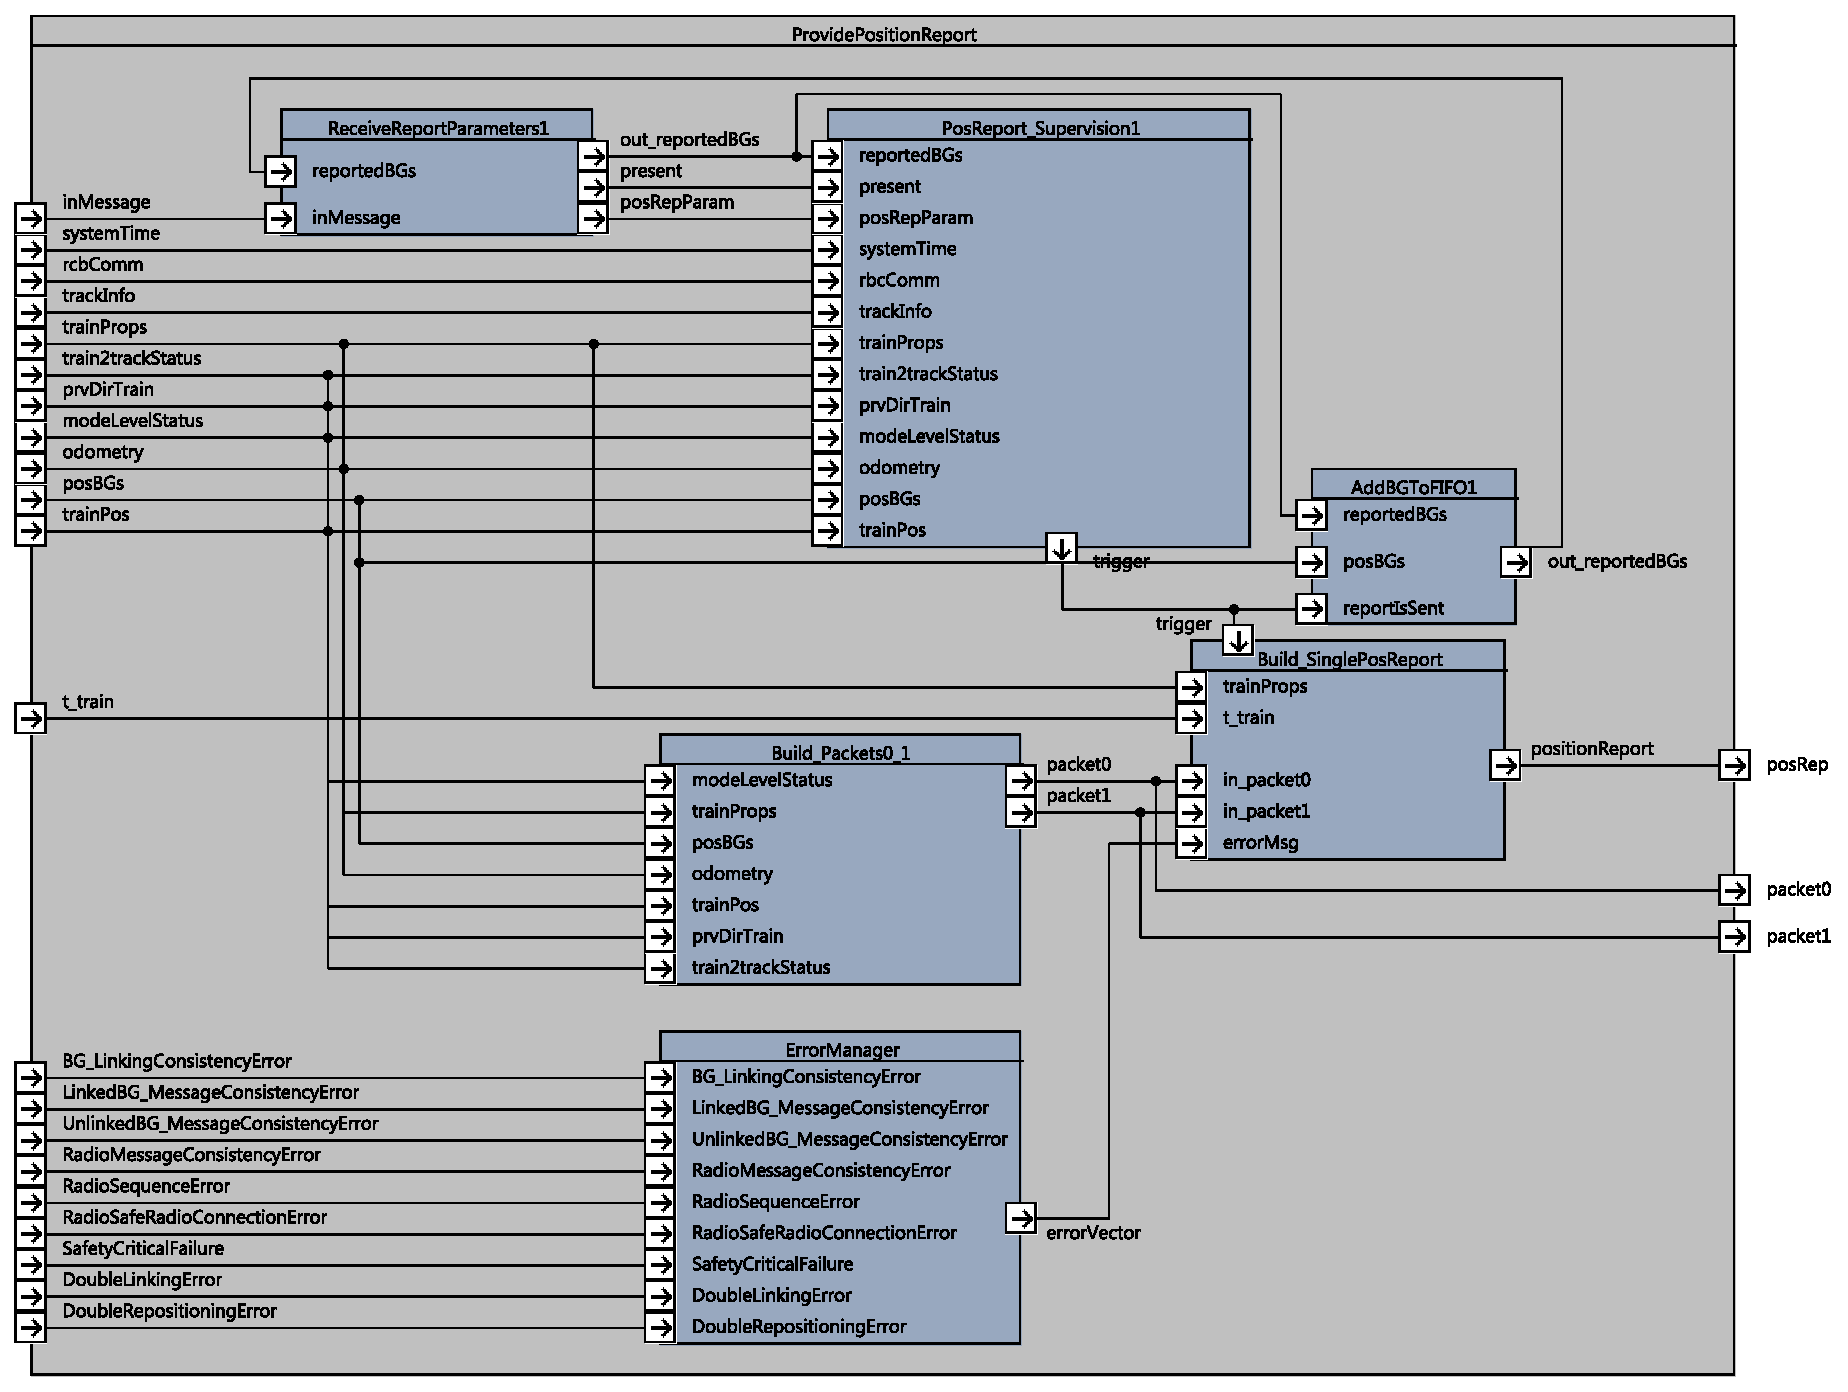
\includegraphics[width=\textwidth]{ProvidePositionReport_SysML}
\caption{Provide\_Position\_Report component SysML diagram}\label{f:provide_position_report_interface}
\end{figure}


\subsubsection{Inputs}\label{s:provide_position_report_inputs}

\paragraph{inMessage}

\begin{longtable}{p{.25\textwidth}p{.7\textwidth}}
\toprule
Input name				& inMessage \\
\midrule
Description				& Input message from the bus (to extract Packet 58, the position report parameters). \\
\midrule
Source					& Manage\_TrackSideInformation\_Integration\_Pkg::\newline Manage\_TrackSideInformation\_Integration \\ 
\midrule
Type					& Common\_Types\_Pkg::ReceivedMessage\_T \\
\midrule
Valid range of values	& as defined in SCADE \\
\midrule
Behaviour when value is at boundary	& n/a \\
\midrule
Behaviour for values out of valid range	& n/a \\
\midrule
Behaviour when value is erroneous, absent or unwanted (i.e. spurious) & If valid is false, then input is ignored. \\
\bottomrule
\end{longtable}


\paragraph{systemTime}

\begin{longtable}{p{.25\textwidth}p{.7\textwidth}}
\toprule
Input name				& systemTime \\
\midrule
Description				& The system time. \\
\midrule
Source					& API \\ 
\midrule
Type					& SystemTime\_T, i.e., Obu\_BasicTypes\_Pkg::T\_internal\_Type \\
\midrule
Valid range of values	& [0; maximum positive int value of target platform] \\
\midrule
Behaviour when value is at boundary	& assumed to be valid \\
\midrule
Behaviour for values out of valid range	& assumed to be valid \\
\midrule
Behaviour when value is erroneous, absent or unwanted (i.e. spurious) & assumed to be valid \\
\bottomrule
\end{longtable}

\paragraph{rbcComm}

\begin{longtable}{p{.25\textwidth}p{.7\textwidth}}
\toprule
Input name				& rbcComm \\
\midrule
Description				& Variables modeling stati regarding the RBC communication. \\
\midrule
Source					& MoRC\_Pck::MoRC\_Main \\ 
\midrule
Type					& RBC\_Communication\_T \\
\midrule
Valid range of values	& as defined in SCADE \\
\midrule
Behaviour when value is at boundary	& n/a \\
\midrule
Behaviour for values out of valid range	& n/a \\
\midrule
Behaviour when value is erroneous, absent or unwanted (i.e. spurious) & n/a \\
\bottomrule
\end{longtable}

\paragraph{trackInfo}

\begin{longtable}{p{.25\textwidth}p{.7\textwidth}}
\toprule
Input name				& trackInfo \\
\midrule
Description				& Location based events. \\
\midrule
Source					& EVC; currently a constant \\ 
\midrule
Type					& LocationBasedEvents\_T \\
\midrule
Valid range of values	& as defined in SCADE \\
\midrule
Behaviour when value is at boundary	& n/a \\
\midrule
Behaviour for values out of valid range	& n/a \\
\midrule
Behaviour when value is erroneous, absent or unwanted (i.e. spurious) & n/a \\
\bottomrule
\end{longtable}

\paragraph{trainProps}

\begin{longtable}{p{.25\textwidth}p{.7\textwidth}}
\toprule
Input name				& trainProps \\
\midrule
Description				& The train properties. \\
\midrule
Source					& EVC\_Support\_Pkg::maintainTrainProperties \\ 
\midrule
Type					& TrainPosition\_Types\_Pck::trainProperties\_T \\
\midrule
Valid range of values	& as defined in SCADE \\
\midrule
Behaviour when value is at boundary	& n/a \\
\midrule
Behaviour for values out of valid range	& n/a \\
\midrule
Behaviour when value is erroneous, absent or unwanted (i.e. spurious) & n/a \\
\bottomrule
\end{longtable}

\paragraph{train2trackStatus}

\begin{longtable}{p{.25\textwidth}p{.7\textwidth}}
\toprule
Input name				& train2trackStatus \\
\midrule
Description				& Train to track status information. \\
\midrule
Source					& EVC \\ 
\midrule
Type					& BG\_Types\_Pkg::TrainToTrackStatus\_T \\
\midrule
Valid range of values	& as defined in SCADE \\
\midrule
Behaviour when value is at boundary	& n/a \\
\midrule
Behaviour for values out of valid range	& n/a \\
\midrule
Behaviour when value is erroneous, absent or unwanted (i.e. spurious) & n/a \\
\bottomrule
\end{longtable}

\paragraph{prvDirTrain}

\begin{longtable}{p{.25\textwidth}p{.7\textwidth}}
\toprule
Input name				& prvDirTrain \\
\midrule
Description				& Train direction of the last clock cycle. \\
\midrule
Source					& CalculateTrainPosition\_Pkg::calculateTrainPosition \\ 
\midrule
Type					& Q\_DIRTRAIN \\
\midrule
Valid range of values	& as defined in SCADE \\
\midrule
Behaviour when value is at boundary	& n/a \\
\midrule
Behaviour for values out of valid range	& n/a \\
\midrule
Behaviour when value is erroneous, absent or unwanted (i.e. spurious) & n/a \\
\bottomrule
\end{longtable}

\paragraph{modeLevelStatus}

\begin{longtable}{p{.25\textwidth}p{.7\textwidth}}
\toprule
Input name				& modeLevelStatus \\
\midrule
Description				& Information referring to mode and level status. \\
\midrule
Source					& ManageLevelAndMode \\ 
\midrule
Type					& ModeLevel2PositionReport\_T \\
\midrule
Valid range of values	& as defined in SCADE \\
\midrule
Behaviour when value is at boundary	& n/a \\
\midrule
Behaviour for values out of valid range	& n/a \\
\midrule
Behaviour when value is erroneous, absent or unwanted (i.e. spurious) & n/a \\
\bottomrule
\end{longtable}

\paragraph{odometry}

\begin{longtable}{p{.25\textwidth}p{.7\textwidth}}
\toprule
Input name				& odometry \\
\midrule
Description				& Odometry information.\\
\midrule
Source					& API \\ 
\midrule
Type					& Obu\_BasicTypes\_Pkg::odometry\_T \\
\midrule
Valid range of values	& as defined in SCADE \\
\midrule
Behaviour when value is at boundary	& n/a \\
\midrule
Behaviour for values out of valid range	& n/a \\
\midrule
Behaviour when value is erroneous, absent or unwanted (i.e. spurious) & n/a \\
\bottomrule
\end{longtable}

\paragraph{posBGs}

\begin{longtable}{p{.25\textwidth}p{.7\textwidth}}
\toprule
Input name				& posBGs \\
\midrule
Description				& Positioned balise groups used for current train position. \\
\midrule
Source					& CalculateTrainPosition\_Pkg::calculateTrainPosition \\ 
\midrule
Type					& TrainPosition\_Types\_Pck::positionedBGs\_T \\
\midrule
Valid range of values	& as defined in SCADE \\
\midrule
Behaviour when value is at boundary	& n/a \\
\midrule
Behaviour for values out of valid range	& n/a \\
\midrule
Behaviour when value is erroneous, absent or unwanted (i.e. spurious) & n/a \\
\bottomrule
\end{longtable}

\paragraph{trainPos}

\begin{longtable}{p{.25\textwidth}p{.7\textwidth}}
\toprule
Input name				& trainPos \\
\midrule
Description				& Current train position. \\
\midrule
Source					& CalculateTrainPosition\_Pkg::calculateTrainPosition \\ 
\midrule
Type					& TrainPosition\_Types\_Pck::trainPosition\_T \\
\midrule
Valid range of values	& as defined in SCADE \\
\midrule
Behaviour when value is at boundary	& n/a \\
\midrule
Behaviour for values out of valid range	& n/a \\
\midrule
Behaviour when value is erroneous, absent or unwanted (i.e. spurious) & n/a \\
\bottomrule
\end{longtable}

\paragraph{t\_train}

\begin{longtable}{p{.25\textwidth}p{.7\textwidth}}
\toprule
Input name				& t\_train \\
\midrule
Description				& Current timestamp. \\
\midrule
Source					& EVC \\ 
\midrule
Type					& T\_TRAIN \\
\midrule
Valid range of values	& as defined in SCADE \\
\midrule
Behaviour when value is at boundary	& n/a \\
\midrule
Behaviour for values out of valid range	& n/a \\
\midrule
Behaviour when value is erroneous, absent or unwanted (i.e. spurious) & n/a \\
\bottomrule
\end{longtable}

\paragraph{BG\_LinkingConsistencyError}

\begin{longtable}{p{.25\textwidth}p{.7\textwidth}}
\toprule
Input name				& BG\_LinkingConsistencyError \\
\midrule
Description				& True if respective error has occurred; otherwise false. \\
\midrule
Source					& CalculateTrainPosition\_Pkg::calculateTrainPosition \\ 
\midrule
Type					& bool \\
\midrule
Valid range of values	& as defined in SCADE \\
\midrule
Behaviour when value is at boundary	& n/a \\
\midrule
Behaviour for values out of valid range	& n/a \\
\midrule
Behaviour when value is erroneous, absent or unwanted (i.e. spurious) & n/a \\
\bottomrule
\end{longtable}

\paragraph{LinkedBG\_MessageConsistencyError}

\begin{longtable}{p{.25\textwidth}p{.7\textwidth}}
\toprule
Input name				& LinkedBG\_MessageConsistencyError \\
\midrule
Description				& True if respective error has occurred; otherwise false. \\
\midrule
Source					& Manage\_TrackSideInformation\_Integration\_Pkg::\newline Manage\_TrackSideInformation\_Integration \\ 
\midrule
Type					& bool \\
\midrule
Valid range of values	& as defined in SCADE \\
\midrule
Behaviour when value is at boundary	& n/a \\
\midrule
Behaviour for values out of valid range	& n/a \\
\midrule
Behaviour when value is erroneous, absent or unwanted (i.e. spurious) & n/a \\
\bottomrule
\end{longtable}

\paragraph{UnlinkedBG\_MessageConsistencyError}

\begin{longtable}{p{.25\textwidth}p{.7\textwidth}}
\toprule
Input name				& UnlinkedBG\_MessageConsistencyError \\
\midrule
Description				& True if respective error has occurred; otherwise false. \\
\midrule
Source					& Manage\_TrackSideInformation\_Integration\_Pkg::\newline Manage\_TrackSideInformation\_Integration \\ 
\midrule
Type					& bool \\
\midrule
Valid range of values	& as defined in SCADE \\
\midrule
Behaviour when value is at boundary	& n/a \\
\midrule
Behaviour for values out of valid range	& n/a \\
\midrule
Behaviour when value is erroneous, absent or unwanted (i.e. spurious) & n/a \\
\bottomrule
\end{longtable}

\paragraph{RadioMessageConsistencyError}

\begin{longtable}{p{.25\textwidth}p{.7\textwidth}}
\toprule
Input name				& RadioMessageConsistencyError \\
\midrule
Description				& True if respective error has occurred; otherwise false. \\
\midrule
Source					& Manage\_TrackSideInformation\_Integration\_Pkg::\newline Manage\_TrackSideInformation\_Integration \\ 
\midrule
Type					& bool \\
\midrule
Valid range of values	& as defined in SCADE \\
\midrule
Behaviour when value is at boundary	& n/a \\
\midrule
Behaviour for values out of valid range	& n/a \\
\midrule
Behaviour when value is erroneous, absent or unwanted (i.e. spurious) & n/a \\
\bottomrule
\end{longtable}

\paragraph{RadioSequenceError}

\begin{longtable}{p{.25\textwidth}p{.7\textwidth}}
\toprule
Input name				& RadioSequenceError \\
\midrule
Description				& True if respective error has occurred; otherwise false. \\
\midrule
Source					& Manage\_TrackSideInformation\_Integration\_Pkg::\newline Manage\_TrackSideInformation\_Integration \\ 
\midrule
Type					& bool \\
\midrule
Valid range of values	& as defined in SCADE \\
\midrule
Behaviour when value is at boundary	& n/a \\
\midrule
Behaviour for values out of valid range	& n/a \\
\midrule
Behaviour when value is erroneous, absent or unwanted (i.e. spurious) & n/a \\
\bottomrule
\end{longtable}

\paragraph{RadioSafeRadioConnectionError}

\begin{longtable}{p{.25\textwidth}p{.7\textwidth}}
\toprule
Input name				& RadioSafeRadioConnectionError \\
\midrule
Description				& True if respective error has occurred; otherwise false. \\
\midrule
Source					& none; currently a constant \\ 
\midrule
Type					& bool \\
\midrule
Valid range of values	& as defined in SCADE \\
\midrule
Behaviour when value is at boundary	& n/a \\
\midrule
Behaviour for values out of valid range	& n/a \\
\midrule
Behaviour when value is erroneous, absent or unwanted (i.e. spurious) & n/a \\
\bottomrule
\end{longtable}

\paragraph{SafetyCriticalFailure}

\begin{longtable}{p{.25\textwidth}p{.7\textwidth}}
\toprule
Input name				& SafetyCriticalFailure \\
\midrule
Description				& True if respective error has occurred; otherwise false. \\
\midrule
Source					& EVC; currently a constant \\ 
\midrule
Type					& bool \\
\midrule
Valid range of values	& as defined in SCADE \\
\midrule
Behaviour when value is at boundary	& n/a \\
\midrule
Behaviour for values out of valid range	& n/a \\
\midrule
Behaviour when value is erroneous, absent or unwanted (i.e. spurious) & n/a \\
\bottomrule
\end{longtable}

\paragraph{DoubleLinkingError}

\begin{longtable}{p{.25\textwidth}p{.7\textwidth}}
\toprule
Input name				& DoubleLinkingError \\
\midrule
Description				& True if respective error has occurred; otherwise false. \\
\midrule
Source					& CalculateTrainPosition\_Pkg::calculateTrainPosition \\ 
\midrule
Type					& bool \\
\midrule
Valid range of values	& as defined in SCADE \\
\midrule
Behaviour when value is at boundary	& n/a \\
\midrule
Behaviour for values out of valid range	& n/a \\
\midrule
Behaviour when value is erroneous, absent or unwanted (i.e. spurious) & n/a \\
\bottomrule
\end{longtable}

\paragraph{DoubleRepositioningError}

\begin{longtable}{p{.25\textwidth}p{.7\textwidth}}
\toprule
Input name				& DoubleRepositioningError \\
\midrule
Description				& True if respective error has occurred; otherwise false. \\
\midrule
Source					& CalculateTrainPosition\_Pkg::calculateTrainPosition \\ 
\midrule
Type					& bool \\
\midrule
Valid range of values	& as defined in SCADE \\
\midrule
Behaviour when value is at boundary	& n/a \\
\midrule
Behaviour for values out of valid range	& n/a \\
\midrule
Behaviour when value is erroneous, absent or unwanted (i.e. spurious) & n/a \\
\bottomrule
\end{longtable}


\subsubsection{Outputs}\label{s:provide_position_report_outputs}

\paragraph{packet0}

\begin{longtable}{p{.25\textwidth}p{.7\textwidth}}
\toprule
Output name				& packet0 \\
\midrule
Description				& Packet 0 -- position report based on a single balise -- is provided every clock cycle. \\
\midrule
Destination				& TrackAtlas::TrackAtlas\\ 
\midrule
Type					& Packet\_TrainTypes\_Pkg::PT0\_PositionReport\_T \\
\midrule
Valid range of values	& as defined in SCADE \\
\midrule
Behaviour when value is at boundary	& n/a \\
\midrule
Behaviour for values out of valid range	& n/a \\
\midrule
Behaviour when value is erroneous, absent or unwanted (i.e. spurious) & n/a \\
\bottomrule
\end{longtable}


\paragraph{packet1}

\begin{longtable}{p{.25\textwidth}p{.7\textwidth}}
\toprule
Output name				& packet1 \\
\midrule
Description				& Packet 1 -- position report based on two balise groups -- is provided every clock cycle. \\
\midrule
Destination				& TrackAtlas::TrackAtlas \\ 
\midrule
Type					& Packet\_TrainTypes\_Pkg::PT1\_PositionReport\_2BG\_T \\
\midrule
Valid range of values	& as defined in SCADE \\
\midrule
Behaviour when value is at boundary	& n/a \\
\midrule
Behaviour for values out of valid range	& n/a \\
\midrule
Behaviour when value is erroneous, absent or unwanted (i.e. spurious) & n/a \\
\bottomrule
\end{longtable}

\paragraph{posRep}

\begin{longtable}{p{.25\textwidth}p{.7\textwidth}}
\toprule
Output name				& posRep \\
\midrule
Description				& Position report to be send to the RBC, i.e. message 136. \\
\midrule
Destination				& radioOutput\_Pkg::collectRadioMessages \\ 
\midrule
Type					& Radio\_Types\_Pkg::Radio\_TrainTrack\_Message\_T \\
\midrule
Valid range of values	& as defined in SCADE \\
\midrule
Behaviour when value is at boundary	& n/a \\
\midrule
Behaviour for values out of valid range	& n/a \\
\midrule
Behaviour when value is erroneous, absent or unwanted (i.e. spurious) & n/a \\
\bottomrule
\end{longtable}


\subsection{Subcomponents}\label{s:provide_position_report_subcomponents}


\subsubsection{ReceiveReportParameters}
%set the master document for easy compilation
%!TEX root = ../D3_5_3.tex

\paragraph{Component Requirements}

\begin{longtable}{p{.25\textwidth}p{.7\textwidth}}
\toprule
Component name			& ReceiveReportParameters \\
\midrule
Link to SCADE model		& {\footnotesize \url{http://???}} \\
\midrule
SCADE designer			& Christian Stahl, TWT \\
\midrule
Description				& The component reads the position report parameters (i.e., packet 58) from the message bus. When a report is received, the BG information provided is used to update the location of respective BG. This BG is being stored in the list of the last 8 BGs. \\
\midrule
Input documents	& 
Subset-026, Chapter ?.?\newline
Subset-026, Chapter ?.?\newline
Subset-026, Chapter ?.?.?\\
\midrule
Safety integrity level		& 4 \\
\midrule
Time constraints		& [If applicable description of time constraints, otherwise n/a] \\
\midrule
API requirements 		& [If applicable description of API requirements, otherwise n/a] \\
\bottomrule
\end{longtable}


\paragraph{Interface}

For an overview of the interface of this internal component we refer to the SCADE model (cf.~link above) respectively the SCADE generated documentation.

\subsubsection{PosReport\_Supervision}
%set the master document for easy compilation
%!TEX root = ../D3_5_3.tex

\paragraph{Component Requirements}

\begin{longtable}{p{.25\textwidth}p{.7\textwidth}}
\toprule
Component name			& PosReport\_Supervision \\
\midrule
Link to SCADE model		& {\footnotesize \url{http://???}} \\
\midrule
SCADE designer			& Christian Stahl, TWT \\
\midrule
Description				& The component supervises trigger (i.e., position report parameter) and events that trigger the sending of a position report. If the output is true, then a report has to be sent. \\
\midrule
Input documents	& 
Subset-026, Chapter ?.?\newline
Subset-026, Chapter ?.?\newline
Subset-026, Chapter ?.?.?\\
\midrule
Safety integrity level		& 4 \\
\midrule
Time constraints		& [If applicable description of time constraints, otherwise n/a] \\
\midrule
API requirements 		& [If applicable description of API requirements, otherwise n/a] \\
\bottomrule
\end{longtable}


\paragraph{Interface}

For an overview of the interface of this internal component we refer to the SCADE model (cf.~link above) respectively the SCADE generated documentation.

\subsubsection{ErrorManager}
%set the master document for easy compilation
%!TEX root = ../D3_5_3.tex

\paragraph{Component Requirements}

\begin{longtable}{p{.25\textwidth}p{.7\textwidth}}
\toprule
Component name			& ErrorManager \\
\midrule
Link to SCADE model		& {\footnotesize \url{http://???}} \\
\midrule
SCADE designer			& Christian Stahl, TWT \\
\midrule
Description				& The component takes all nine possible error messages as an input and aggregates them to a vector. \\
\midrule
Input documents	& 
Subset-026, Chapter ?.?\newline
Subset-026, Chapter ?.?\newline
Subset-026, Chapter ?.?.?\\
\midrule
Safety integrity level		& 4 \\
\midrule
Time constraints		& [If applicable description of time constraints, otherwise n/a] \\
\midrule
API requirements 		& [If applicable description of API requirements, otherwise n/a] \\
\bottomrule
\end{longtable}


\paragraph{Interface}

For an overview of the interface of this internal component we refer to the SCADE model (cf.~link above) respectively the SCADE generated documentation.

\subsubsection{Build\_Packets0\_1}
%set the master document for easy compilation
%!TEX root = ../D3_5_3.tex

\paragraph{Component Requirements}

\begin{longtable}{p{.25\textwidth}p{.7\textwidth}}
\toprule
Component name			& Build\_Packets0\_1 \\
\midrule
Link to SCADE model		& {\footnotesize \url{https://github.com/openETCS/modeling/blob/master/model/Scade/System/ObuFunctions/ManageLocationRelatedInformation/TrainPosition/ProvidePositionReport/ProvidePositionReport_Pkg.xscade}} \\
\midrule
SCADE designer			& Christian Stahl, TWT \\
\midrule
Description				& The component builds packets 0 and 1; at most one of them is valid. \\
\midrule
Input documents	& 
Subset-026, Chapter 3.6.5 \\
\midrule
Safety integrity level		& 4 \\
\midrule
Time constraints		& n/a \\
\midrule
API requirements 		& n/a \\
\bottomrule
\end{longtable}


\paragraph{Interface}

For an overview of the interface of this internal component we refer to the SCADE model (cf.~link above) respectively the SCADE generated documentation.

\subsubsection{Build\_PosReport}
%set the master document for easy compilation
%!TEX root = ../D3_5_3.tex

\paragraph{Component Requirements}

\begin{longtable}{p{.25\textwidth}p{.7\textwidth}}
\toprule
Component name			& Build\_PosReport \\
\midrule
Link to SCADE model		& {\footnotesize \url{https://github.com/openETCS/modeling/blob/master/model/Scade/System/ObuFunctions/ManageLocationRelatedInformation/TrainPosition/ProvidePositionReport/ProvidePositionReport_Pkg.xscade}} \\
\midrule
SCADE designer			& Christian Stahl, TWT \\
\midrule
Description				& This operator builds nine position report messages -- there can be up to nine errors, and for each error an individual report has to be sent.
The fold operator ensures that the first report is invalid if the first error is not present but there exists an error in the error field. In other words,
one valid report will be built. If the errorVector does not contain a single error, 
then at least one report needs to be built (if the operator is triggered). \\
\midrule
Input documents	& 
Subset-026, Chapter 3.6.5 \\
\midrule
Safety integrity level		& 4 \\
\midrule
Time constraints		& n/a
\\
\midrule
API requirements 		& n/a \\
\bottomrule
\end{longtable}


\paragraph{Interface}

For an overview of the interface of this internal component we refer to the SCADE model (cf.~link above) respectively the SCADE generated documentation.

\subsubsection{AddBGToFIFO}
%set the master document for easy compilation
%!TEX root = ../D3_5_3.tex

\paragraph{Component Requirements}

\begin{longtable}{p{.25\textwidth}p{.7\textwidth}}
\toprule
Component name			& AddBGToFIFO \\
\midrule
Link to SCADE model		& {\footnotesize \url{http://???}} \\
\midrule
SCADE designer			& Christian Stahl, TWT \\
\midrule
Description				&  The component adds the current reported BG to the list of BGs for which a report has been sent. Adding of this BG is performed according to the FIFO method. \\
\midrule
Input documents	& 
Subset-026, Chapter ?.?\newline
Subset-026, Chapter ?.?\newline
Subset-026, Chapter ?.?.?\\
\midrule
Safety integrity level		& 4 \\
\midrule
Time constraints		& [If applicable description of time constraints, otherwise n/a] \\
\midrule
API requirements 		& [If applicable description of API requirements, otherwise n/a] \\
\bottomrule
\end{longtable}


\paragraph{Interface}

For an overview of the interface of this internal component we refer to the SCADE model (cf.~link above) respectively the SCADE generated documentation.



%set the master document for easy compilation
%!TEX root = ../D3_5_3.tex

\section{Manage\_Radio\_Communication}

\subsection{Component Requirements}

\begin{longtable}{p{.25\textwidth}p{.7\textwidth}}
\toprule
Component name			& Mode\_and\_Level \\
\midrule
Link to SCADE model		& {\footnotesize \url{???}} \\
\midrule
SCADE designer			& Uwe Steinke, Siemens AG \\
\midrule
Description				& ??? \\
\midrule
Input documents	& 
Subset-026, Chapter 4 \newline
Subset-026, Chapter 5 \\
\midrule
Safety integrity level	& 4 \\
\midrule
Time constraints		& [If applicable description of time constraints, otherwise n/a] \\
\midrule
API requirements 		& [If applicable description of API requirements, otherwise n/a] \\
\bottomrule
\end{longtable}


\subsection{Interface}

An overview of the interface of component Manage\_Radio\_Communication is shown in Figure~\ref{f:manage_radio_communication_interface}. The inputs and outputs are described in detail in Section~\ref{s:manage_radio_communication_inputs} respectively \ref{s:manage_radio_communication_outputs}. Sub components are described in Section~\ref{s:manage_radio_communication_subcomponents}.

\begin{figure}
\center
\missingfigure{[Put SysML diagram of component here]}
\caption{Manage\_Radio\_Communication component SysML diagram}\label{f:manage_radio_communication_interface}
\end{figure}


\subsubsection{Inputs}\label{s:manage_radio_communication_inputs}

\paragraph{[Input 1 name]}

\begin{longtable}{p{.25\textwidth}p{.7\textwidth}}
\toprule
Input name				& [Name of the input] \\
\midrule
Description				& [Brief description of the input] \\
\midrule
Source					& [Name of the source component] \\ 
\midrule
Type					& [Type of the input] \\
\midrule
Valid range of values	& [Complete list of valid values] \\
\midrule
Behaviour when value is at boundary	& [Description of components behaviour when input value is at boundary] \\
\midrule
Behaviour for values out of valid range	& [Description of components behaviour when input value is out of valid range] \\
\midrule
Behaviour when value is erroneous, absent or unwanted (i.e. spurious) & [Description of components behaviour when value is erroneous, absent or unwanted (i.e. spurious)] \\
\bottomrule
\end{longtable}


\paragraph{[Input 2 name]}

\begin{longtable}{p{.25\textwidth}p{.7\textwidth}}
\toprule
Input name				& [Name of the input] \\
\midrule
Description				& [Brief description of the input] \\
\midrule
Source					& [Name of the source component] \\ 
\midrule
Type					& [Type of the input] \\
\midrule
Valid range of values	& [Complete list of valid values] \\
\midrule
Behaviour when value is at boundary	& [Description of components behaviour when input value is at boundary] \\
\midrule
Behaviour for values out of valid range	& [Description of components behaviour when input value is out of valid range] \\
\midrule
Behaviour when value is erroneous, absent or unwanted (i.e. spurious) & [Description of components behaviour when value is erroneous, absent or unwanted (i.e. spurious)] \\
\bottomrule
\end{longtable}


\subsubsection{Outputs}\label{s:manage_radio_communication_outputs}

\paragraph{[Output 1 name]}

\begin{longtable}{p{.25\textwidth}p{.7\textwidth}}
\toprule
Output name				& [Name of the output] \\
\midrule
Description				& [Brief description of the output] \\
\midrule
Destination				& [Name of the destination component(s)] \\ 
\midrule
Type					& [Type of the output] \\
\midrule
Valid range of values	& [Complete list of valid values] \\
\midrule
Behaviour when value is at boundary	& [Description of components behaviour when output value is at boundary] \\
\midrule
Behaviour for values out of valid range	& [Description of components behaviour when output value is out of valid range] \\
\midrule
Behaviour when value is erroneous, absent or unwanted (i.e. spurious) & [Description of components behaviour when value is erroneous, absent or unwanted (i.e. spurious)] \\
\bottomrule
\end{longtable}


\paragraph{[Output 2 name]}

\begin{longtable}{p{.25\textwidth}p{.7\textwidth}}
\toprule
Output name				& [Name of the output] \\
\midrule
Description				& [Brief description of the output] \\
\midrule
Destination				& [Name of the destination component(s)] \\ 
\midrule
Type					& [Type of the output] \\
\midrule
Valid range of values	& [Complete list of valid values] \\
\midrule
Behaviour when value is at boundary	& [Description of components behaviour when output value is at boundary] \\
\midrule
Behaviour for values out of valid range	& [Description of components behaviour when output value is out of valid range] \\
\midrule
Behaviour when value is erroneous, absent or unwanted (i.e. spurious) & [Description of components behaviour when value is erroneous, absent or unwanted (i.e. spurious)] \\
\bottomrule
\end{longtable}


\subsection{Sub Components}\label{s:manage_radio_communication_subcomponents}

\subsubsection{Management\_of\_Radio\_Communication}
%set the master document for easy compilation
%!TEX root = ../D3_5_3.tex

\paragraph{Component Requirements}

\begin{longtable}{p{.25\textwidth}p{.7\textwidth}}
\toprule
Component name			& MoRC\_Main\_v2 (Management\_of\_Radio\_Communication) \\
\midrule
Link to SCADE model		& {\footnotesize \url{https://github.com/openETCS/modeling/tree/master/model/Scade/System/ObuFunctions/Radio/MoRC}} \\
\midrule
SCADE designer			& Uwe Steinke, Siemens \\
\midrule
Description				& 
The function \emph{MoRC\_Main\_v2} implements the session states establishing, maintaining and terminating as described in Subset-026, chap. 3.5. A SCADE state machine reflects this state model  accurately. Within each of the states, the activities needed as long as the state is active, are performed. \newline

\emph{MoRC\_Main\_v2} is related to exactly one of the radio mobile modems onboard, monitors its status and controls the processes of registration to the radio network, connecting to one RBC and establishing a radio session with the RBC. \emph{MoRC\_Main\_v2} communicates with its mobile modem directly via the API.  \newline

As the OBU is required to manage up to two RBCs,  two instances of \emph{MoRC\_Main\_v2} are used.  \newline

In addition, \emph{MoRC\_Main\_v2} generates the radio connection indication for the driver.

\\
\midrule
Input documents	& 
Subset-026, Chapter 3.5 \\
\midrule
Safety integrity level		& 4 \\
\midrule
Time constraints		& Implements several time delays, therefore appropriate clocking required \\
\midrule
API requirements 		& Interfaces to the OBUs mobile modem hardware via API \\
\bottomrule
\end{longtable}


\paragraph{Interface}

For an overview of the interface of this internal component we refer to the SCADE model (cf.~link above) respectively the SCADE generated documentation.




%set the master document for easy compilation
%!TEX root = ../D3_5_3.tex

\section{F2.10: ManageDMIInput}

\subsection{Component Requirements}

\begin{longtable}{p{.25\textwidth}p{.7\textwidth}}
\toprule
Component name			& ManageDMIInput \\
\midrule
Link to SCADE model		& {\footnotesize \url{http://???}} \\
\midrule
SCADE designer			& [Name, affiliation] \\
\midrule
Description				& [Brief description of the components functionality] \\
\midrule
Input documents	& 
Subset-026, Chapter ?.?\newline
Subset-026, Chapter ?.?\newline
Subset-026, Chapter ?.?.?\\
\midrule
Safety integrity level		& 4 \\
\midrule
Time constraints		& [If applicable description of time constraints, otherwise n/a] \\
\midrule
API requirements 		& [If applicable description of API requirements, otherwise n/a] \\
\bottomrule
\end{longtable}


\subsection{Interface}

An overview of the interface of component ManageDMIInput is shown in Figure~\ref{f:ManageDMIInput}. The inputs and outputs are described in detail in Section~\ref{s:ManageDMIInput_inputs} respectively \ref{s:ManageDMIInput_outputs}. Subcomponents are described in Section~\ref{s:ManageDMIInput_subcomponents}.

\begin{figure}
\center
\missingfigure{[Put SysML diagram of component here]}
\caption{ManageDMIInput SysML diagram}\label{f:ManageDMIInput}
\end{figure}


\subsubsection{Inputs}\label{s:ManageDMIInput_inputs}

\paragraph{[Input 1 name]}

\begin{longtable}{p{.25\textwidth}p{.7\textwidth}}
\toprule
Input name				& [Name of the input] \\
\midrule
Description				& [Brief description of the input] \\
\midrule
Source					& [Name of the source component] \\ 
\midrule
Type					& [Type of the input] \\
\midrule
Valid range of values	& [Complete list of valid values] \\
\midrule
Behaviour when value is at boundary	& [Description of components behaviour when input value is at boundary] \\
\midrule
Behaviour for values out of valid range	& [Description of components behaviour when input value is out of valid range] \\
\midrule
Behaviour when value is erroneous, absent or unwanted (i.e. spurious) & [Description of components behaviour when value is erroneous, absent or unwanted (i.e. spurious)] \\
\bottomrule
\end{longtable}


\paragraph{[Input 2 name]}

\begin{longtable}{p{.25\textwidth}p{.7\textwidth}}
\toprule
Input name				& [Name of the input] \\
\midrule
Description				& [Brief description of the input] \\
\midrule
Source					& [Name of the source component] \\ 
\midrule
Type					& [Type of the input] \\
\midrule
Valid range of values	& [Complete list of valid values] \\
\midrule
Behaviour when value is at boundary	& [Description of components behaviour when input value is at boundary] \\
\midrule
Behaviour for values out of valid range	& [Description of components behaviour when input value is out of valid range] \\
\midrule
Behaviour when value is erroneous, absent or unwanted (i.e. spurious) & [Description of components behaviour when value is erroneous, absent or unwanted (i.e. spurious)] \\
\bottomrule
\end{longtable}


\subsubsection{Outputs}\label{s:ManageDMIInput_outputs}

\paragraph{[Output 1 name]}

\begin{longtable}{p{.25\textwidth}p{.7\textwidth}}
\toprule
Output name				& [Name of the output] \\
\midrule
Description				& [Brief description of the output] \\
\midrule
Destination				& [Name of the destination component(s)] \\ 
\midrule
Type					& [Type of the output] \\
\midrule
Valid range of values	& [Complete list of valid values] \\
\midrule
Behaviour when value is at boundary	& [Description of components behaviour when output value is at boundary] \\
\midrule
Behaviour for values out of valid range	& [Description of components behaviour when output value is out of valid range] \\
\midrule
Behaviour when value is erroneous, absent or unwanted (i.e. spurious) & [Description of components behaviour when value is erroneous, absent or unwanted (i.e. spurious)] \\
\bottomrule
\end{longtable}


\paragraph{[Output 2 name]}

\begin{longtable}{p{.25\textwidth}p{.7\textwidth}}
\toprule
Output name				& [Name of the output] \\
\midrule
Description				& [Brief description of the output] \\
\midrule
Destination				& [Name of the destination component(s)] \\ 
\midrule
Type					& [Type of the output] \\
\midrule
Valid range of values	& [Complete list of valid values] \\
\midrule
Behaviour when value is at boundary	& [Description of components behaviour when output value is at boundary] \\
\midrule
Behaviour for values out of valid range	& [Description of components behaviour when output value is out of valid range] \\
\midrule
Behaviour when value is erroneous, absent or unwanted (i.e. spurious) & [Description of components behaviour when value is erroneous, absent or unwanted (i.e. spurious)] \\
\bottomrule
\end{longtable}


\subsection{Subcomponents}\label{s:ManageDMIInput_subcomponents}

Currently ManageDMIInput does not have any subcomponents.

%\subsubsection{ManageTextMessages}
%%set the master document for easy compilation
%!TEX root = ../D3_5_3.tex

\paragraph{Component Requirements}

\begin{longtable}{p{.25\textwidth}p{.7\textwidth}}
\toprule
Component name			& ManageTextMessages \\
\midrule
Link to SCADE model		& {\footnotesize \url{https://github.com/openETCS/modeling/tree/master/model/Scade/System/ObuFunctions/manageData/manageDMI}} \\
\midrule
SCADE designer			& Bernd Hekele, DB Netz AG \\
\midrule
Description				& This subcomponent receives available text messages from within the EVC sources, handles messages according to the priority, and provides an output stack for messages. \\
\midrule
Input documents			& 
ERA ERTMS 015560\newline
ETCS DRIVER MACHINE INTERFACE\newline
ERSA API\\
\midrule
Safety integrity level	& 4 \\
\midrule
Time constraints		&  n/a \\
\midrule
API requirements 		&  n/a \\
\bottomrule
\end{longtable}


\paragraph{Interface}

For an overview of the interface of this internal component we refer to the SCADE model (cf.~link above) respectively the SCADE generated documentation.



%set the master document for easy compilation
%!TEX root = ../D3_5_3.tex

\section{F2.11: ManageDMIOutput}

\todo[inline]{section and subsections need to be completed}

\subsection{Component Requirements}

\begin{longtable}{p{.25\textwidth}p{.7\textwidth}}
\toprule
Component name			& ManageDMIOutput \\
\midrule
Link to SCADE model		& {\footnotesize \url{http://???}} \\
\midrule
SCADE designer			& Bernd Hekele, DB Netz AG \\
\midrule
Description				& [Brief description of the components functionality] \\
\midrule
Input documents	& 
Subset-026, Chapter ?.?\newline
Subset-026, Chapter ?.?\newline
Subset-026, Chapter ?.?.?\\
\midrule
Safety integrity level		& 4 \\
\midrule
Time constraints		& [If applicable description of time constraints, otherwise n/a] \\
\midrule
API requirements 		& [If applicable description of API requirements, otherwise n/a] \\
\bottomrule
\end{longtable}


\subsection{Interface}

An overview of the interface of component ManageDMIOutput is shown in Figure~\ref{f:ManageDMIOutput}. The inputs and outputs are described in detail in Section~\ref{s:ManageDMIOutput_inputs} respectively \ref{s:ManageDMIOutput_outputs}. Subcomponents are described in Section~\ref{s:ManageDMIOutput_subcomponents}.

\begin{figure}
\center
\missingfigure{[Put SysML diagram of component here]}
\caption{ManageDMIOutput SysML diagram}\label{f:ManageDMIOutput}
\end{figure}


\subsubsection{Inputs}\label{s:ManageDMIOutput_inputs}

\paragraph{[Input 1 name]}

\begin{longtable}{p{.25\textwidth}p{.7\textwidth}}
\toprule
Input name				& [Name of the input] \\
\midrule
Description				& [Brief description of the input] \\
\midrule
Source					& [Name of the source component] \\ 
\midrule
Type					& [Type of the input] \\
\midrule
Valid range of values	& [Complete list of valid values] \\
\midrule
Behaviour when value is at boundary	& [Description of components behaviour when input value is at boundary] \\
\midrule
Behaviour for values out of valid range	& [Description of components behaviour when input value is out of valid range] \\
\midrule
Behaviour when value is erroneous, absent or unwanted (i.e. spurious) & [Description of components behaviour when value is erroneous, absent or unwanted (i.e. spurious)] \\
\bottomrule
\end{longtable}


\paragraph{[Input 2 name]}

\begin{longtable}{p{.25\textwidth}p{.7\textwidth}}
\toprule
Input name				& [Name of the input] \\
\midrule
Description				& [Brief description of the input] \\
\midrule
Source					& [Name of the source component] \\ 
\midrule
Type					& [Type of the input] \\
\midrule
Valid range of values	& [Complete list of valid values] \\
\midrule
Behaviour when value is at boundary	& [Description of components behaviour when input value is at boundary] \\
\midrule
Behaviour for values out of valid range	& [Description of components behaviour when input value is out of valid range] \\
\midrule
Behaviour when value is erroneous, absent or unwanted (i.e. spurious) & [Description of components behaviour when value is erroneous, absent or unwanted (i.e. spurious)] \\
\bottomrule
\end{longtable}


\subsubsection{Outputs}\label{s:ManageDMIOutput_outputs}

\paragraph{[Output 1 name]}

\begin{longtable}{p{.25\textwidth}p{.7\textwidth}}
\toprule
Output name				& [Name of the output] \\
\midrule
Description				& [Brief description of the output] \\
\midrule
Destination				& [Name of the destination component(s)] \\ 
\midrule
Type					& [Type of the output] \\
\midrule
Valid range of values	& [Complete list of valid values] \\
\midrule
Behaviour when value is at boundary	& [Description of components behaviour when output value is at boundary] \\
\midrule
Behaviour for values out of valid range	& [Description of components behaviour when output value is out of valid range] \\
\midrule
Behaviour when value is erroneous, absent or unwanted (i.e. spurious) & [Description of components behaviour when value is erroneous, absent or unwanted (i.e. spurious)] \\
\bottomrule
\end{longtable}


\paragraph{[Output 2 name]}

\begin{longtable}{p{.25\textwidth}p{.7\textwidth}}
\toprule
Output name				& [Name of the output] \\
\midrule
Description				& [Brief description of the output] \\
\midrule
Destination				& [Name of the destination component(s)] \\ 
\midrule
Type					& [Type of the output] \\
\midrule
Valid range of values	& [Complete list of valid values] \\
\midrule
Behaviour when value is at boundary	& [Description of components behaviour when output value is at boundary] \\
\midrule
Behaviour for values out of valid range	& [Description of components behaviour when output value is out of valid range] \\
\midrule
Behaviour when value is erroneous, absent or unwanted (i.e. spurious) & [Description of components behaviour when value is erroneous, absent or unwanted (i.e. spurious)] \\
\bottomrule
\end{longtable}

\subsection{Subcomponents}\label{s:ManageDMIOutput_subcomponents}


\subsubsection{cyclicReportToDMI}
%set the master document for easy compilation
%!TEX root = ../D3_5_3.tex

\paragraph{Component Requirements}

\begin{longtable}{p{.25\textwidth}p{.7\textwidth}}
\toprule
Component name			& cyclicReportToDMI \\
\midrule
Link to SCADE model		& {\footnotesize \url{https://github.com/openETCS/modeling/tree/master/model/Scade/System/ObuFunctions/manageData/manageDMI}} \\
\midrule
SCADE designer			& Bernd Hekele, DB Netz AG \\
\midrule
Description				& This subcomponent is responsible for writing and sending Dynamic Packets to the DMI. \\
\midrule
Input documents	& 
ERA ERTMS 015560\newline
ETCS DRIVER MACHINE INTERFACE\newline
ERSA API\\
\midrule
Safety integrity level	& 4 \\
\midrule
Time constraints		& periodically \\
\midrule
API requirements 		& n/a\\
\bottomrule
\end{longtable}


\paragraph{Interface}

For an overview of the interface of this internal component we refer to the SCADE model (cf.~link above) respectively the SCADE generated documentation.

\subsubsection{ManageTextMessages}
%set the master document for easy compilation
%!TEX root = ../D3_5_3.tex

\paragraph{Component Requirements}

\begin{longtable}{p{.25\textwidth}p{.7\textwidth}}
\toprule
Component name			& ManageTextMessages \\
\midrule
Link to SCADE model		& {\footnotesize \url{https://github.com/openETCS/modeling/tree/master/model/Scade/System/ObuFunctions/manageData/manageDMI}} \\
\midrule
SCADE designer			& Bernd Hekele, DB Netz AG \\
\midrule
Description				& This subcomponent receives available text messages from within the EVC sources, handles messages according to the priority, and provides an output stack for messages. \\
\midrule
Input documents			& 
ERA ERTMS 015560\newline
ETCS DRIVER MACHINE INTERFACE\newline
ERSA API\\
\midrule
Safety integrity level	& 4 \\
\midrule
Time constraints		&  n/a \\
\midrule
API requirements 		&  n/a \\
\bottomrule
\end{longtable}


\paragraph{Interface}

For an overview of the interface of this internal component we refer to the SCADE model (cf.~link above) respectively the SCADE generated documentation.

\subsubsection{copyTrackDescription}
%set the master document for easy compilation
%!TEX root = ../D3_5_3.tex

\paragraph{Component Requirements}

\begin{longtable}{p{.25\textwidth}p{.7\textwidth}}
\toprule
Component name			& copyTrackDescription \\
\midrule
Link to SCADE model		& {\footnotesize \url{http://???}} \\
\midrule
SCADE designer			& [Name, affiliation] \\
\midrule
Description				& [Brief description of functionality] \\
\midrule
Input documents	& 
Subset-026, Chapter ?.?\newline
Subset-026, Chapter ?.?\newline
Subset-026, Chapter ?.?.?\\
\midrule
Safety integrity level	& 4 \\
\midrule
Time constraints		& [If applicable description of time constraints, otherwise n/a] \\
\midrule
API requirements 		& [If applicable description of API requirements, otherwise n/a] \\
\bottomrule
\end{longtable}


\paragraph{Interface}

For an overview of the interface of this internal component we refer to the SCADE model (cf.~link above) respectively the SCADE generated documentation.

\subsubsection{toEntryRequest}
%set the master document for easy compilation
%!TEX root = ../D3_5_3.tex

\paragraph{Component Requirements}

\begin{longtable}{p{.25\textwidth}p{.7\textwidth}}
\toprule
Component name			& toEntryRequest \\
\midrule
Link to SCADE model		& {\footnotesize \url{http://???}} \\
\midrule
SCADE designer			& Bernd Hekele, DB Netz AG \\
\midrule
Description				& [Brief description of functionality] \\
\midrule
Input documents	& 
Subset-026, Chapter ?.?\newline
Subset-026, Chapter ?.?\newline
Subset-026, Chapter ?.?.?\\
\midrule
Safety integrity level	& 4 \\
\midrule
Time constraints		& [If applicable description of time constraints, otherwise n/a] \\
\midrule
API requirements 		& [If applicable description of API requirements, otherwise n/a] \\
\bottomrule
\end{longtable}


\paragraph{Interface}

For an overview of the interface of this internal component we refer to the SCADE model (cf.~link above) respectively the SCADE generated documentation.

\subsubsection{sendBrakesToDMI}
%set the master document for easy compilation
%!TEX root = ../D3_5_3.tex

\paragraph{Component Requirements}

\begin{longtable}{p{.25\textwidth}p{.7\textwidth}}
\toprule
Component name			& sendBrakesToDMI \\
\midrule
Link to SCADE model		& {\footnotesize \url{http://???}} \\
\midrule
SCADE designer			& [Name, affiliation] \\
\midrule
Description				& [Brief description of functionality] \\
\midrule
Input documents	& 
Subset-026, Chapter ?.?\newline
Subset-026, Chapter ?.?\newline
Subset-026, Chapter ?.?.?\\
\midrule
Safety integrity level	& 4 \\
\midrule
Time constraints		& [If applicable description of time constraints, otherwise n/a] \\
\midrule
API requirements 		& [If applicable description of API requirements, otherwise n/a] \\
\bottomrule
\end{longtable}


\paragraph{Interface}

For an overview of the interface of this internal component we refer to the SCADE model (cf.~link above) respectively the SCADE generated documentation.

\subsubsection{manageDMI\_Output}
%set the master document for easy compilation
%!TEX root = ../D3_5_3.tex

\paragraph{Component Requirements}

\begin{longtable}{p{.25\textwidth}p{.7\textwidth}}
\toprule
Component name			& manageDMI\_Output \\
\midrule
Link to SCADE model		& {\footnotesize \url{http://???}} \\
\midrule
SCADE designer			& [Name, affiliation] \\
\midrule
Description				& [Brief description of functionality] \\
\midrule
Input documents	& 
Subset-026, Chapter ?.?\newline
Subset-026, Chapter ?.?\newline
Subset-026, Chapter ?.?.?\\
\midrule
Safety integrity level	& 4 \\
\midrule
Time constraints		& [If applicable description of time constraints, otherwise n/a] \\
\midrule
API requirements 		& [If applicable description of API requirements, otherwise n/a] \\
\bottomrule
\end{longtable}


\paragraph{Interface}

For an overview of the interface of this internal component we refer to the SCADE model (cf.~link above) respectively the SCADE generated documentation.

\subsubsection{sendTrainData}
%set the master document for easy compilation
%!TEX root = ../D3_5_3.tex

\paragraph{Component Requirements}

\begin{longtable}{p{.25\textwidth}p{.7\textwidth}}
\toprule
Component name			& sendTrainData \\
\midrule
Link to SCADE model		& {\footnotesize \url{http://???}} \\
\midrule
SCADE designer			& Bernd Hekele, DB Netz AG \\
\midrule
Description				& [Brief description of functionality] \\
\midrule
Input documents	& 
Subset-026, Chapter ?.?\newline
Subset-026, Chapter ?.?\newline
Subset-026, Chapter ?.?.?\\
\midrule
Safety integrity level	& 4 \\
\midrule
Time constraints		& [If applicable description of time constraints, otherwise n/a] \\
\midrule
API requirements 		& [If applicable description of API requirements, otherwise n/a] \\
\bottomrule
\end{longtable}


\paragraph{Interface}

For an overview of the interface of this internal component we refer to the SCADE model (cf.~link above) respectively the SCADE generated documentation.

\subsubsection{sendVersion}
%set the master document for easy compilation
%!TEX root = ../D3_5_3.tex

\paragraph{Component Requirements}

\begin{longtable}{p{.25\textwidth}p{.7\textwidth}}
\toprule
Component name			& sendVersion \\
\midrule
Link to SCADE model		& {\footnotesize \url{http://???}} \\
\midrule
SCADE designer			& Bernd Hekele, DB Netz AG \\
\midrule
Description				& [Brief description of functionality] \\
\midrule
Input documents	& 
Subset-026, Chapter ?.?\newline
Subset-026, Chapter ?.?\newline
Subset-026, Chapter ?.?.?\\
\midrule
Safety integrity level	& 4 \\
\midrule
Time constraints		& [If applicable description of time constraints, otherwise n/a] \\
\midrule
API requirements 		& [If applicable description of API requirements, otherwise n/a] \\
\bottomrule
\end{longtable}


\paragraph{Interface}

For an overview of the interface of this internal component we refer to the SCADE model (cf.~link above) respectively the SCADE generated documentation.

\subsubsection{sendLevelListPkg}
%set the master document for easy compilation
%!TEX root = ../D3_5_3.tex

\paragraph{Component Requirements}

\begin{longtable}{p{.25\textwidth}p{.7\textwidth}}
\toprule
Component name			& sendLevelListPkg \\
\midrule
Link to SCADE model		& {\footnotesize \url{http://???}} \\
\midrule
SCADE designer			& [Name, affiliation] \\
\midrule
Description				& [Brief description of functionality] \\
\midrule
Input documents	& 
Subset-026, Chapter ?.?\newline
Subset-026, Chapter ?.?\newline
Subset-026, Chapter ?.?.?\\
\midrule
Safety integrity level	& 4 \\
\midrule
Time constraints		& [If applicable description of time constraints, otherwise n/a] \\
\midrule
API requirements 		& [If applicable description of API requirements, otherwise n/a] \\
\bottomrule
\end{longtable}


\paragraph{Interface}

For an overview of the interface of this internal component we refer to the SCADE model (cf.~link above) respectively the SCADE generated documentation.









%set the master document for easy compilation
%!TEX root = ../D3_5_3.tex

\section{F2.12: ManageTIUInput}\label{s:F2.12}

\todo[inline]{section and corresponding subsections have to be completed}

\subsection{Component Requirements}

\begin{longtable}{p{.25\textwidth}p{.7\textwidth}}
\toprule
Component name			& ManageTIUInput \\
\midrule
Link to SCADE model		& {\footnotesize \url{http://???}} \\
\midrule
SCADE designer			& Bernd Hekele, DB Netz AG \\
\midrule
Description				& [Brief description of the components functionality] \\
\midrule
Input documents	& 
Subset-026, Chapter ?.?\newline
Subset-026, Chapter ?.?\newline
Subset-026, Chapter ?.?.?\\
\midrule
Safety integrity level		& 4 \\
\midrule
Time constraints		& [If applicable description of time constraints, otherwise n/a] \\
\midrule
API requirements 		& [If applicable description of API requirements, otherwise n/a] \\
\bottomrule
\end{longtable}


\subsection{Interface}

An overview of the interface of component ManageTIUInput is shown in Figure~\ref{f:manageTIUInput}. The inputs and outputs are described in detail in Section~\ref{s:manageTIUInput_inputs} respectively \ref{s:manageTIUInput_outputs}. Subcomponents are described in Section~\ref{s:manageTIUInput_subcomponents}.

\begin{figure}
\center
\missingfigure{[Put SysML diagram of component here]}
\caption{ManageTIUInput SysML diagram}\label{f:manageTIUInput}
\end{figure}


\subsubsection{Inputs}\label{s:manageTIUInput_inputs}

\paragraph{[Input 1 name]}

\begin{longtable}{p{.25\textwidth}p{.7\textwidth}}
\toprule
Input name				& [Name of the input] \\
\midrule
Description				& [Brief description of the input] \\
\midrule
Source					& [Name of the source component] \\ 
\midrule
Type					& [Type of the input] \\
\midrule
Valid range of values	& [Complete list of valid values] \\
\midrule
Behaviour when value is at boundary	& [Description of components behaviour when input value is at boundary] \\
\midrule
Behaviour for values out of valid range	& [Description of components behaviour when input value is out of valid range] \\
\midrule
Behaviour when value is erroneous, absent or unwanted (i.e. spurious) & [Description of components behaviour when value is erroneous, absent or unwanted (i.e. spurious)] \\
\bottomrule
\end{longtable}


\paragraph{[Input 2 name]}

\begin{longtable}{p{.25\textwidth}p{.7\textwidth}}
\toprule
Input name				& [Name of the input] \\
\midrule
Description				& [Brief description of the input] \\
\midrule
Source					& [Name of the source component] \\ 
\midrule
Type					& [Type of the input] \\
\midrule
Valid range of values	& [Complete list of valid values] \\
\midrule
Behaviour when value is at boundary	& [Description of components behaviour when input value is at boundary] \\
\midrule
Behaviour for values out of valid range	& [Description of components behaviour when input value is out of valid range] \\
\midrule
Behaviour when value is erroneous, absent or unwanted (i.e. spurious) & [Description of components behaviour when value is erroneous, absent or unwanted (i.e. spurious)] \\
\bottomrule
\end{longtable}


\subsubsection{Outputs}\label{s:manageTIUInput_outputs}

\paragraph{[Output 1 name]}

\begin{longtable}{p{.25\textwidth}p{.7\textwidth}}
\toprule
Output name				& [Name of the output] \\
\midrule
Description				& [Brief description of the output] \\
\midrule
Destination				& [Name of the destination component(s)] \\ 
\midrule
Type					& [Type of the output] \\
\midrule
Valid range of values	& [Complete list of valid values] \\
\midrule
Behaviour when value is at boundary	& [Description of components behaviour when output value is at boundary] \\
\midrule
Behaviour for values out of valid range	& [Description of components behaviour when output value is out of valid range] \\
\midrule
Behaviour when value is erroneous, absent or unwanted (i.e. spurious) & [Description of components behaviour when value is erroneous, absent or unwanted (i.e. spurious)] \\
\bottomrule
\end{longtable}


\paragraph{[Output 2 name]}

\begin{longtable}{p{.25\textwidth}p{.7\textwidth}}
\toprule
Output name				& [Name of the output] \\
\midrule
Description				& [Brief description of the output] \\
\midrule
Destination				& [Name of the destination component(s)] \\ 
\midrule
Type					& [Type of the output] \\
\midrule
Valid range of values	& [Complete list of valid values] \\
\midrule
Behaviour when value is at boundary	& [Description of components behaviour when output value is at boundary] \\
\midrule
Behaviour for values out of valid range	& [Description of components behaviour when output value is out of valid range] \\
\midrule
Behaviour when value is erroneous, absent or unwanted (i.e. spurious) & [Description of components behaviour when value is erroneous, absent or unwanted (i.e. spurious)] \\
\bottomrule
\end{longtable}

\subsection{Subcomponents}\label{s:manageTIUInput_subcomponents}

\subsubsection{mergeTIU\_Info}
%set the master document for easy compilation
%!TEX root = ../D3_5_3.tex

\paragraph{Component Requirements}

\begin{longtable}{p{.25\textwidth}p{.7\textwidth}}
\toprule
Component name			& mergeTIU\_Info \\
\midrule
Link to SCADE model		& {\footnotesize \url{https://github.com/openETCS/modeling/tree/master/model/Scade/System/ObuFunctions/manageData/manageTIU}} \\
\midrule
SCADE designer			& Bernd Hekele, DB Netz AG \\
\midrule
Description				&  This interface is included to cut the traction power. This is used when the ETCS onboard equipment is applying either the service or emergency brakes and needs to ensure that tractive effort is no longer being applied \\
\midrule
Input documents	& 
Alstom API\newline
Subset-034\\
\midrule
Safety integrity level	& 4 \\
\midrule
Time constraints		&\todo[inline]{section and corresponding subsections have to be completed} \\
\midrule
API requirements 		&\todo[inline]{section and corresponding subsections have to be completed} \\
\bottomrule
\end{longtable}


\paragraph{Interface}

For an overview of the interface of this internal component we refer to the SCADE model (cf.~link above) respectively the SCADE generated documentation.

\subsubsection{getTIUStatusFromData}
%set the master document for easy compilation
%!TEX root = ../D3_5_3.tex

\paragraph{Component Requirements}

\begin{longtable}{p{.25\textwidth}p{.7\textwidth}}
\toprule
Component name			& getTIUStatusFromData \\
\midrule
Link to SCADE model		& {\footnotesize \url{https://github.com/openETCS/modeling/tree/master/model/Scade/System/ObuFunctions/manageData/manageTIU}} \\
\midrule
SCADE designer			& Bernd Hekele, DB Netz AG \\
\midrule
Description				& [Brief description of functionality] \\
\midrule
Input documents	& 
Alstom API\newline
Subset-034\\
\midrule
Safety integrity level	& 4 \\
\midrule
Time constraints		&\todo[inline]{section and corresponding subsections have to be completed} \\
\midrule
API requirements 		&\todo[inline]{section and corresponding subsections have to be completed} \\
\bottomrule
\end{longtable}


\paragraph{Interface}

For an overview of the interface of this internal component we refer to the SCADE model (cf.~link above) respectively the SCADE generated documentation.

%set the master document for easy compilation
%!TEX root = ../D3_5_3.tex

\section{F2.13: ManageTIUOutput}

\subsection{Component Requirements}

\begin{longtable}{p{.25\textwidth}p{.7\textwidth}}
\toprule
Component name			& ManageTIUOutput \\
\midrule
Link to SCADE model		& {\footnotesize \url{http://???}} \\
\midrule
SCADE designer			& Bernd Hekele, DB Netz AG \\
\midrule
Description				& [Brief description of the components functionality] \\
\midrule
Input documents	& 
Subset-026, Chapter ?.?\newline
Subset-026, Chapter ?.?\newline
Subset-026, Chapter ?.?.?\\
\midrule
Safety integrity level		& 4 \\
\midrule
Time constraints		& [If applicable description of time constraints, otherwise n/a] \\
\midrule
API requirements 		& [If applicable description of API requirements, otherwise n/a] \\
\bottomrule
\end{longtable}


\subsection{Interface}

An overview of the interface of component ManageTIUOutput is shown in Figure~\ref{f:manageTIUOutput}. The inputs and outputs are described in detail in Section~\ref{s:manageTIUOutput_inputs} respectively \ref{s:manageTIUOutput_outputs}. Subcomponents are described in Section~\ref{s:manageTIUOutput_subcomponents}.

\begin{figure}
\center
\missingfigure{[Put SysML diagram of component here]}
\caption{ManageTIUOutput SysML diagram}\label{f:manageTIUOutput}
\end{figure}


\subsubsection{Inputs}\label{s:manageTIUOutput_inputs}

\paragraph{[Input 1 name]}

\begin{longtable}{p{.25\textwidth}p{.7\textwidth}}
\toprule
Input name				& [Name of the input] \\
\midrule
Description				& [Brief description of the input] \\
\midrule
Source					& [Name of the source component] \\ 
\midrule
Type					& [Type of the input] \\
\midrule
Valid range of values	& [Complete list of valid values] \\
\midrule
Behaviour when value is at boundary	& [Description of components behaviour when input value is at boundary] \\
\midrule
Behaviour for values out of valid range	& [Description of components behaviour when input value is out of valid range] \\
\midrule
Behaviour when value is erroneous, absent or unwanted (i.e. spurious) & [Description of components behaviour when value is erroneous, absent or unwanted (i.e. spurious)] \\
\bottomrule
\end{longtable}


\paragraph{[Input 2 name]}

\begin{longtable}{p{.25\textwidth}p{.7\textwidth}}
\toprule
Input name				& [Name of the input] \\
\midrule
Description				& [Brief description of the input] \\
\midrule
Source					& [Name of the source component] \\ 
\midrule
Type					& [Type of the input] \\
\midrule
Valid range of values	& [Complete list of valid values] \\
\midrule
Behaviour when value is at boundary	& [Description of components behaviour when input value is at boundary] \\
\midrule
Behaviour for values out of valid range	& [Description of components behaviour when input value is out of valid range] \\
\midrule
Behaviour when value is erroneous, absent or unwanted (i.e. spurious) & [Description of components behaviour when value is erroneous, absent or unwanted (i.e. spurious)] \\
\bottomrule
\end{longtable}


\subsubsection{Outputs}\label{s:manageTIUOutput_outputs}

\paragraph{[Output 1 name]}

\begin{longtable}{p{.25\textwidth}p{.7\textwidth}}
\toprule
Output name				& [Name of the output] \\
\midrule
Description				& [Brief description of the output] \\
\midrule
Destination				& [Name of the destination component(s)] \\ 
\midrule
Type					& [Type of the output] \\
\midrule
Valid range of values	& [Complete list of valid values] \\
\midrule
Behaviour when value is at boundary	& [Description of components behaviour when output value is at boundary] \\
\midrule
Behaviour for values out of valid range	& [Description of components behaviour when output value is out of valid range] \\
\midrule
Behaviour when value is erroneous, absent or unwanted (i.e. spurious) & [Description of components behaviour when value is erroneous, absent or unwanted (i.e. spurious)] \\
\bottomrule
\end{longtable}


\paragraph{[Output 2 name]}

\begin{longtable}{p{.25\textwidth}p{.7\textwidth}}
\toprule
Output name				& [Name of the output] \\
\midrule
Description				& [Brief description of the output] \\
\midrule
Destination				& [Name of the destination component(s)] \\ 
\midrule
Type					& [Type of the output] \\
\midrule
Valid range of values	& [Complete list of valid values] \\
\midrule
Behaviour when value is at boundary	& [Description of components behaviour when output value is at boundary] \\
\midrule
Behaviour for values out of valid range	& [Description of components behaviour when output value is out of valid range] \\
\midrule
Behaviour when value is erroneous, absent or unwanted (i.e. spurious) & [Description of components behaviour when value is erroneous, absent or unwanted (i.e. spurious)] \\
\bottomrule
\end{longtable}

\subsection{Subcomponents}\label{s:manageTIUOutput_subcomponents}

\subsubsection{handleTraction}
%set the master document for easy compilation
%!TEX root = ../D3_5_3.tex

\paragraph{Component Requirements}

\begin{longtable}{p{.25\textwidth}p{.7\textwidth}}
\toprule
Component name			& handleTraction \\
\midrule
Link to SCADE model		& {\footnotesize \url{http://???}} \\
\midrule
SCADE designer			& Bernd Hekele, DB Netz AG \\
\midrule
Description				& [Brief description of functionality] \\
\midrule
Input documents	& 
Subset-026, Chapter ?.?\newline
Subset-026, Chapter ?.?\newline
Subset-026, Chapter ?.?.?\\
\midrule
Safety integrity level	& 4 \\
\midrule
Time constraints		& [If applicable description of time constraints, otherwise n/a] \\
\midrule
API requirements 		& [If applicable description of API requirements, otherwise n/a] \\
\bottomrule
\end{longtable}


\paragraph{Interface}

For an overview of the interface of this internal component we refer to the SCADE model (cf.~link above) respectively the SCADE generated documentation.

\subsubsection{manageTIU\_output}
%set the master document for easy compilation
%!TEX root = ../D3_5_3.tex

\paragraph{Component Requirements}

\begin{longtable}{p{.25\textwidth}p{.7\textwidth}}
\toprule
Component name			& manageTIU\_output \\
\midrule
Link to SCADE model		& {\footnotesize \url{http://???}} \\
\midrule
SCADE designer			& Bernd Hekele, DB Netz AG \\
\midrule
Description				& [Brief description of functionality] \\
\midrule
Input documents	& 
Subset-026, Chapter ?.?\newline
Subset-026, Chapter ?.?\newline
Subset-026, Chapter ?.?.?\\
\midrule
Safety integrity level	& 4 \\
\midrule
Time constraints		& [If applicable description of time constraints, otherwise n/a] \\
\midrule
API requirements 		& [If applicable description of API requirements, otherwise n/a] \\
\bottomrule
\end{longtable}


\paragraph{Interface}

For an overview of the interface of this internal component we refer to the SCADE model (cf.~link above) respectively the SCADE generated documentation.


\chapter{F3: Measure Train Movement}
This component is not part of the openETCS OBU currently and therefore no detailed description is provided here.

\chapter{F4: Manage Radio Communication}
This component is not part of the openETCS OBU currently and therefore no detailed description is provided here.

\chapter{F5: Manage JRU}
This component is not part of the openETCS OBU currently and therefore no detailed description is provided here.

\chapter{F6: DMI Controller}
%set the master document for easy compilation
%!TEX root = ../D3_5_2.tex

\section{DMI}

\subsection{Component Requirements}

\begin{longtable}{p{.25\textwidth}p{.7\textwidth}}
\toprule
Component name			& DMI \\
\midrule
Link to SCADE model		& {\footnotesize \url{https://github.com/openETCS/modeling/tree/master/model/Scade/System/DMI_Control}} \\
\midrule
SCADE designer			& Valerio D'Angelo, DB Netz AG \\
\midrule
Description				& The DMI controller interact with the DMI display and is responsible for alls procedures between the DMI display and Driver. Furthermore, the DMI controller will interact with the DMI Management to compute the received information (e.g. driver number request, ...) and send, if necessary, data or reports to the DMI Management (acknowledge, text messages...). The DMI Controller is a passive module, this means that all the processing are performed EVC-side, therefore the DMI Controller simply responds to the requests of the EVC or Driver and performs some checks according with the information received from EVC. \\
\midrule
Input documents	& 
ERA\_ERTMS\_015560 \\
\midrule
Safety integrity level	& 4 \\
\midrule
Time constraints		& [If applicable description of time constraints, otherwise n/a] \\
\midrule
API requirements 		& [If applicable description of API requirements, otherwise n/a] \\
\bottomrule
\end{longtable}


\subsection{Interface}

An overview of the interface of component Mode\_and\_Level is shown in Figure~\ref{f:DMI_interface}. The inputs and outputs are described in detail in Section~\ref{s:DMI_inputs} respectively \ref{s:DMI_outputs}.

\begin{figure}
\center
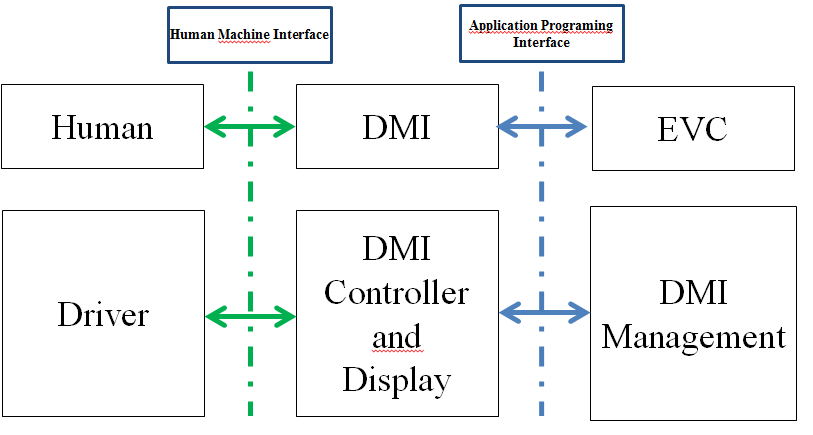
\includegraphics[width=.8\textwidth]{images/DMI_Interfaces}
\caption{Component SysML diagram}\label{f:DMI_interface}
\end{figure}


\subsubsection{Inputs}\label{s:DMI_inputs}

\paragraph{[Input 1 name]}

\begin{longtable}{p{.25\textwidth}p{.7\textwidth}}
\toprule
Input name				& [Name of the input] \\
\midrule
Description				& [Brief description of the input] \\
\midrule
Source					& [Name of the source component] \\ 
\midrule
Type					& [Type of the input] \\
\midrule
Valid range of values	& [Complete list of valid values] \\
\midrule
Behaviour when value is at boundary	& [Description of components behaviour when input value is at boundary] \\
\midrule
Behaviour for values out of valid range	& [Description of components behaviour when input value is out of valid range] \\
\bottomrule
\end{longtable}


\paragraph{[Input 2 name]}

\begin{longtable}{p{.25\textwidth}p{.7\textwidth}}
\toprule
Input name				& [Name of the input] \\
\midrule
Description				& [Brief description of the input] \\
\midrule
Source					& [Name of the source component] \\ 
\midrule
Type					& [Type of the input] \\
\midrule
Valid range of values	& [Complete list of valid values] \\
\midrule
Behaviour when value is at boundary	& [Description of components behaviour when input value is at boundary] \\
\midrule
Behaviour for values out of valid range	& [Description of components behaviour when input value is out of valid range] \\
\bottomrule
\end{longtable}


\subsubsection{Outputs}\label{s:DMI_outputs}

\paragraph{[Output 1 name]}

\begin{longtable}{p{.25\textwidth}p{.7\textwidth}}
\toprule
Output name				& [Name of the output] \\
\midrule
Description				& [Brief description of the output] \\
\midrule
Destination				& [Name of the destination component(s)] \\ 
\midrule
Type					& [Type of the output] \\
\midrule
Valid range of values	& [Complete list of valid values] \\
\midrule
Behaviour when value is at boundary	& [Description of components behaviour when output value is at boundary] \\
\midrule
Behaviour for values out of valid range	& [Description of components behaviour when output value is out of valid range] \\
\bottomrule
\end{longtable}


\paragraph{[Output 2 name]}

\begin{longtable}{p{.25\textwidth}p{.7\textwidth}}
\toprule
Output name				& [Name of the output] \\
\midrule
Description				& [Brief description of the output] \\
\midrule
Destination				& [Name of the destination component(s)] \\ 
\midrule
Type					& [Type of the output] \\
\midrule
Valid range of values	& [Complete list of valid values] \\
\midrule
Behaviour when value is at boundary	& [Description of components behaviour when output value is at boundary] \\
\midrule
Behaviour for values out of valid range	& [Description of components behaviour when output value is out of valid range] \\
\bottomrule
\end{longtable}


\subsection{Sub Components}

%\subsubsection{Management\_of\_Radio\_Communication}
%%set the master document for easy compilation
%!TEX root = ../D3_5_3.tex

\paragraph{Component Requirements}

\begin{longtable}{p{.25\textwidth}p{.7\textwidth}}
\toprule
Component name			& MoRC\_Main\_v2 (Management\_of\_Radio\_Communication) \\
\midrule
Link to SCADE model		& {\footnotesize \url{https://github.com/openETCS/modeling/tree/master/model/Scade/System/ObuFunctions/Radio/MoRC}} \\
\midrule
SCADE designer			& Uwe Steinke, Siemens \\
\midrule
Description				& 
The function \emph{MoRC\_Main\_v2} implements the session states establishing, maintaining and terminating as described in Subset-026, chap. 3.5. A SCADE state machine reflects this state model  accurately. Within each of the states, the activities needed as long as the state is active, are performed. \newline

\emph{MoRC\_Main\_v2} is related to exactly one of the radio mobile modems onboard, monitors its status and controls the processes of registration to the radio network, connecting to one RBC and establishing a radio session with the RBC. \emph{MoRC\_Main\_v2} communicates with its mobile modem directly via the API.  \newline

As the OBU is required to manage up to two RBCs,  two instances of \emph{MoRC\_Main\_v2} are used.  \newline

In addition, \emph{MoRC\_Main\_v2} generates the radio connection indication for the driver.

\\
\midrule
Input documents	& 
Subset-026, Chapter 3.5 \\
\midrule
Safety integrity level		& 4 \\
\midrule
Time constraints		& Implements several time delays, therefore appropriate clocking required \\
\midrule
API requirements 		& Interfaces to the OBUs mobile modem hardware via API \\
\bottomrule
\end{longtable}


\paragraph{Interface}

For an overview of the interface of this internal component we refer to the SCADE model (cf.~link above) respectively the SCADE generated documentation.





\bibliographystyle{unsrt}
\bibliography{architecture}


%\addcontentsline{toc}{chapter}{Index}
%\printindex
%===================================================
%Do NOT change anything below this line

\end{document}
